\documentclass[12pt]{exam}

\newcommand{\Version}{6} 
\newcommand{\Solutions}{0} 
\newcommand{\TestName}{}
\newcommand{\ID}{}


% LOAD PACKAGES
\usepackage{amsmath} % allows for align env and other things
\usepackage{amssymb} % 
\usepackage{mathtools} % allows for single apostrophe
\usepackage{enumitem} % allows for alpha lettering in enumerated lists
\usepackage{lastpage}
\usepackage{array} % for table alignments

\usepackage{graphicx} % if images are needed
\usepackage{wrapfig} % to allow text wrapping

\addpoints

\usepackage{pgfplots} % for surfaces (chapter 7)
\usepackage{tikz-3dplot} 
\pgfplotsset{compat=1.9}
\usetikzlibrary{decorations.pathmorphing,patterns} % for some tikz diagrams
% ~~~~~~~~~~~~~~~~~~~~~~~~~~~~~~~~~~~~
% INITIALS
\newcommand{\Initials}{\textit{\Course, \TestName. Your initials: \underline{\hspace{3cm}}} \vspace{1pt}}

\newcommand{\InitialsLeft}{\noindent \hspace{-18pt}\textit{\Course, \TestName. Your initials: \underline{\hspace{3cm}}} \vspace{1pt}}

\newcommand{\InitialsRight}{\begin{flushright}\textit{\Course, \TestName. Your initials: \underline{\hspace{3cm}}} \vspace{1pt}\end{flushright}}

% ADJUST FIRST LINE IN PARAGRAPH INDENTATION 
\setlength\parindent{0pt}

% FONT FORMAT
\renewcommand*\rmdefault{lmss} % change font to lat mod ss

% ADJUST MARGINS 
\usepackage[a4paper, tmargin=0.8in,bmargin=0.8in,left=1in,right=1in]{geometry}

% TIKZ DIAGRAMS
\usepackage{color}
\usepackage{tikz}  \usetikzlibrary{arrows} 
\usetikzlibrary{calc} 

% COURSE SPECIFIC INFORMATION
\newcommand{\Course}{Math 2552, Differential Equations}
\newcommand{\Instructors}{}

\newcommand{\LastPage}{\begin{center}\textit{This page may be used for scratch work. Please indicate clearly if you would like your work on this page to be graded. }\end{center}   }

% DERIVATIVES
\newcommand{\dfdy}{{\frac{df}{dy}}} % 
\newcommand{\dydt}{{\frac{dy}{dt}}} % 
\newcommand{\dxdt}{{\frac{dx}{dt}}} % 
\newcommand{\dydx}{{\frac{dy}{dx}}} % 
\newcommand{\dydtt}{{\frac{d ^2y}{dt^2}}} % 
\newcommand{\dydxx}{{\frac{d^2y}{dx^2}}} % 
\newcommand{\dydttt}{{\frac{d^3y}{dt^3}}} % 

\newcommand{\ddt}{{\frac{d}{dt}}} % 
\newcommand{\ddx}{{\frac{d}{dx}}} % 
\newcommand{\ddy}{{\frac{d}{dy}}} % 
\newcommand{\dudt}{{\frac{du}{dt}}} % 
\newcommand{\dvdx}{{\frac{dv}{dx}}} % 
\newcommand{\dxdtt}{{\frac{d^2x}{dt^2}}} % 
\newcommand{\dzdt}{{\frac{dz}{dt}}} % 

% COLORS FOR SOLUTIONS
\definecolor{DarkBlue}{rgb}{0.0,0.2,0.4} % 
\definecolor{DarkRed}{rgb}{0.4,0.1,0.1} % 
\definecolor{DarkGreen}{rgb}{0.0,0.25,0.15} % 
\newcommand*{\TickSize}{4pt}%

\newcommand*{\AxisMin}{0}%
\newcommand*{\AxisMax}{0}%

\newcommand*{\DrawHorizontalPhaseLine}[4][]{%
    % #1 = axis tick labels
    % #2 = right arrows positions as CSV
    % #3 = left arrow positions as CSV
    \gdef\AxisMin{0}%
    \gdef\AxisMax{0}%
    \edef\MyList{#2}% Allows for #1 to be both a macro or not
    \foreach \X in \MyList {
        \draw  (\X,\TickSize) -- (\X,-\TickSize) node [below] {$\X$};
        \ifnum\AxisMin>\X
            \xdef\AxisMin{\X}%
        \fi
        \ifnum\AxisMax<\X
            \xdef\AxisMax{\X}%
        \fi
    }

    \edef\MyList{#3}% Allows for #2 to be both a macro or not
    \foreach \X in \MyList {% Right arrows
        \draw [->] (\X-0.1,0) -- (\X,0);
        \ifnum\AxisMin>\X
            \xdef\AxisMin{\X}%
        \fi
        \ifnum\AxisMax<\X
            \xdef\AxisMax{\X}%
        \fi
    }

    \edef\MyList{#4}% Allows for #3 to be both a macro or not
    \foreach \X in \MyList {% Left arrows
        \draw [<-] (\X-0.1,0) -- (\X,0);
        \ifnum\AxisMin>\X
            \xdef\AxisMin{\X}%
        \fi
        \ifnum\AxisMax<\X
            \xdef\AxisMax{\X}%
        \fi
    }

    \draw  (\AxisMin-1,0) -- (\AxisMax+1,0) node [right] {#1};
}%

\newcommand*{\DrawVerticalPhaseLine}[4][]{%
    % #1 = axis tick labels
    % #2 = up arrows positions as CSV
    % #3 = down arrow positions as CSV
    \gdef\AxisMin{0}%
    \gdef\AxisMax{0}%
    \edef\MyList{#2}% Allows for #1 to be both a macro or not
    \foreach \X in \MyList {
        \draw  (-\TickSize,\X) -- (\TickSize,\X) node [right] {$\X$};
        \ifnum\AxisMin>\X
            \xdef\AxisMin{\X}%
        \fi
        \ifnum\AxisMax<\X
            \xdef\AxisMax{\X}%
        \fi
    }

    \edef\MyList{#3}% Allows for #2 to be both a macro or not
    \foreach \X in \MyList {% Up arrows
        \draw [->] (0,\X-0.1) -- (0,\X);
        \ifnum\AxisMin>\X
            \xdef\AxisMin{\X}%
        \fi
        \ifnum\AxisMax<\X
            \xdef\AxisMax{\X}%
        \fi
    }

    \edef\MyList{#4}% Allows for #3 to be both a macro or not
    \foreach \X in \MyList {% Down arrows
        \draw [->] (0,\X+0.1) -- (0,\X);
        \ifnum\AxisMin>\X
            \xdef\AxisMin{\X}%
        \fi
        \ifnum\AxisMax<\X
            \xdef\AxisMax{\X}%
        \fi
    }

    \draw  (0,\AxisMin-1) -- (0,\AxisMax+1) node [above] {#1};
}%
% Command for a salt water tank problem
%%%%%%%%%%%%%%%%%%%%%%%% 
% COULDNT GET TO WORK, DIDNT HAVE THE TIME

\newcounter{flowin}  %  root of the characteristic
\newcounter{flowout}  %  root of the characteristic
\newcounter{Qinitial}  %  coefficioent of the DE
\newcounter{Vinitial}  %  coefficioent of the DE



\newcommand{\SaltWaterTank}[4]{
\setcounter{flowin}{#1}
\setcounter{flowout}{#2}
\setcounter{Qinitial}{#3} 
\setcounter{Vinitial}{#4} 

\question[3] A tank originally contains % \Vinitial %L of water with \Qinitial kg of salt. Water containing $\frac{1}{20}$ kg of salt per litre is entering at a rate of \flowin L/hour, and the well-stirred solution in the tank is leaving at \flowout L/hour. Write down the IVP for $Q(t)$, the amount of salt in the tank.
        
% \ifnum \Solutions=1 {\color{DarkBlue} 
%     The volume of fluid in the tank is
%     $$V = 40 - 2t$$
%     The IVP is
%     $$\frac{dQ}{dt} = \frac{1}{5} - \frac{Q}{V}, Q(0) = 4$$
%     }
%     \fi
% \fi
}

\begin{document}



    \renewcommand{\Version}{6} 
    % TEST SPECIFIC INFORMATION
% SAMPLE
\ifnum \Version=1 \renewcommand{\TestName}{Sample Test 1} \fi
% 2023 VERSIONS
\ifnum \Version=2 \renewcommand{\TestName}{Test 1 Version A} \fi
\ifnum \Version=3 \renewcommand{\TestName}{Test 1 Version B} \fi
\ifnum \Version=4 \renewcommand{\TestName}{Test 1 Version C} \fi
\ifnum \Version=5 \renewcommand{\TestName}{Test 1 Version D} \fi
% 2024 VERSIONS
\ifnum \Version=6 \renewcommand{\TestName}{Test 1 Version A} \fi
\ifnum \Version=7 \renewcommand{\TestName}{Test 1 Version B} \fi
\ifnum \Version=8 \renewcommand{\TestName}{Test 1 Version C} \fi
\ifnum \Version=9 \renewcommand{\TestName}{Test 1 Version D} \fi
\ifnum \Version=10 \renewcommand{\TestName}{Test 1 Make-Up} \fi

    % COLORED BOX FORMATTING
    % These boxes are used for definitions and theorems 
    % This code has to appear after begin{document}
    \tikzstyle{mybox} = [draw=black, fill=black!2, very thick, rectangle, rounded corners, inner sep=10pt, inner ysep=10pt]
    \tikzstyle{fancytitle} =[draw=black, very thick, fill=black!6, text=black, rounded corners]

    
% HEADERS AND FOOTERS
\pagestyle{headandfoot}
% \runningfooter{}{}{}
\runningfooter{}{}{\textit{Page \thepage \ of \pageref{LastPage}} }
\runningheader{\textit{Please write your last name: \framebox{\strut\hspace{5cm}} }}{}{\textit{\TestName} }
% \headheight 42pt % distance from top of page to top of header
% \headsep 12pt % space between header and top of body

\vspace*{-1cm}

\begin{center}
{\Large \TestName, \Course}
\end{center}
\renewcommand{\ID}{Please print your first name: \framebox{\strut\hspace{4.2cm}}, last name: \framebox{\strut\hspace{4.2cm}}, \\[2pt] and the remaining digits of your GTID:  \framebox{\strut $9$}\framebox{\strut $0$}\framebox{\strut\hspace{0.19cm}}\framebox{\strut\hspace{0.19cm}}\framebox{\strut\hspace{0.19cm}}\framebox{\strut\hspace{0.19cm}}\framebox{\strut\hspace{0.19cm}}\framebox{\strut\hspace{0.19cm}}\framebox{\strut\hspace{0.19cm}}.}

\ID

\begin{center}
    \setlength{\extrarowheight}{0.25cm}
    {\Large Helpful Formulas} \\
    \vspace{12pt}
    \textbf{Complex Solutions to 2D First Order Systems}
    \begin{align*}
        \lambda &= \alpha + i \beta, \ \beta \ne 0 , \ \vec v = \vec a + i \vec b \\
        \vec x_1 &= e^{\alpha t} (\vec a \cos \beta t - \vec b \sin \beta t), \quad 
        \vec x_{2} = e^{\alpha t} (\vec a \sin \beta t + \vec b \cos \beta t)
    \end{align*}
    \textbf{Repeated Eigenvalues in First Order 2D Systems}
    \begin{align*}
        (A-\lambda I) \vec w &= \vec v, \quad \vec w = t\vec v + \vec c
    \end{align*}    
\end{center}
    \ifnum \Version=10
        \renewcommand{\Version}{8}
    \fi
    \begin{questions}


    \ifnum \Version=1  
\question[4] You do not need to show your work for this question. Consider the differential equation (DE) below.
$$\displaystyle t^2 \, \frac{d^2y}{dt^2} + \dydt = y^4$$
\begin{parts}
    \part Fill in the appropriate circle to indicate whether the DE is linear or non-linear
    \begin{itemize}
        \item[$\bigcirc$] The DE is linear.
        \item[$\bigcirc$] The DE is non-linear.
    \end{itemize}
    \part What is the order of the DE? \framebox{\strut\hspace{2cm}}
    \part Fill in the appropriate circle to indicate whether the DE is autonomous or non-autonomous. 
    \begin{itemize}        
        \item[$\bigcirc$] The DE is autonomous.
        \item[$\bigcirc$] The DE is non-autonomous.
    \end{itemize}    
    \part Is the DE is homogeneous or inhomogeneous? 
    \begin{itemize}        
        \item[$\bigcirc$] The DE is homogeneous.
        \item[$\bigcirc$] The DE is inhomogeneous.
    \end{itemize}        
\end{parts}
\fi 
\ifnum \Version=2
\question[4] You do not need to show your work for this question. Consider the differential equation below.
$$\displaystyle t^3 \, \frac{d^2y}{dt^2} + t\, \dydt + 2y^2 = \cos t$$
\begin{parts}
    \part Indicate whether the DE is homogeneous or inhomogeneous by filling in the appropriate circle. 
    \begin{itemize}        
        \item[$\bigcirc$] The DE is homogeneous.
        \item[$\bigcirc$] The DE is inhomogeneous.
    \end{itemize}     
    \part Fill in the appropriate circle to indicate whether the DE is linear or non-linear
    \begin{itemize}
        \item[$\bigcirc$] The DE is linear.
        \item[$\bigcirc$] The DE is non-linear.
    \end{itemize}
    \part Indicate whether the DE is autonomous or non-autonomous by filling in the appropriate circle. 
    \begin{itemize}        
        \item[$\bigcirc$] The DE is autonomous.
        \item[$\bigcirc$] The DE is non-autonomous.
    \end{itemize}       
    \part What is the order of the DE? \framebox{\strut\hspace{2cm}}
\end{parts}
\fi 

\ifnum \Version=3
\question[4] You do not need to show your work for this question. Consider the differential equation below.
$$\displaystyle 2 \frac{d^2y}{dt^2} + \dydt + 4y = \cos t$$
\begin{parts}
    \part Indicate whether the DE is autonomous or non-autonomous by filling in the appropriate circle. 
    \begin{itemize}        
        \item[$\bigcirc$] The DE is autonomous.
        \item[$\bigcirc$] The DE is non-autonomous.
    \end{itemize}       
    \part Indicate whether the DE is homogeneous or inhomogeneous by filling in the appropriate circle. 
    \begin{itemize}        
        \item[$\bigcirc$] The DE is homogeneous.
        \item[$\bigcirc$] The DE is inhomogeneous.
    \end{itemize}     
    \part Fill in the appropriate circle to indicate whether the DE is linear or non-linear
    \begin{itemize}
        \item[$\bigcirc$] The DE is linear.
        \item[$\bigcirc$] The DE is non-linear.
    \end{itemize}
    \part What is the order of the DE? \framebox{\strut\hspace{2cm}}
\end{parts}
\fi 

\ifnum \Version=4
\question[4] You do not need to show your work for this question. Consider the differential equation below.
$$\displaystyle 2 \frac{d^3y}{dt^3} + \dydt + 4y = t^4$$
\begin{parts}
    \part Indicate whether the DE is autonomous or non-autonomous by filling in the appropriate circle. 
    \begin{itemize}        
        \item[$\bigcirc$] The DE is autonomous.
        \item[$\bigcirc$] The DE is non-autonomous.
    \end{itemize}       
    \part What is the order of the DE? \framebox{\strut\hspace{2cm}} 
    \part Indicate whether the DE is homogeneous or inhomogeneous by filling in the appropriate circle. 
    \begin{itemize}        
        \item[$\bigcirc$] The DE is homogeneous.
        \item[$\bigcirc$] The DE is inhomogeneous.
    \end{itemize}     
    \part Fill in the appropriate circle to indicate whether the DE is linear or non-linear
    \begin{itemize}
        \item[$\bigcirc$] The DE is linear.
        \item[$\bigcirc$] The DE is non-linear.
    \end{itemize}
\end{parts}
\fi 

\ifnum \Version=5
\question[4] You do not need to show your work for this question. Consider the differential equation below.
$$\displaystyle 2 \dydt + 4y^2 = 0$$
\begin{parts}    
    \part What is the order of the DE? \framebox{\strut\hspace{2cm}} 
    \part Indicate whether the DE is homogeneous or inhomogeneous by filling in the appropriate circle. 
    \begin{itemize}        
        \item[$\bigcirc$] The DE is homogeneous.
        \item[$\bigcirc$] The DE is inhomogeneous.
    \end{itemize}     
    \part Fill in the appropriate circle to indicate whether the DE is linear or non-linear
    \begin{itemize}
        \item[$\bigcirc$] The DE is linear.
        \item[$\bigcirc$] The DE is non-linear.
    \end{itemize}
    \part Indicate whether the DE is autonomous or non-autonomous by filling in the appropriate circle. 
    \begin{itemize}        
        \item[$\bigcirc$] The DE is autonomous.
        \item[$\bigcirc$] The DE is non-autonomous.
    \end{itemize}       
\end{parts}
\fi 


\ifnum \Version=6
\question[4] You do not need to show your work for this question. Consider the differential equation below.
$$\displaystyle \dydtt + t^4 \, \frac{dy}{dt} + y = \cos(t)$$    
\begin{parts}
    \part Fill in the appropriate circle to indicate whether the DE is linear or non-linear.
    \begin{itemize}
        \item[$\bigcirc$] The DE is linear.
        \item[$\bigcirc$] The DE is non-linear.
    \end{itemize}
    \part Indicate whether the DE is autonomous or non-autonomous. 
    \begin{itemize}        
        \item[$\bigcirc$] The DE is autonomous.
        \item[$\bigcirc$] The DE is non-autonomous.
    \end{itemize}    
    \part Indicate whether the DE is homogeneous or non-homogeneous. 
    \begin{itemize}        
        \item[$\bigcirc$] The DE is homogeneous.
        \item[$\bigcirc$] The DE is non-homogeneous.
    \end{itemize}    
    \part What is the order of the DE? \framebox{\strut\hspace{4cm}}
    \vspace{2pt}   
    
\end{parts}
\ifnum \Solutions=1 {\color{DarkBlue} 
\textbf{Solutions:}
The DE can be classified as:
\begin{enumerate}
    \item \textbf{linear} because the coefficients are functions of $t$ only
    \item \textbf{not autonomous} because $t$ appears in the coefficients
    \item \textbf{not homogeneous} because of the $\cos t$ term
    \item \textbf{second order} because the highest degree derivative is 2    
\end{enumerate}
} 
\else 
\fi
\fi 




\ifnum \Version=7
\question[4] You do not need to show your work for this question. Consider the differential equation below.
$$\displaystyle \dydttt + t^4 \, \frac{dy}{dt} = y^2$$    
\begin{parts}
    \part Fill in the appropriate circle to indicate whether the DE is linear or non-linear.
    \begin{itemize}
        \item[$\bigcirc$] The DE is linear.
        \item[$\bigcirc$] The DE is non-linear.
    \end{itemize}
    \part Indicate whether the DE is autonomous or non-autonomous. 
    \begin{itemize}        
        \item[$\bigcirc$] The DE is autonomous.
        \item[$\bigcirc$] The DE is non-autonomous.
    \end{itemize}    
    \part Indicate whether the DE is homogeneous or non-homogeneous. 
    \begin{itemize}        
        \item[$\bigcirc$] The DE is homogeneous.
        \item[$\bigcirc$] The DE is non-homogeneous.
    \end{itemize}    
    \part What is the order of the DE? \framebox{\strut\hspace{4cm}}
    \vspace{2pt}   
    
\end{parts}
\ifnum \Solutions=1 {\color{DarkBlue} 
\textbf{Solutions:}
The DE can be classified as:
\begin{enumerate}
    \item \textbf{non-linear} because of the $y^2$ term
    \item \textbf{not autonomous} because $t$ appears in the coefficients
    \item \textbf{homogeneous} because there are no terms that are only functions of $t$
    \item \textbf{third order} because the highest degree derivative is 3  
\end{enumerate}
} 
\else 
\fi
\fi 




\ifnum \Version=8
\question[4] You do not need to show your work for this question. Consider the differential equation below.
$$\displaystyle \dydt + y^2 = t^3$$    
\begin{parts}
    \part Fill in the appropriate circle to indicate whether the DE is linear or non-linear.
    \begin{itemize}
        \item[$\bigcirc$] The DE is linear.
        \item[$\bigcirc$] The DE is non-linear.
    \end{itemize}
    \part Indicate whether the DE is autonomous or non-autonomous. 
    \begin{itemize}        
        \item[$\bigcirc$] The DE is autonomous.
        \item[$\bigcirc$] The DE is non-autonomous.
    \end{itemize}    
    \part Indicate whether the DE is homogeneous or non-homogeneous. 
    \begin{itemize}        
        \item[$\bigcirc$] The DE is homogeneous.
        \item[$\bigcirc$] The DE is non-homogeneous.
    \end{itemize}    
    \part What is the order of the DE? \framebox{\strut\hspace{4cm}}
    \vspace{2pt}   
    
\end{parts}
\ifnum \Solutions=1 {\color{DarkBlue} 
\textbf{Solutions:}
The DE can be classified as:
\begin{enumerate}
    \item \textbf{non-linear} because of the $y^2$ term
    \item \textbf{not autonomous} because $t$ appears in the DE
    \item \textbf{not homogeneous} because there are terms that are only functions of $t$
    \item \textbf{first order} because the highest degree derivative is 1
\end{enumerate}
} 
\else 
\fi
\fi 





\ifnum \Version=9
\question[4] You do not need to show your work for this question. Consider the differential equation below.
$$\displaystyle \dydtt + \dydt + t^3y = 0$$    
\begin{parts}
    \part Fill in the appropriate circle to indicate whether the DE is linear or non-linear.
    \begin{itemize}
        \item[$\bigcirc$] The DE is linear.
        \item[$\bigcirc$] The DE is non-linear.
    \end{itemize}
    \part Indicate whether the DE is autonomous or non-autonomous. 
    \begin{itemize}        
        \item[$\bigcirc$] The DE is autonomous.
        \item[$\bigcirc$] The DE is non-autonomous.
    \end{itemize}    
    \part Indicate whether the DE is homogeneous or non-homogeneous. 
    \begin{itemize}        
        \item[$\bigcirc$] The DE is homogeneous.
        \item[$\bigcirc$] The DE is non-homogeneous.
    \end{itemize}    
    \part What is the order of the DE? \framebox{\strut\hspace{4cm}}
    \vspace{2pt}   
    
\end{parts}
\ifnum \Solutions=1 {\color{DarkBlue} 
\textbf{Solutions:}
The DE can be classified as:
\begin{enumerate}
    \item \textbf{linear} because the coefficients are only functions of $t$
    \item \textbf{not autonomous} because $t$ appears in the DE
    \item \textbf{ homogeneous} because there are no terms that are only functions of $t$
    \item \textbf{second order} because the highest degree derivative is 2
\end{enumerate}
} 
\else 
\fi
\fi 
    \ifnum \Version=1  
\question[2] Consider the autonomous differential equation $\displaystyle \frac{dy}{dt}= (y-1)(y-k^2)$.  Assume $k$ can be any real number. Draw the bifurcation diagram on the axes below. That is, plot the location of the critical points versus $k$. Please label your axes.
        \begin{center}
        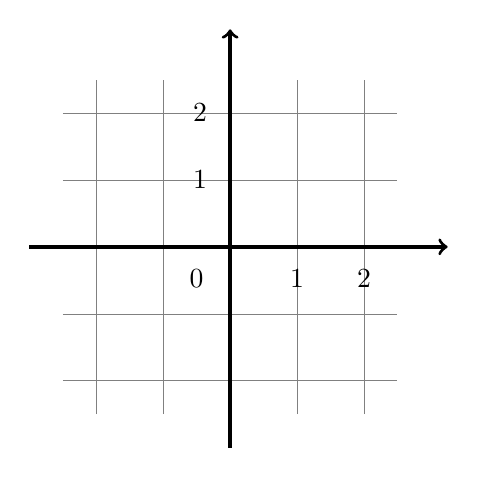
\begin{tikzpicture}[scale=0.85]
        \draw[help lines] (-2.5,-2.5) grid (2.5, 2.5);
        \draw[very thick, ->] (-3, 0) -- (3.25, 0);
        \draw[very thick, ->] (0, -3) -- (0, 3.25);
        \node[overlay, left] at (-0.2, 1) {$1$};
        \node[overlay, left] at (-0.2, 2) {$2$};
        \node[overlay, below] at (-0.5, -0.2) {$0$};
        \node[overlay, below] at (1, -0.2) {$1$};
        \node[overlay, below] at (2, -0.2) {$2$};
        \end{tikzpicture}
        \end{center}
\fi

\ifnum \Version=2
\question[2] Consider the autonomous differential equation $\displaystyle \frac{dy}{dt}= (y-k)(y+1-k^2)$.  Assume $k$ can be any real number. Draw the bifurcation diagram on the axes below. That is, plot the location of the critical points versus $k$. Please label your axes.
        \begin{center}
        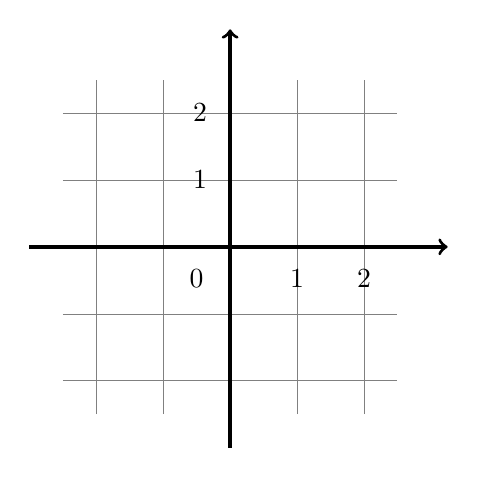
\begin{tikzpicture}[scale=0.85]
        \draw[help lines] (-2.5,-2.5) grid (2.5, 2.5);
        \draw[very thick, ->] (-3, 0) -- (3.25, 0);
        \draw[very thick, ->] (0, -3) -- (0, 3.25);
        \node[overlay, left] at (-0.2, 1) {$1$};
        \node[overlay, left] at (-0.2, 2) {$2$};
        \node[overlay, below] at (-0.5, -0.2) {$0$};
        \node[overlay, below] at (1, -0.2) {$1$};
        \node[overlay, below] at (2, -0.2) {$2$};
        \end{tikzpicture}
        \end{center}
\fi

\ifnum \Version=3
    \question[2] You do not need to show your work for this question. Consider the differential equation 
    \begin{align*}
        t^2y'' - 4ty' - 2y = 12
    \end{align*}
    The DE can be expressed in the form $\vec x\, ' = A\vec x + \vec g$, where 
    \begin{align*}
     A = \left( \hbox to 2cm{\vbox to 0.85cm{}} \right), \quad \vec g = \left( \hbox to 1.2cm{\vbox to 0.85cm{}} \right)
    \end{align*}
    Fill in the missing entries in the above to define $A$ and $\vec g$. 
\fi

\ifnum \Version=4
\question[2] Consider the autonomous differential equation $\displaystyle \frac{dy}{dt}= (y+k)(y^2-k)$.  Assume $k\ge0$. Draw the bifurcation diagram on the axes below. That is, plot the location of the critical points versus $k$. Please label your axes.
        \begin{center}
        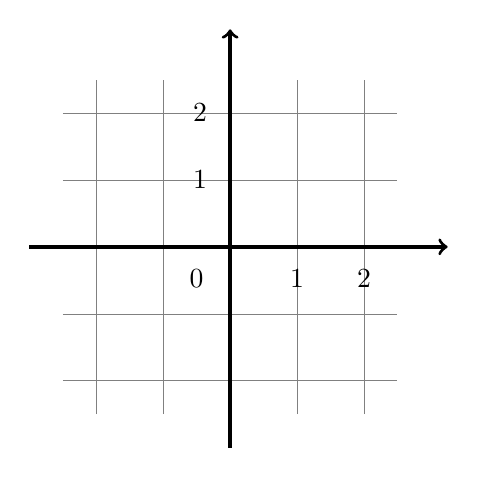
\begin{tikzpicture}[scale=0.85]
        \draw[help lines] (-2.5,-2.5) grid (2.5, 2.5);
        \draw[very thick, ->] (-3, 0) -- (3.25, 0);
        \draw[very thick, ->] (0, -3) -- (0, 3.25);
        \node[overlay, left] at (-0.2, 1) {$1$};
        \node[overlay, left] at (-0.2, 2) {$2$};
        \node[overlay, below] at (-0.5, -0.2) {$0$};
        \node[overlay, below] at (1, -0.2) {$1$};
        \node[overlay, below] at (2, -0.2) {$2$};
        \end{tikzpicture}
        \end{center}
\fi

\ifnum \Version=5
    \question[2] You do not need to show your work for this question. Consider the differential equation 
    \begin{align*}
        4y'' - t^2y' - 2ty = 12\cos(t)
    \end{align*}
    The DE can be expressed in the form $\vec x\, ' = A\vec x + \vec g$, where 
    \begin{align*}
     A = \left( \hbox to 2cm{\vbox to 0.85cm{}} \right), \quad \vec g = \left( \hbox to 1.2cm{\vbox to 0.85cm{}} \right)
    \end{align*}
    Fill in the missing entries in the above to define $A$ and $\vec g$. 
\fi




\ifnum \Version=6
\question[1] You do not need to show your work for this question. Consider the IVP below.
$$\displaystyle y' = \sqrt{4-t^2+y}, \ y(1) = 2$$   
Using the theorems we covered in lecture, fill in all of the appropriate circles below to indicate the intervals over which there must contain a unique solution to the IVP. 
\begin{itemize}
    \item[$\bigcirc$] $y \ge 4-t^2$
    \item[$\bigcirc$] $y \le 4-t^2$
    \item[$\bigcirc$] $y \le t^2-4$
    \item[$\bigcirc$] $y \ge t^2-4$
    \item[$\bigcirc$] none of the above
\end{itemize}
\ifnum \Solutions=1 {\color{DarkBlue} 
\textbf{Solutions:} the relevant theorem is below. 

    \begin{center}\begin{tikzpicture} \node [mybox](box){\begin{minipage}{0.95\textwidth} \vspace{4pt}

    If $f$ and $\frac{\partial f}{\partial y}$ are continuous over $\alpha < t < \beta$, and $\gamma < y < \delta$, which contains the point $(t_0,y_0)$, then there is a unique solution to the IVP $$y' = f(t,y), \quad y(t_0) = y_0$$ on an interval contained in $\alpha < t < \beta$. 
    
    \end{minipage}}; \node[fancytitle, rounded corners, thick, inner sep = 4pt, right=10pt] at (box.north west) {Theorem 2.4.2: Existence and Uniqueness of 1st Order Nonlinear IVP};
    \end{tikzpicture}\end{center}
    
    Taking the partial derivative with respect to $y$:
\begin{align}
    \frac{\partial f}{\partial y} &= \frac{1}{\sqrt{4-t^2+y}}\\
\end{align}
The relevant functions are 
\begin{align}
    f(t,y) &= \sqrt{4-t^2+y} \\
    \frac{\partial f}{\partial y} &= \frac{1}{\sqrt{4-t^2+y}}
\end{align}
They are real and continuous over $$4-t^2+y > 0$$ and this interval also contains $t_0 = 0$ and $y(t_0)$. So the interval over which there must contain a unique solution is $$y > t^2-4$$ 
} 
\else 
\fi
\fi 




\ifnum \Version=7
\question[1] You do not need to show your work for this question. Consider the IVP below.
$$\displaystyle (t+3)y' + \sqrt{4-t^2}\,y = t^4, \ y(1) = 9$$   
Using the theorems we covered in lecture, fill in all of the appropriate circles below to indicate the intervals over which there must contain a unique solution to the IVP. 
\begin{itemize}
    \item[$\bigcirc$] $-3 < t \le 2$
    \item[$\bigcirc$] $-2 \le t \le 2$
    \item[$\bigcirc$] $-2 \le t \le 3$    
    \item[$\bigcirc$] $-\infty \le t < -3$
    \item[$\bigcirc$] none of the above
\end{itemize}
\ifnum \Solutions=1 {\color{DarkBlue} 
\textbf{Solutions:} convert to standard form:
\begin{align}
    y' + \frac{\sqrt{4-t^2}}{t+3}\,y = \frac{t^4}{t+3}
\end{align}
The coefficients are real and continuous over $$-2\le t \le 2$$ and this interval also contains $t_0 = 1$. So the interval over which there must contain a unique solution is $-2\le t \le 2$. 
} 
\else 
\fi
\fi 



\ifnum \Version=8
\question[1] You do not need to show your work for this question. Consider the IVP below.
$$\displaystyle y' = \sqrt{4-t^2-y}, \ y(0) = 2$$   
Using the theorems we covered in lecture, fill in all of the appropriate circles below to indicate the intervals over which there must contain a unique solution to the IVP. 
\begin{itemize}
    \item[$\bigcirc$] $y \ge 4-t^2$
    \item[$\bigcirc$] $y \le 4-t^2$
    \item[$\bigcirc$] $y \le t^2-4$
    \item[$\bigcirc$] $y \ge t^2-4$
    \item[$\bigcirc$] none of the above
\end{itemize}
\ifnum \Solutions=1 {\color{DarkBlue} 
\textbf{Solutions:} partial derivative with respect to $y$:
\begin{align}
    \frac{\partial f}{\partial y} &= \frac{-1}{\sqrt{4-t^2-y}}
\end{align}
The coefficients are real and continuous over $$4-t^2-y\ge 0$$ and this interval also contains $t_0 = 0$ and $y(t_0)$. So the interval over which there must contain a unique solution is $y \le 4-t^2$. 
} 
\else 
\fi
\fi 



\ifnum \Version=9
\question[1] You do not need to show your work for this question. Consider the IVP below.
$$\displaystyle y' = \sqrt{4-t^2+y}, \ y(0) = 2$$   
Using the theorems we covered in lecture, fill in all of the appropriate circles below to indicate the intervals over which there must contain a unique solution to the IVP. 
\begin{itemize}
    \item[$\bigcirc$] $y \ge 4-t^2$
    \item[$\bigcirc$] $y \le 4-t^2$
    \item[$\bigcirc$] $y \le t^2-4$
    \item[$\bigcirc$] $y \ge t^2-4$
    \item[$\bigcirc$] none of the above
\end{itemize}
\ifnum \Solutions=1 {\color{DarkBlue} 
\textbf{Solutions:} partial derivative with respect to $y$:
\begin{align}
    \frac{\partial f}{\partial y} &= \frac{1}{\sqrt{4-t^2+y}}\\
\end{align}
The coefficients are real and continuous over $$4-t^2+y\ge 0$$ and this interval also contains $t_0 = 0$ and $y(t_0)$. So the interval over which there must contain a unique solution is $y \ge t^2-4$. 
} 
\else 
\fi
\fi 




    \ifnum \Version=6
\question[3] Consider the system $$\vec x \, ' = A\vec x, \quad A = \begin{pmatrix} -3&-4\\1&-1 \end{pmatrix}, \quad \vec x = \begin{pmatrix} x(t)\\y(t)\end{pmatrix} $$ The eigenvalues of $A$ are $\lambda = -2\pm i\sqrt 3$. Sketch the phase portrait of the system. Sketch at least two solution curves. Please indicate the direction of motion on your solution curves. Don't forget to label your axes.   

\ifnum \Solutions=1 {\color{DarkBlue} 
\textbf{Solutions:} solution curves should \textbf{spiral towards} the origin and rotate \textbf{counter clockwise}. Axes should be labelled. Ok to only draw only two solution curves. 
    \begin{center}
    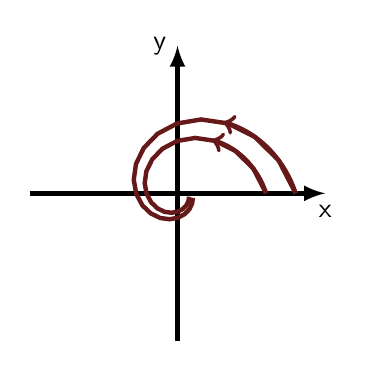
\begin{tikzpicture}[scale=0.75]
      \draw[ultra thick,->,>=latex] (-2.5,0)--(2.5,0) node[below] {x};
      \draw[ultra thick,->,>=latex] (0,-2.5)--(0,2.5) node[left] {y};      
      \draw[domain=0:6,ultra thick,samples=20,DarkRed] plot ({cos(deg(\x))*2*exp(-\x/3},{sin(deg(\x))*2*exp(-\x/3});
      \draw[domain=0:1,->,ultra thick,samples=20,DarkRed] plot ({cos(deg(\x))*2*exp(-\x/3},{sin(deg(\x))*2*exp(-\x/3});
      \draw[domain=0:6,ultra thick,samples=20,DarkRed] plot ({.75*cos(deg(\x))*2*exp(-\x/3},{.75*sin(deg(\x))*2*exp(-\x/3});
      \draw[domain=0:1,->,ultra thick,samples=20,DarkRed] plot ({.75*cos(deg(\x))*2*exp(-\x/3},{.75*sin(deg(\x))*2*exp(-\x/3});
    \end{tikzpicture}
    \end{center} 
} 
\else 
    \begin{center}
    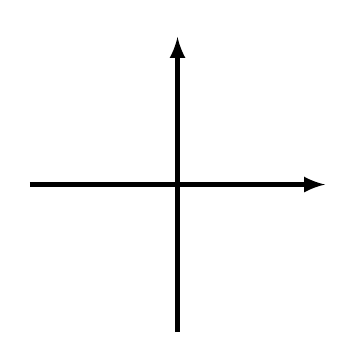
\begin{tikzpicture}[scale=0.75]
      \draw[ultra thick,->,>=latex] (-2.5,0)--(2.5,0) node[below] {};
      \draw[ultra thick,->,>=latex] (0,-2.5)--(0,2.5) node[left] {};         
    \end{tikzpicture}
    \end{center} 
\fi
\fi


\ifnum \Version=7
\question[3] Consider the system $$\vec x \, ' = A\vec x, \quad A = \begin{pmatrix} 3&2\\-5&1 \end{pmatrix}, \quad \vec x = \begin{pmatrix} x(t)\\y(t)\end{pmatrix} $$ The eigenvalues of $A$ are $\lambda = 2\pm  3i$. Sketch the phase portrait of the system. Sketch at least two solution curves. Please indicate the direction of motion on your solution curves. Don't forget to label your axes.   

\ifnum \Solutions=1 {\color{DarkBlue} 
\textbf{Solutions:} solution curves should \textbf{spiral away} from the origin and rotate \textbf{clockwise}. Axes should be labelled. Ok to only draw only two solution curves. 
\begin{center}
    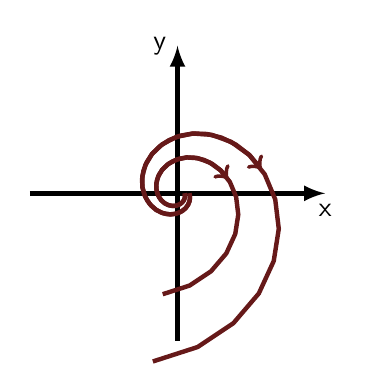
\begin{tikzpicture}[scale=0.75]
      \draw[ultra thick,->,>=latex] (-2.5,0)--(2.5,0) node[below] {x};
      \draw[ultra thick,->,>=latex] (0,-2.5)--(0,2.5) node[left] {y};      
      \draw[domain=0:8,ultra thick,samples=30,DarkRed] plot ({cos(deg(\x))*0.12*exp(\x/3)},{-sin(deg(\x))*0.12*exp(\x/3)});
      \draw[domain=0:6,->,ultra thick,samples=30,DarkRed] plot ({cos(deg(\x))*0.12*exp(\x/3)},{-sin(deg(\x))*0.12*exp(\x/3)});
      \draw[domain=0:8,ultra thick,samples=30,DarkRed] plot ({cos(deg(\x))*0.2*exp(\x/3)},{-sin(deg(\x))*0.2*exp(\x/3)});
      \draw[domain=0:6,->,ultra thick,samples=30,DarkRed] plot ({cos(deg(\x))*0.2*exp(\x/3)},{-sin(deg(\x))*0.2*exp(\x/3)});      
    \end{tikzpicture}
\end{center} 
} 
\else 
\begin{center}
    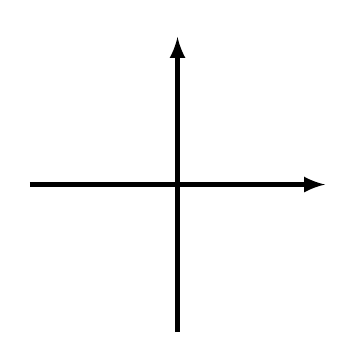
\begin{tikzpicture}[scale=0.75]
      \draw[ultra thick,->,>=latex] (-2.5,0)--(2.5,0) node[below] {};
      \draw[ultra thick,->,>=latex] (0,-2.5)--(0,2.5) node[left] {};         
    \end{tikzpicture}
\end{center} 
\fi
\fi






\ifnum \Version=8
\question[3] Consider the system $$\vec x \, ' = A\vec x, \quad A = \begin{pmatrix} -3&-4\\1&-1 \end{pmatrix}, \quad \vec x = \begin{pmatrix} x(t)\\y(t)\end{pmatrix} $$ The eigenvalues of $A$ are $\lambda = -2\pm i\sqrt 3$. Sketch the phase portrait of the system. Sketch at least two solution curves. Please indicate the direction of motion on your solution curves. Don't forget to label your axes.   

\ifnum \Solutions=1 {\color{DarkBlue} 
\textbf{Solutions:} solution curves should spiral towards center and rotate counter clockwise. Axes should be labelled. Ok to only draw only two solution curves. 
    \begin{center}
    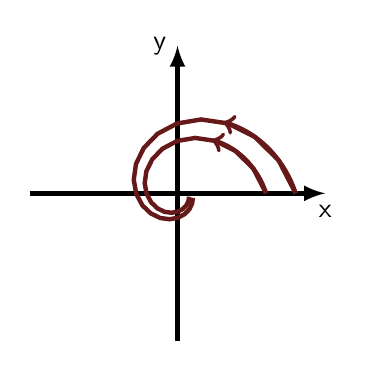
\begin{tikzpicture}[scale=0.75]
      \draw[ultra thick,->,>=latex] (-2.5,0)--(2.5,0) node[below] {x};
      \draw[ultra thick,->,>=latex] (0,-2.5)--(0,2.5) node[left] {y};      
      \draw[domain=0:6,ultra thick,samples=20,DarkRed] plot ({cos(deg(\x))*2*exp(-\x/3},{sin(deg(\x))*2*exp(-\x/3});
      \draw[domain=0:1,->,ultra thick,samples=20,DarkRed] plot ({cos(deg(\x))*2*exp(-\x/3},{sin(deg(\x))*2*exp(-\x/3});
      \draw[domain=0:6,ultra thick,samples=20,DarkRed] plot ({.75*cos(deg(\x))*2*exp(-\x/3},{.75*sin(deg(\x))*2*exp(-\x/3});
      \draw[domain=0:1,->,ultra thick,samples=20,DarkRed] plot ({.75*cos(deg(\x))*2*exp(-\x/3},{.75*sin(deg(\x))*2*exp(-\x/3});
    \end{tikzpicture}
    \end{center} 
} 
\else 
    \begin{center}
    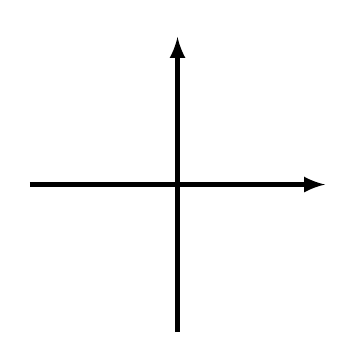
\begin{tikzpicture}[scale=0.75]
      \draw[ultra thick,->,>=latex] (-2.5,0)--(2.5,0) node[below] {};
      \draw[ultra thick,->,>=latex] (0,-2.5)--(0,2.5) node[left] {};         
    \end{tikzpicture}
    \end{center} 
\fi
\fi




\ifnum \Version=9
\question[3] Consider the system $$\vec x \, ' = A\vec x, \quad A = \begin{pmatrix} 1&-4\\1&3 \end{pmatrix}, \quad \vec x = \begin{pmatrix} x(t)\\y(t)\end{pmatrix} $$ The eigenvalues of $A$ are $\lambda = 2\pm i\sqrt 3$. Sketch the phase portrait of the system. Sketch at least two solution curves. Please indicate the direction of motion on your solution curves. Don't forget to label your axes.   

\ifnum \Solutions=1 {\color{DarkBlue} 
\textbf{Solutions:} solution curves should spiral away from the origin and rotate counter clockwise. Axes should be labelled. Ok to only draw only two solution curves. 
    \begin{center}
    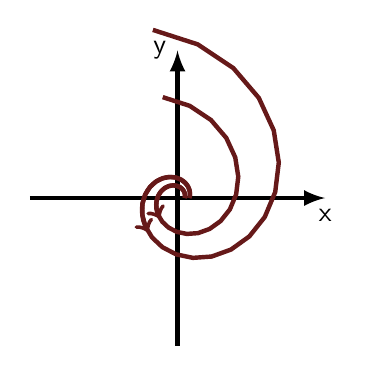
\begin{tikzpicture}[scale=0.75]
      \draw[ultra thick,->,>=latex] (-2.5,0)--(2.5,0) node[below] {x};
      \draw[ultra thick,->,>=latex] (0,-2.5)--(0,2.5) node[left] {y};      
      \draw[domain=0:8,ultra thick,samples=30,DarkRed] plot ({cos(deg(\x))*0.12*exp(\x/3)},{sin(deg(\x))*0.12*exp(\x/3)});
      \draw[domain=0:4,->,ultra thick,samples=30,DarkRed] plot ({cos(deg(\x))*0.12*exp(\x/3)},{sin(deg(\x))*0.12*exp(\x/3)});
      \draw[domain=0:8,ultra thick,samples=30,DarkRed] plot ({cos(deg(\x))*0.2*exp(\x/3)},{sin(deg(\x))*0.2*exp(\x/3)});
      \draw[domain=0:4,->,ultra thick,samples=30,DarkRed] plot ({cos(deg(\x))*0.2*exp(\x/3)},{sin(deg(\x))*0.2*exp(\x/3)});      
    \end{tikzpicture}
    \end{center} 
} 
\else 
    \begin{center}
    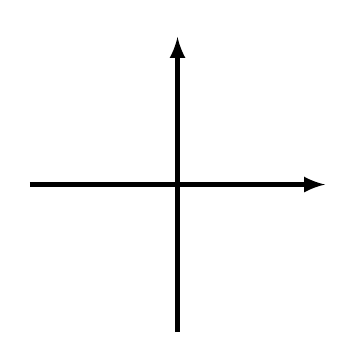
\begin{tikzpicture}[scale=0.75]
      \draw[ultra thick,->,>=latex] (-2.5,0)--(2.5,0) node[below] {};
      \draw[ultra thick,->,>=latex] (0,-2.5)--(0,2.5) node[left] {};         
    \end{tikzpicture}
    \end{center} 
\fi
\fi



    
\ifnum \Version>5
\question[3] A tank originally contains 50 L of water with 6 kg of salt. Water containing $\frac{1}{20}$ kg of salt per litre is entering at a rate of 4 L/hour, and the well-stirred solution in the tank is leaving at 1 L/hour. 

\begin{parts}
    \part Write down an IVP for $V(t)$, which is the amount of fluid in the tank at time $t$. You do not need to solve your IVP. 
    
    \ifnum \Solutions=1 {\color{DarkBlue} 
        The volume of fluid in the tank is
        $$V = 50 + 3t$$
        By differentiating, the IVP for $V(t)$ is
        $$\frac{dV}{dt} = 3, \quad V(0) = 50$$
        }
    \else
    \vspace{6cm}
    \fi
    
    \part Write down an IVP for $Q(t)$, for the amount of salt in the tank. You do not need to solve the IVP. 
    
    \ifnum \Solutions=1 {\color{DarkBlue} 
        The DE is
        \begin{align}
            \frac{dQ}{dt} &= \left( \text{rate salt coming in} \right) - \left( \text{rate of salt going out} \right) \\
            \frac{dQ}{dt} &= 4\cdot \frac{1}{20} - \frac{Q}{V}
        \end{align}
        The IVP is
        \begin{align}
            \frac{dQ}{dt} &= \frac{1}{5} - \frac{Q}{50+3t}, \quad Q(0) = 6
        \end{align}        
        }
        \fi
    \fi
    
\end{parts}


        

    \newpage        
    \newpage 
\ifnum \Version=1  
\question[4] Solve the initial value problem and solve for $y$ to obtain an explicit expression for $y$ in terms of $t$. Please show your work.
$$\displaystyle t\,\frac{dy}{dt} = \frac{\cos(t)}{t^2} - 3y, \quad y(\pi) = 2, \quad t > 0$$.
\fi

\ifnum \Version=2
\question[4] Solve the initial value problem and solve for $y$ to obtain an explicit expression for $y$ in terms of $t$. Please show your work.
$$\displaystyle \frac{dy}{dt} = 12e^{3t}e^{-2y}, \quad y(0) = 2, \quad t \ge 0$$.
\fi

\ifnum \Version=3
\question[4] Solve the initial value problem and solve for $y$ to obtain an explicit expression for $y$ in terms of $t$. Please show your work.
$$\displaystyle t\,\frac{dy}{dt} + 3y =  36 t^{-2}e^{-t}, \ y(1) = 0, \quad t > 0$$.
\fi   

\ifnum \Version=4
\question[4] Solve the initial value problem and solve for $y$ to obtain an expression for $y$ in terms of $t$. Please show your work.
$$\displaystyle \frac{dy}{dt} = \frac{16e^{2t}}{y}, \quad y(1) = 2, \quad t > 0$$.
\fi

\ifnum \Version=5
\question[4] Solve the initial value problem and solve for $y$ to obtain an explicit expression for $y$ in terms of $t$. Please show your work.
$$\displaystyle t\,\frac{dy}{dt} + 2y =  36 t^{-1}e^{t}, \ y(1) = 2e, \quad t > 0$$.
\fi   



\ifnum \Version=6
\question[4] 
Solve the initial value problem and solve for $y$ to obtain an explicit expression for $y$ in terms of $t$. Please show your work.
$$\displaystyle t\,\frac{dy}{dt} + 4y =  24 t^{-3}e^{2t}, \ y(1) = 2, \quad t > 0$$.

\ifnum \Solutions=1 {\color{DarkBlue} 
\textbf{Solutions:}
To solve the differential equation \( t y' + 4 y = 24 t^{-3} e^{2t} \) with the initial condition \( y(1) = 2 \), we can follow these steps.
\begin{enumerate}
    \item Rewrite the DE in standard form:
   \[ y' + \frac{4}{t} y = 24 t^{-4} e^{2t} \]
   \item Integrating factor:
   \[ \mu(t) = e^{\int \frac{4}{t} \, dt} = e^{4 \ln |t|} = t^4 \]
   \item Multiply both sides of the differential equation by the integrating factor:
   \begin{align*}
       t^4 y' + 4 t^3 y &= 24 e^{2t} \\
       \frac{d}{dt} (t^4 y) &= 24 e^{2t}
   \end{align*} 
   \item Integrate both sides with respect to \( t \) and solve for $y$:
   \begin{align}
       t^4 y &= \int 24 e^{2t} \, dt + C \\
       t^4 y &= 12 e^{2t} + C \\
        y &= \frac{12 e^{2t} + C}{t^4} 
   \end{align} 
   \item Apply the initial condition \( y(1) = 2 \):
   \[ 2 = \frac{12 e^{2 \cdot 1} + C}{1^4} \]
   \[ 2 = 12 e^2 + C \]
   \[ C = 2 - 12 e^2 \]
   \item Substitute \( C \) back into the solution:
   \[ y = \frac{12 e^{2t} + 2 - 12 e^2}{t^4} \]
\end{enumerate}
} 
\else 
\newpage
\fi
\fi   





\ifnum \Version=7
\question[4] 
Solve the initial value problem and solve for $y$ to obtain an explicit expression for $y$ in terms of $t$. Please show your work.
$$\displaystyle t\,\frac{dy}{dt} + 5y =  20 t^{-4}e^{2t}, \ y(1) = e^2, \quad t > 0$$.

\ifnum \Solutions=1 {\color{DarkBlue} 
\textbf{Solutions:}
To solve the differential equation \( t y' + 5 y = 20 t^{-3} e^{2t} \) with the initial condition \( y(1) = 2 \), we can follow these steps.
\begin{enumerate}
    \item Rewrite the DE in standard form:
   \[ y' + \frac{5}{t} y = 20 t^{-4} e^{2t} \]
   \item Integrating factor:
   \[ \mu(t) = e^{\int \frac{5}{t} \, dt} = e^{5 \ln |t|} = t^5 \]
   \item Multiply both sides of the differential equation by the integrating factor:
   \begin{align*}
       t^5 y' + 5 t^4 y &= 20 e^{2t} \\
       \frac{d}{dt} (t^5 y) &= 20 e^{2t}
   \end{align*} 
   \item Integrate both sides with respect to \( t \) and solve for $y$:
   \begin{align}
       t^5 y &= \int 20 e^{2t} \, dt + C \\
       t^5 y &= 10 e^{2t} + C \\
        y &= \frac{10 e^{2t} + C}{t^5} 
   \end{align} 
   \item Apply the initial condition \( y(1) = e^2 \):
   \[ e^2 = \frac{10 e^{2 \cdot 1} + C}{1^5} \]
   \[ e^2 = 10 e^2 + C \]
   \[ C = - 9 e^2 \]
   \item Substitute \( C \) back into the solution:
   \[ y = \frac{10 e^{2t} - 9 e^2}{t^5} \]
\end{enumerate}
} 
\else 
\newpage
\fi
\fi   






\ifnum \Version=8
\question[4] 
Solve the initial value problem and solve for $y$ to obtain an explicit expression for $y$ in terms of $t$. Please show your work.
$$\displaystyle t\,\frac{dy}{dt} + 6y =  24 t^{-5}e^{4t}, \ y(1) = 8e^4, \quad t > 0$$.

\ifnum \Solutions=1 {\color{DarkBlue} 
\textbf{Solutions:}
To solve the DE with the given initial condition we can follow these steps.
\begin{enumerate}
    \item Rewrite the DE in standard form:
   \[ y' + \frac{6}{t} y = 24 t^{-6} e^{4t} \]
   \item Integrating factor:
   \[ \mu(t) = e^{\int \frac{6}{t} \, dt} = e^{6 \ln |t|} = t^6 \]
   \item Multiply both sides of the differential equation by the integrating factor:
   \begin{align*}
       t^6 y' + 6 t^5 y &= 24 e^{4t} \\
       \frac{d}{dt} (t^6 y) &= 24 e^{4t}
   \end{align*} 
   \item Integrate both sides with respect to \( t \) and solve for $y$:
   \begin{align}
       t^6 y &= \int 24 e^{4t} \, dt + C \\
       t^6 y &= 6 e^{4t} + C \\
        y &= \frac{6 e^{4t} + C}{t^6} 
   \end{align} 
   \item Apply the initial condition:
   \[ 8e^4 = \frac{6 e^{4 \cdot 1} + C}{1^5} \]
   \[ 8e^4 = 6 e^4 + C \]
   \[ C = 2 e^4 \]
   \item Substitute \( C \) back into the solution:
   \[ y = \frac{6 e^{4t} +2 e^4}{t^6} \]
\end{enumerate}
} 
\else 
\newpage
\fi
\fi   



\ifnum \Version=9
\question[4] 
Solve the initial value problem and solve for $y$ to obtain an explicit expression for $y$ in terms of $t$. Please show your work.
$$\displaystyle t\,\frac{dy}{dt} + 5y =  20 t^{-4}e^{2t}, \ y(1) = e^2, \quad t > 0$$.

\ifnum \Solutions=1 {\color{DarkBlue} 
\textbf{Solutions:}
To solve the differential equation \( t y' + 5 y = 20 t^{-3} e^{2t} \) with the initial condition \( y(1) = 2 \), we can follow these steps.
\begin{enumerate}
    \item Rewrite the DE in standard form:
   \[ y' + \frac{5}{t} y = 20 t^{-4} e^{2t} \]
   \item Integrating factor:
   \[ \mu(t) = e^{\int \frac{5}{t} \, dt} = e^{5 \ln |t|} = t^5 \]
   \item Multiply both sides of the differential equation by the integrating factor:
   \begin{align*}
       t^5 y' + 5 t^4 y &= 20 e^{2t} \\
       \frac{d}{dt} (t^5 y) &= 20 e^{2t}
   \end{align*} 
   \item Integrate both sides with respect to \( t \) and solve for $y$:
   \begin{align}
       t^5 y &= \int 20 e^{2t} \, dt + C \\
       t^5 y &= 10 e^{2t} + C \\
        y &= \frac{10 e^{2t} + C}{t^5} 
   \end{align} 
   \item Apply the initial condition \( y(1) = e^2 \):
   \[ e^2 = \frac{10 e^{2 \cdot 1} + C}{1^5} \]
   \[ e^2 = 10 e^2 + C \]
   \[ C = - 9 e^2 \]
   \item Substitute \( C \) back into the solution:
   \[ y = \frac{10 e^{2t} - 9 e^2}{t^5} \]
\end{enumerate}
} 
\else 
\newpage
\fi
\fi   
        
    \newpage 

\ifnum \Version=1  
\question[7] Consider the system $$\vec x \, ' = A\vec x, \quad A = \begin{pmatrix} 0&3\\5&2 \end{pmatrix}, \quad \vec x = \begin{pmatrix} x(t)\\y(t)\end{pmatrix} $$.
\begin{parts}
    \part Determine the eigenvalues of $A$. Please show your work. \vspace{5cm}
    \part Determine the eigenvectors of $A$. Please show your work. \vspace{7cm}
    \part Sketch the phase portrait of the system on the axes below. Please indicate the direction of motion on your solution curves and draw the eigenspaces corresponding to real eigenvalues (if any). Please also label your axes. 
    \begin{center}
    \begin{tikzpicture}[scale=0.85]
    \draw[very thick, ->] (-3, 0) -- (3.25, 0);
    \draw[very thick, ->] (0, -3) -- (0, 3.25);
    \end{tikzpicture}
    \end{center}
\end{parts}
\fi

\ifnum \Version=2
\question[7] Consider the system $$\vec x \, ' = A\vec x, \quad A = \begin{pmatrix} 4&3\\3&-4 \end{pmatrix}, \quad \vec x = \begin{pmatrix} x(t)\\y(t)\end{pmatrix} $$.
\begin{parts}
    \part Determine the eigenvalues of $A$. Please show your work. \vspace{5cm}
    \part Determine the eigenvectors of $A$. Please show your work. \vspace{7cm}
    \part Sketch the phase portrait of the system on the axes below. Please indicate the direction of motion on your solution curves and draw the eigenspaces corresponding to real eigenvalues (if any). Please also label your axes. 
    \begin{center}
    \begin{tikzpicture}[scale=0.85]
    \draw[very thick, ->] (-3, 0) -- (3.25, 0);
    \draw[very thick, ->] (0, -3) -- (0, 3.25);
    \end{tikzpicture}
    \end{center}
\end{parts}
\fi

\ifnum \Version=3
\question[7] Consider the system $$\vec x \, ' = A\vec x, \quad A = \begin{pmatrix} 5&4\\-3&-3 \end{pmatrix}, \quad \vec x = \begin{pmatrix} x(t)\\y(t)\end{pmatrix} $$.
\begin{parts}
    \part Determine the eigenvalues of $A$. Please show your work. \vspace{5cm}
    \part Determine the eigenvectors of $A$. Please show your work. \vspace{7cm}
    \part Sketch the phase portrait of the system on the axes below. Please indicate the direction of motion on your solution curves and draw the eigenspaces corresponding to real eigenvalues (if any). Please also label your axes. 
    \begin{center}
    \begin{tikzpicture}[scale=0.85]
    \draw[very thick, ->] (-3, 0) -- (3.25, 0);
    \draw[very thick, ->] (0, -3) -- (0, 3.25);
    \end{tikzpicture}
    \end{center}
\end{parts}
\fi

\ifnum \Version=4
\question[7] Consider the system $$\vec x \, ' = A\vec x, \quad A = \begin{pmatrix} 3&4\\-3&-5 \end{pmatrix}, \quad \vec x = \begin{pmatrix} x(t)\\y(t)\end{pmatrix} $$.
\begin{parts}
    \part Determine the eigenvalues of $A$. Please show your work. \vspace{5cm}
    \part Determine the eigenvectors of $A$. Please show your work. \vspace{7cm}
    \part Sketch the phase portrait of the system on the axes below. Please indicate the direction of motion on your solution curves and draw the eigenspaces corresponding to real eigenvalues (if any). Please also label your axes. 
    \begin{center}
    \begin{tikzpicture}[scale=0.85]
    \draw[very thick, ->] (-3, 0) -- (3.25, 0);
    \draw[very thick, ->] (0, -3) -- (0, 3.25);
    \end{tikzpicture}
    \end{center}
\end{parts}
\fi

\ifnum \Version=5
\question[7] Consider the system $$\vec x \, ' = A\vec x, \quad A = \begin{pmatrix} 4&4\\-3&-4 \end{pmatrix}, \quad \vec x = \begin{pmatrix} x(t)\\y(t)\end{pmatrix} $$.
\begin{parts}
    \part Determine the eigenvalues of $A$. Please show your work. \vspace{5cm}
    \part Determine the eigenvectors of $A$. Please show your work. \vspace{7cm}
    \part Sketch the phase portrait of the system on the axes below. Please indicate the direction of motion on your solution curves and draw the eigenspaces corresponding to real eigenvalues (if any). Please also label your axes. 
    \begin{center}
    \begin{tikzpicture}[scale=0.85]
    \draw[very thick, ->] (-3, 0) -- (3.25, 0);
    \draw[very thick, ->] (0, -3) -- (0, 3.25);
    \end{tikzpicture}
    \end{center}
\end{parts}
\fi



\ifnum \Version=6
    \question[6] Consider the IVP $$\vec x \, ' = A\vec x, \quad A = \begin{pmatrix} -1&3\\3&-1 \end{pmatrix}, \quad \vec x = \begin{pmatrix} x(t)\\y(t)\end{pmatrix}, \quad \vec x(0) = \begin{pmatrix} 2\\2 \end{pmatrix}$$ The eigenvalues of $A$ are $\lambda_1 = -4$ and $\lambda_2 = 2$. 
    \begin{parts}
        \part Determine the eigenvectors of $A$. Please show your work. 
        
        \ifnum \Solutions=1 {\color{DarkBlue} 
        \textbf{Solutions:}
        For $\lambda_1$:
        \begin{align}
            A - \lambda_1 I = \begin{pmatrix} 3&3\\3&3\end{pmatrix} \ \Rightarrow \ v_1 = \begin{pmatrix} -1\\1 \end{pmatrix}
        \end{align}
        For $\lambda_2$:
        \begin{align}
            A - \lambda_2 I = \begin{pmatrix} -3&3\\3&-3\end{pmatrix} \ \Rightarrow \ v_2 = \begin{pmatrix} 1\\1 \end{pmatrix}
        \end{align}    
        } 
        \else 
            \vspace{6cm}   
        \fi        
        \part Use the given eigenvalues and the eigenvectors that you calculated in part (a) to solve the IVP.  
        
        \ifnum \Solutions=1 {\color{DarkBlue} 
        \textbf{Solutions:} the general solution to the DE is:
        $$\vec x = c_1 e^{-4t}\begin{pmatrix} -1\\1\end{pmatrix} + c_2e^{2t} \begin{pmatrix} 1\\1\end{pmatrix}$$
        Use initial condition:
        \begin{align}
            \begin{pmatrix} 2\\2\end{pmatrix} &= c_1\begin{pmatrix}-1\\1 \end{pmatrix}+ c_2 \begin{pmatrix} 1\\1\end{pmatrix} \ \Rightarrow \ c_1 = 0, c_2 = 2 \ \Rightarrow \ 
            \vec x (t) = 2e^{2t} \begin{pmatrix} 1\\1\end{pmatrix}
        \end{align}
        } 
        \else 
        \vspace{7cm}
    \fi
    \part Sketch the phase portrait of the system on the axes below. Please indicate the direction of motion on your solution curves and draw the eigenspaces corresponding to real eigenvalues (if any). Please also label your axes. 
    
    \ifnum \Solutions=1 {\color{DarkBlue} 
    \textbf{Solutions:}
        \begin{center}
        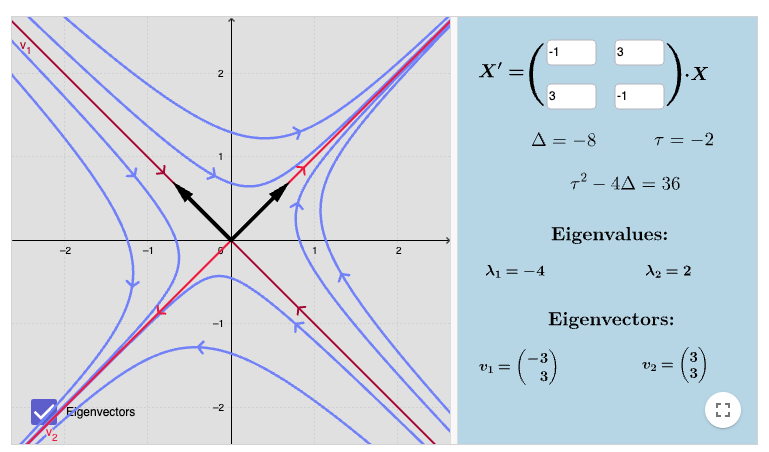
\includegraphics[width=5in]{Images/ImgPhasePlane1331.png}
        \end{center}         
    } 
    \else 
        \begin{center}
        \begin{tikzpicture}[scale=0.85]
        \draw[very thick, ->] (-3, 0) -- (3.25, 0);
        \draw[very thick, ->] (0, -3) -- (0, 3.25);
        \end{tikzpicture}
        \end{center}    
    \fi    

\end{parts}
\fi





\ifnum \Version=7
    \question[6] Consider the IVP $$\vec x \, ' = A\vec x, \quad A = \begin{pmatrix} 0&3\\3&8 \end{pmatrix}, \quad \vec x = \begin{pmatrix} x(t)\\y(t)\end{pmatrix}, \quad \vec x(0) = \begin{pmatrix} -3\\1 \end{pmatrix}$$ The eigenvalues of $A$ are $\lambda_1 = -1$ and $\lambda_2 = 9$. 
    \begin{parts}
        \part Determine the eigenvectors of $A$. Please show your work. 
        
        \ifnum \Solutions=1 {\color{DarkBlue} 
        \textbf{Solutions:}
        For $\lambda_1$:
        \begin{align}
            A - \lambda_1 I = \begin{pmatrix} 1&3\\3&9\end{pmatrix} \ \Rightarrow \ v_1 = \begin{pmatrix} -3\\1 \end{pmatrix}
        \end{align}
        For $\lambda_2$:
        \begin{align}
            A - \lambda_2 I = \begin{pmatrix} -9&3\\3&-1\end{pmatrix} \ \Rightarrow \ v_2 = \begin{pmatrix} 1\\3 \end{pmatrix}
        \end{align}    
        } 
        \else 
            \vspace{6cm}   
        \fi        
        \part Use the given eigenvalues and the eigenvectors that you calculated in part (a) to solve the IVP.  
        
        \ifnum \Solutions=1 {\color{DarkBlue} 
        \textbf{Solutions:} the general solution to the DE is:
        $$\vec x = c_1 e^{-t}\begin{pmatrix} -3\\1\end{pmatrix} + c_2e^{9t} \begin{pmatrix} 1\\3\end{pmatrix}$$
        Use initial condition:
        \begin{align}
            \begin{pmatrix} -3\\1\end{pmatrix} &= c_1\begin{pmatrix}-3\\1 \end{pmatrix}+ c_2 \begin{pmatrix} 1\\3\end{pmatrix} \ \Rightarrow \ c_1 = 1, c_2 = 0 \ \Rightarrow \ 
            \vec x (t) = e^{-t} \begin{pmatrix} -3\\1\end{pmatrix}
        \end{align}
        } 
        \else 
        \vspace{7cm}
    \fi
    \part Sketch the phase portrait of the system on the axes below. Please indicate the direction of motion on your solution curves and draw the eigenspaces corresponding to real eigenvalues (if any). Please also label your axes. 
    
    \ifnum \Solutions=1 {\color{DarkBlue} 
    \textbf{Solutions:}
        \begin{center}
        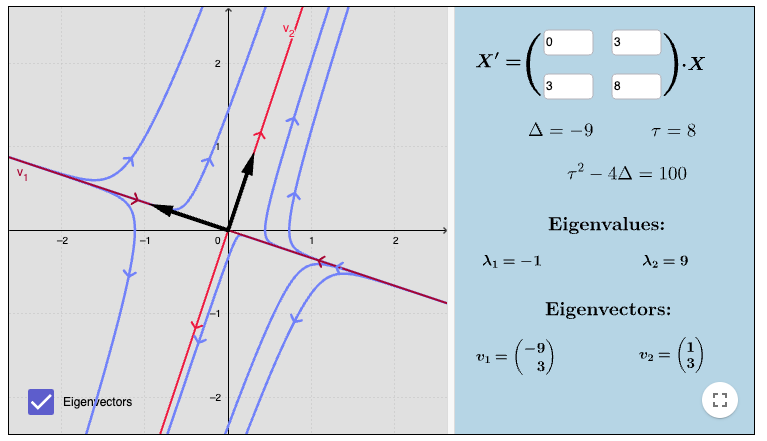
\includegraphics[width=5in]{Images/ImgPhasePlane0338.png}
        \end{center}         
    } 
    \else 
        \begin{center}
        \begin{tikzpicture}[scale=0.85]
        \draw[very thick, ->] (-3, 0) -- (3.25, 0);
        \draw[very thick, ->] (0, -3) -- (0, 3.25);
        \end{tikzpicture}
        \end{center}    
    \fi    

\end{parts}
\fi








\ifnum \Version=8
    \question[6] Consider the IVP $$\vec x \, ' = A\vec x, \quad A = \begin{pmatrix} -1&3\\3&7 \end{pmatrix}, \quad \vec x = \begin{pmatrix} x(t)\\y(t)\end{pmatrix}, \quad \vec x(0) = \begin{pmatrix} 1\\3 \end{pmatrix}$$ The eigenvalues of $A$ are $\lambda_1 = -2$ and $\lambda_2 = 8$. 
    \begin{parts}
        \part Determine the eigenvectors of $A$. Please show your work. 
        
        \ifnum \Solutions=1 {\color{DarkBlue} 
        \textbf{Solutions:}
        For $\lambda_1$:
        \begin{align}
            A - \lambda_1 I = \begin{pmatrix} 1&3\\3&9\end{pmatrix} \ \Rightarrow \ v_1 = \begin{pmatrix} -3\\1 \end{pmatrix}
        \end{align}
        For $\lambda_2$:
        \begin{align}
            A - \lambda_2 I = \begin{pmatrix} -9&3\\3&-1\end{pmatrix} \ \Rightarrow \ v_2 = \begin{pmatrix} 1\\3 \end{pmatrix}
        \end{align}    
        } 
        \else 
            \vspace{6cm}   
        \fi        
        \part Use the given eigenvalues and the eigenvectors that you calculated in part (a) to solve the IVP.  
        
        \ifnum \Solutions=1 {\color{DarkBlue} 
        \textbf{Solutions:} the general solution to the DE is:
        $$\vec x = c_1 e^{-4t}\begin{pmatrix} -1\\1\end{pmatrix} + c_2e^{2t} \begin{pmatrix} 1\\1\end{pmatrix}$$
        Use initial condition:
        \begin{align}
            \begin{pmatrix} 1\\3\end{pmatrix} &= c_1\begin{pmatrix}-3\\1 \end{pmatrix}+ c_2 \begin{pmatrix} 1\\3\end{pmatrix} \ \Rightarrow \ c_1 = 0, c_2 = 1 \ \Rightarrow \ 
            \vec x (t) = e^{8t} \begin{pmatrix} 1\\3\end{pmatrix}
        \end{align}
        } 
        \else 
        \vspace{7cm}
    \fi
    \part Sketch the phase portrait of the system on the axes below. Please indicate the direction of motion on your solution curves and draw the eigenspaces corresponding to real eigenvalues (if any). Please also label your axes. 
    
    \ifnum \Solutions=1 {\color{DarkBlue} 
    \textbf{Solutions:}
        \begin{center}
        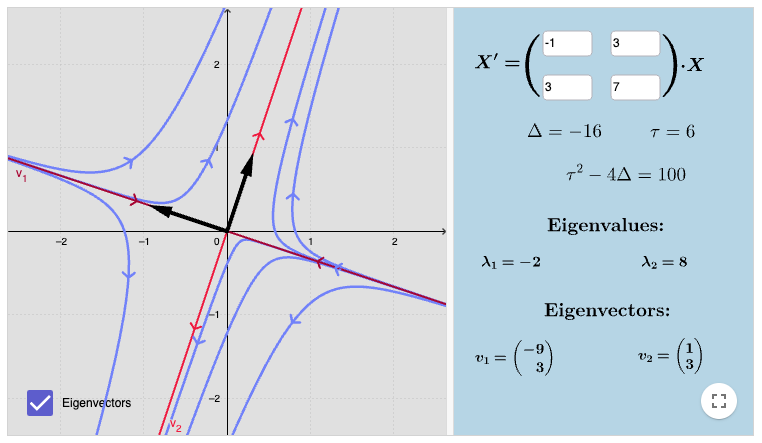
\includegraphics[width=5in]{Images/ImgPhasePlane1337.png}
        \end{center}         
    } 
    \else 
        \begin{center}
        \begin{tikzpicture}[scale=0.85]
        \draw[very thick, ->] (-3, 0) -- (3.25, 0);
        \draw[very thick, ->] (0, -3) -- (0, 3.25);
        \end{tikzpicture}
        \end{center}    
    \fi    

\end{parts}
\fi








\ifnum \Version=9
    \question[6] Consider the IVP $$\vec x \, ' = A\vec x, \quad A = \begin{pmatrix} -2&3\\3&-2 \end{pmatrix}, \quad \vec x = \begin{pmatrix} x(t)\\y(t)\end{pmatrix}, \quad \vec x(0) = \begin{pmatrix} 2\\2 \end{pmatrix}$$ The eigenvalues of $A$ are $\lambda_1 = -5$ and $\lambda_2 = 1$. 
    \begin{parts}
        \part Determine the eigenvectors of $A$. Please show your work. 
        
        \ifnum \Solutions=1 {\color{DarkBlue} 
        \textbf{Solutions:}
        For $\lambda_1$:
        \begin{align}
            A - \lambda_1 I = \begin{pmatrix} 3&3\\3&3\end{pmatrix} \ \Rightarrow \ v_1 = \begin{pmatrix} -1\\1 \end{pmatrix}
        \end{align}
        For $\lambda_2$:
        \begin{align}
            A - \lambda_2 I = \begin{pmatrix} -3&3\\3&-3\end{pmatrix} \ \Rightarrow \ v_2 = \begin{pmatrix} 1\\1 \end{pmatrix}
        \end{align}    
        } 
        \else 
            \vspace{6cm}   
        \fi        
        \part Use the given eigenvalues and the eigenvectors that you calculated in part (a) to solve the IVP.  
        
        \ifnum \Solutions=1 {\color{DarkBlue} 
        \textbf{Solutions:} the general solution to the DE is:
        $$\vec x = c_1 e^{-5t}\begin{pmatrix} -1\\1\end{pmatrix} + c_2e^{t} \begin{pmatrix} 1\\1\end{pmatrix}$$
        Use initial condition:
        \begin{align}
            \begin{pmatrix} 2\\2\end{pmatrix} &= c_1\begin{pmatrix}-1\\1 \end{pmatrix}+ c_2 \begin{pmatrix} 1\\1\end{pmatrix} \ \Rightarrow \ c_1 = 0, c_2 = 2 \ \Rightarrow \ 
            \vec x (t) = 2e^{t} \begin{pmatrix} 1\\1\end{pmatrix}
        \end{align}
        } 
        \else 
        \vspace{7cm}
    \fi
    \part Sketch the phase portrait of the system on the axes below. Please indicate the direction of motion on your solution curves and draw the eigenspaces corresponding to real eigenvalues (if any). Please also label your axes. 
    
    \ifnum \Solutions=1 {\color{DarkBlue} 
    \textbf{Solutions:}
        \begin{center}
        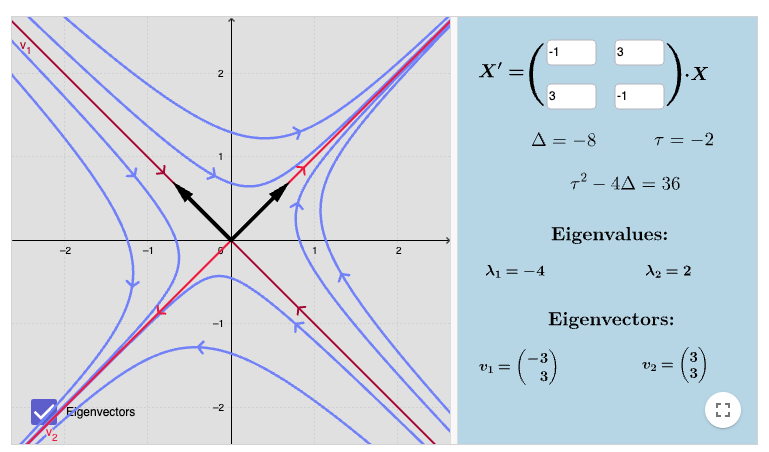
\includegraphics[width=5in]{Images/ImgPhasePlane1331.png}
        \end{center}         
    } 
    \else 
        \begin{center}
        \begin{tikzpicture}[scale=0.85]
        \draw[very thick, ->] (-3, 0) -- (3.25, 0);
        \draw[very thick, ->] (0, -3) -- (0, 3.25);
        \end{tikzpicture}
        \end{center}    
    \fi    

\end{parts}
\fi
    \ifnum \Version=1  
\question[8] Consider the differential equation $\displaystyle \frac{dy}{dt}= (y-2)(y-4k), \ k > 2$. The variable $y$ is a real function of $t$. Assume $y \in  \mathbb R$ and $t \ge 0$.
\fi
\ifnum \Version=2  
\question[8] Consider the differential equation $\displaystyle \frac{dy}{dt}= y^2-9$. The variable $y$ is a real function of $t$. Assume $y \in  \mathbb R$ and $t \ge 0$.
\fi 
\ifnum \Version=3
\question[8] Consider the differential equation $\displaystyle \frac{dy}{dt}= (y-1)(y+2)$. The variable $y$ is a real function of $t$. Assume $y \in  \mathbb R$ and $t \ge 0$.
\fi 
\ifnum \Version=4
\question[8] Consider the differential equation $\displaystyle \frac{dy}{dt}= y^2-4$. The variable $y$ is a real function of $t$. Assume $y \in  \mathbb R$ and $t \ge 0$.
\fi 
\ifnum \Version=5
\question[8] Consider the differential equation $\displaystyle \frac{dy}{dt}= (y+2)(y-3)$. The variable $y$ is a real function of $t$. Assume $y \in  \mathbb R$ and $t \ge 0$.
\fi 

\ifnum \Version<6
\begin{parts}
\part State the critical points of the differential equation.\vspace{1cm}
\part Draw the phase line, and determine whether the critical points (if any) are stable, semi-stable, or unstable.
\vspace{4cm}
\part Determine where $y$ is concave up and where $y$ is concave down for all $y \in \mathbb R$.  Show your work.
\vspace{7cm}
\part Use your results from parts A, B, and C to sketch several solution curves in the $ty$-plane for $y \in \mathbb R$ and $t \ge 0$. Clearly indicate the critical points and the points where the concavity changes. Please label your axes.     
\end{parts}
\fi


\ifnum \Version>5
\question[4] Consider the DE $\displaystyle \dydt = (y-4)(y-8)=y^2-12y+32$. Determine the values of $y$ where the solution curves are concave up and where the curves are concave down. Please show your work. 
\ifnum \Solutions=1 {\color{DarkBlue} 
    \text{Solutions:} Setting $y'=0$ we find that the equilibrium points are $y = 4, 6.$ And if $f(y) = y'$, then $$\dydtt = \dfdy \, \dydt$$ Also 
    $$\dfdy = \ddy\left(y^2-12y+32)\right) = 2y-12 = 2(y-6)$$
    So $df/dy = 0$ when $y=6$. There may be inflection points where either (or both) $df/dy$ and $dy/dt$ are zero. So there could be inflection points at $$y = 4, \ y = 8$$ A table will help determine concavity. When both derivatives have the same sign, the solutions are concave up, and when they have opposite signs the solutions are concave down. 
    \begin{center}            
        \renewcommand{\arraystretch}{1.4}
        \begin{tabular}{c|cccc} 
        $ y $ & $ (-\infty,4) $ & $(4,6)$ & $(6,8)$ & $(8,\infty)$  \\ \hline 
        $\displaystyle  dy/dt=(y-4)(y-8)$ & $+$ & $-$ & $-$ & $+$  \\ \hline
        $ \displaystyle df/dy = 2(y-6) $ & $-$ & $-$ & $+$ & $+$  \\[4pt] \hline
        $ \text{concavity} $ & \text{down} & \text{up} & \text{down} & \text{up} \\ \hline
        \end{tabular}
    \end{center}  
    So concave up on $y>8$ and $4<y<6$. Concave down on $y<4$, and $6<y<8$. 
} 
\else 
\fi
\fi 




        
\end{questions}

% SCRATCH
\ifnum \Solutions=0 \newpage 
    \begin{center}
        \textit{This page can be used for scratch work. }
    \end{center}
\fi
    % VERSION B
    \newpage 
    \renewcommand{\Version}{7} 
    % TEST SPECIFIC INFORMATION
% SAMPLE
\ifnum \Version=1 \renewcommand{\TestName}{Sample Test 1} \fi
% 2023 VERSIONS
\ifnum \Version=2 \renewcommand{\TestName}{Test 1 Version A} \fi
\ifnum \Version=3 \renewcommand{\TestName}{Test 1 Version B} \fi
\ifnum \Version=4 \renewcommand{\TestName}{Test 1 Version C} \fi
\ifnum \Version=5 \renewcommand{\TestName}{Test 1 Version D} \fi
% 2024 VERSIONS
\ifnum \Version=6 \renewcommand{\TestName}{Test 1 Version A} \fi
\ifnum \Version=7 \renewcommand{\TestName}{Test 1 Version B} \fi
\ifnum \Version=8 \renewcommand{\TestName}{Test 1 Version C} \fi
\ifnum \Version=9 \renewcommand{\TestName}{Test 1 Version D} \fi
\ifnum \Version=10 \renewcommand{\TestName}{Test 1 Make-Up} \fi

    % COLORED BOX FORMATTING
    % These boxes are used for definitions and theorems 
    % This code has to appear after begin{document}
    \tikzstyle{mybox} = [draw=black, fill=black!2, very thick, rectangle, rounded corners, inner sep=10pt, inner ysep=10pt]
    \tikzstyle{fancytitle} =[draw=black, very thick, fill=black!6, text=black, rounded corners]

    
% HEADERS AND FOOTERS
\pagestyle{headandfoot}
% \runningfooter{}{}{}
\runningfooter{}{}{\textit{Page \thepage \ of \pageref{LastPage}} }
\runningheader{\textit{Please write your last name: \framebox{\strut\hspace{5cm}} }}{}{\textit{\TestName} }
% \headheight 42pt % distance from top of page to top of header
% \headsep 12pt % space between header and top of body

\vspace*{-1cm}

\begin{center}
{\Large \TestName, \Course}
\end{center}
\renewcommand{\ID}{Please print your first name: \framebox{\strut\hspace{4.2cm}}, last name: \framebox{\strut\hspace{4.2cm}}, \\[2pt] and the remaining digits of your GTID:  \framebox{\strut $9$}\framebox{\strut $0$}\framebox{\strut\hspace{0.19cm}}\framebox{\strut\hspace{0.19cm}}\framebox{\strut\hspace{0.19cm}}\framebox{\strut\hspace{0.19cm}}\framebox{\strut\hspace{0.19cm}}\framebox{\strut\hspace{0.19cm}}\framebox{\strut\hspace{0.19cm}}.}

\ID

\begin{center}
    \setlength{\extrarowheight}{0.25cm}
    {\Large Helpful Formulas} \\
    \vspace{12pt}
    \textbf{Complex Solutions to 2D First Order Systems}
    \begin{align*}
        \lambda &= \alpha + i \beta, \ \beta \ne 0 , \ \vec v = \vec a + i \vec b \\
        \vec x_1 &= e^{\alpha t} (\vec a \cos \beta t - \vec b \sin \beta t), \quad 
        \vec x_{2} = e^{\alpha t} (\vec a \sin \beta t + \vec b \cos \beta t)
    \end{align*}
    \textbf{Repeated Eigenvalues in First Order 2D Systems}
    \begin{align*}
        (A-\lambda I) \vec w &= \vec v, \quad \vec w = t\vec v + \vec c
    \end{align*}    
\end{center}
    \begin{questions}


    \ifnum \Version=1  
\question[4] You do not need to show your work for this question. Consider the differential equation (DE) below.
$$\displaystyle t^2 \, \frac{d^2y}{dt^2} + \dydt = y^4$$
\begin{parts}
    \part Fill in the appropriate circle to indicate whether the DE is linear or non-linear
    \begin{itemize}
        \item[$\bigcirc$] The DE is linear.
        \item[$\bigcirc$] The DE is non-linear.
    \end{itemize}
    \part What is the order of the DE? \framebox{\strut\hspace{2cm}}
    \part Fill in the appropriate circle to indicate whether the DE is autonomous or non-autonomous. 
    \begin{itemize}        
        \item[$\bigcirc$] The DE is autonomous.
        \item[$\bigcirc$] The DE is non-autonomous.
    \end{itemize}    
    \part Is the DE is homogeneous or inhomogeneous? 
    \begin{itemize}        
        \item[$\bigcirc$] The DE is homogeneous.
        \item[$\bigcirc$] The DE is inhomogeneous.
    \end{itemize}        
\end{parts}
\fi 
\ifnum \Version=2
\question[4] You do not need to show your work for this question. Consider the differential equation below.
$$\displaystyle t^3 \, \frac{d^2y}{dt^2} + t\, \dydt + 2y^2 = \cos t$$
\begin{parts}
    \part Indicate whether the DE is homogeneous or inhomogeneous by filling in the appropriate circle. 
    \begin{itemize}        
        \item[$\bigcirc$] The DE is homogeneous.
        \item[$\bigcirc$] The DE is inhomogeneous.
    \end{itemize}     
    \part Fill in the appropriate circle to indicate whether the DE is linear or non-linear
    \begin{itemize}
        \item[$\bigcirc$] The DE is linear.
        \item[$\bigcirc$] The DE is non-linear.
    \end{itemize}
    \part Indicate whether the DE is autonomous or non-autonomous by filling in the appropriate circle. 
    \begin{itemize}        
        \item[$\bigcirc$] The DE is autonomous.
        \item[$\bigcirc$] The DE is non-autonomous.
    \end{itemize}       
    \part What is the order of the DE? \framebox{\strut\hspace{2cm}}
\end{parts}
\fi 

\ifnum \Version=3
\question[4] You do not need to show your work for this question. Consider the differential equation below.
$$\displaystyle 2 \frac{d^2y}{dt^2} + \dydt + 4y = \cos t$$
\begin{parts}
    \part Indicate whether the DE is autonomous or non-autonomous by filling in the appropriate circle. 
    \begin{itemize}        
        \item[$\bigcirc$] The DE is autonomous.
        \item[$\bigcirc$] The DE is non-autonomous.
    \end{itemize}       
    \part Indicate whether the DE is homogeneous or inhomogeneous by filling in the appropriate circle. 
    \begin{itemize}        
        \item[$\bigcirc$] The DE is homogeneous.
        \item[$\bigcirc$] The DE is inhomogeneous.
    \end{itemize}     
    \part Fill in the appropriate circle to indicate whether the DE is linear or non-linear
    \begin{itemize}
        \item[$\bigcirc$] The DE is linear.
        \item[$\bigcirc$] The DE is non-linear.
    \end{itemize}
    \part What is the order of the DE? \framebox{\strut\hspace{2cm}}
\end{parts}
\fi 

\ifnum \Version=4
\question[4] You do not need to show your work for this question. Consider the differential equation below.
$$\displaystyle 2 \frac{d^3y}{dt^3} + \dydt + 4y = t^4$$
\begin{parts}
    \part Indicate whether the DE is autonomous or non-autonomous by filling in the appropriate circle. 
    \begin{itemize}        
        \item[$\bigcirc$] The DE is autonomous.
        \item[$\bigcirc$] The DE is non-autonomous.
    \end{itemize}       
    \part What is the order of the DE? \framebox{\strut\hspace{2cm}} 
    \part Indicate whether the DE is homogeneous or inhomogeneous by filling in the appropriate circle. 
    \begin{itemize}        
        \item[$\bigcirc$] The DE is homogeneous.
        \item[$\bigcirc$] The DE is inhomogeneous.
    \end{itemize}     
    \part Fill in the appropriate circle to indicate whether the DE is linear or non-linear
    \begin{itemize}
        \item[$\bigcirc$] The DE is linear.
        \item[$\bigcirc$] The DE is non-linear.
    \end{itemize}
\end{parts}
\fi 

\ifnum \Version=5
\question[4] You do not need to show your work for this question. Consider the differential equation below.
$$\displaystyle 2 \dydt + 4y^2 = 0$$
\begin{parts}    
    \part What is the order of the DE? \framebox{\strut\hspace{2cm}} 
    \part Indicate whether the DE is homogeneous or inhomogeneous by filling in the appropriate circle. 
    \begin{itemize}        
        \item[$\bigcirc$] The DE is homogeneous.
        \item[$\bigcirc$] The DE is inhomogeneous.
    \end{itemize}     
    \part Fill in the appropriate circle to indicate whether the DE is linear or non-linear
    \begin{itemize}
        \item[$\bigcirc$] The DE is linear.
        \item[$\bigcirc$] The DE is non-linear.
    \end{itemize}
    \part Indicate whether the DE is autonomous or non-autonomous by filling in the appropriate circle. 
    \begin{itemize}        
        \item[$\bigcirc$] The DE is autonomous.
        \item[$\bigcirc$] The DE is non-autonomous.
    \end{itemize}       
\end{parts}
\fi 


\ifnum \Version=6
\question[4] You do not need to show your work for this question. Consider the differential equation below.
$$\displaystyle \dydtt + t^4 \, \frac{dy}{dt} + y = \cos(t)$$    
\begin{parts}
    \part Fill in the appropriate circle to indicate whether the DE is linear or non-linear.
    \begin{itemize}
        \item[$\bigcirc$] The DE is linear.
        \item[$\bigcirc$] The DE is non-linear.
    \end{itemize}
    \part Indicate whether the DE is autonomous or non-autonomous. 
    \begin{itemize}        
        \item[$\bigcirc$] The DE is autonomous.
        \item[$\bigcirc$] The DE is non-autonomous.
    \end{itemize}    
    \part Indicate whether the DE is homogeneous or non-homogeneous. 
    \begin{itemize}        
        \item[$\bigcirc$] The DE is homogeneous.
        \item[$\bigcirc$] The DE is non-homogeneous.
    \end{itemize}    
    \part What is the order of the DE? \framebox{\strut\hspace{4cm}}
    \vspace{2pt}   
    
\end{parts}
\ifnum \Solutions=1 {\color{DarkBlue} 
\textbf{Solutions:}
The DE can be classified as:
\begin{enumerate}
    \item \textbf{linear} because the coefficients are functions of $t$ only
    \item \textbf{not autonomous} because $t$ appears in the coefficients
    \item \textbf{not homogeneous} because of the $\cos t$ term
    \item \textbf{second order} because the highest degree derivative is 2    
\end{enumerate}
} 
\else 
\fi
\fi 




\ifnum \Version=7
\question[4] You do not need to show your work for this question. Consider the differential equation below.
$$\displaystyle \dydttt + t^4 \, \frac{dy}{dt} = y^2$$    
\begin{parts}
    \part Fill in the appropriate circle to indicate whether the DE is linear or non-linear.
    \begin{itemize}
        \item[$\bigcirc$] The DE is linear.
        \item[$\bigcirc$] The DE is non-linear.
    \end{itemize}
    \part Indicate whether the DE is autonomous or non-autonomous. 
    \begin{itemize}        
        \item[$\bigcirc$] The DE is autonomous.
        \item[$\bigcirc$] The DE is non-autonomous.
    \end{itemize}    
    \part Indicate whether the DE is homogeneous or non-homogeneous. 
    \begin{itemize}        
        \item[$\bigcirc$] The DE is homogeneous.
        \item[$\bigcirc$] The DE is non-homogeneous.
    \end{itemize}    
    \part What is the order of the DE? \framebox{\strut\hspace{4cm}}
    \vspace{2pt}   
    
\end{parts}
\ifnum \Solutions=1 {\color{DarkBlue} 
\textbf{Solutions:}
The DE can be classified as:
\begin{enumerate}
    \item \textbf{non-linear} because of the $y^2$ term
    \item \textbf{not autonomous} because $t$ appears in the coefficients
    \item \textbf{homogeneous} because there are no terms that are only functions of $t$
    \item \textbf{third order} because the highest degree derivative is 3  
\end{enumerate}
} 
\else 
\fi
\fi 




\ifnum \Version=8
\question[4] You do not need to show your work for this question. Consider the differential equation below.
$$\displaystyle \dydt + y^2 = t^3$$    
\begin{parts}
    \part Fill in the appropriate circle to indicate whether the DE is linear or non-linear.
    \begin{itemize}
        \item[$\bigcirc$] The DE is linear.
        \item[$\bigcirc$] The DE is non-linear.
    \end{itemize}
    \part Indicate whether the DE is autonomous or non-autonomous. 
    \begin{itemize}        
        \item[$\bigcirc$] The DE is autonomous.
        \item[$\bigcirc$] The DE is non-autonomous.
    \end{itemize}    
    \part Indicate whether the DE is homogeneous or non-homogeneous. 
    \begin{itemize}        
        \item[$\bigcirc$] The DE is homogeneous.
        \item[$\bigcirc$] The DE is non-homogeneous.
    \end{itemize}    
    \part What is the order of the DE? \framebox{\strut\hspace{4cm}}
    \vspace{2pt}   
    
\end{parts}
\ifnum \Solutions=1 {\color{DarkBlue} 
\textbf{Solutions:}
The DE can be classified as:
\begin{enumerate}
    \item \textbf{non-linear} because of the $y^2$ term
    \item \textbf{not autonomous} because $t$ appears in the DE
    \item \textbf{not homogeneous} because there are terms that are only functions of $t$
    \item \textbf{first order} because the highest degree derivative is 1
\end{enumerate}
} 
\else 
\fi
\fi 





\ifnum \Version=9
\question[4] You do not need to show your work for this question. Consider the differential equation below.
$$\displaystyle \dydtt + \dydt + t^3y = 0$$    
\begin{parts}
    \part Fill in the appropriate circle to indicate whether the DE is linear or non-linear.
    \begin{itemize}
        \item[$\bigcirc$] The DE is linear.
        \item[$\bigcirc$] The DE is non-linear.
    \end{itemize}
    \part Indicate whether the DE is autonomous or non-autonomous. 
    \begin{itemize}        
        \item[$\bigcirc$] The DE is autonomous.
        \item[$\bigcirc$] The DE is non-autonomous.
    \end{itemize}    
    \part Indicate whether the DE is homogeneous or non-homogeneous. 
    \begin{itemize}        
        \item[$\bigcirc$] The DE is homogeneous.
        \item[$\bigcirc$] The DE is non-homogeneous.
    \end{itemize}    
    \part What is the order of the DE? \framebox{\strut\hspace{4cm}}
    \vspace{2pt}   
    
\end{parts}
\ifnum \Solutions=1 {\color{DarkBlue} 
\textbf{Solutions:}
The DE can be classified as:
\begin{enumerate}
    \item \textbf{linear} because the coefficients are only functions of $t$
    \item \textbf{not autonomous} because $t$ appears in the DE
    \item \textbf{ homogeneous} because there are no terms that are only functions of $t$
    \item \textbf{second order} because the highest degree derivative is 2
\end{enumerate}
} 
\else 
\fi
\fi 
    \ifnum \Version=1  
\question[2] Consider the autonomous differential equation $\displaystyle \frac{dy}{dt}= (y-1)(y-k^2)$.  Assume $k$ can be any real number. Draw the bifurcation diagram on the axes below. That is, plot the location of the critical points versus $k$. Please label your axes.
        \begin{center}
        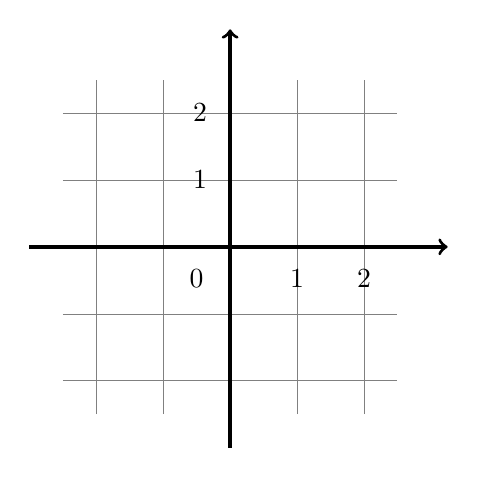
\begin{tikzpicture}[scale=0.85]
        \draw[help lines] (-2.5,-2.5) grid (2.5, 2.5);
        \draw[very thick, ->] (-3, 0) -- (3.25, 0);
        \draw[very thick, ->] (0, -3) -- (0, 3.25);
        \node[overlay, left] at (-0.2, 1) {$1$};
        \node[overlay, left] at (-0.2, 2) {$2$};
        \node[overlay, below] at (-0.5, -0.2) {$0$};
        \node[overlay, below] at (1, -0.2) {$1$};
        \node[overlay, below] at (2, -0.2) {$2$};
        \end{tikzpicture}
        \end{center}
\fi

\ifnum \Version=2
\question[2] Consider the autonomous differential equation $\displaystyle \frac{dy}{dt}= (y-k)(y+1-k^2)$.  Assume $k$ can be any real number. Draw the bifurcation diagram on the axes below. That is, plot the location of the critical points versus $k$. Please label your axes.
        \begin{center}
        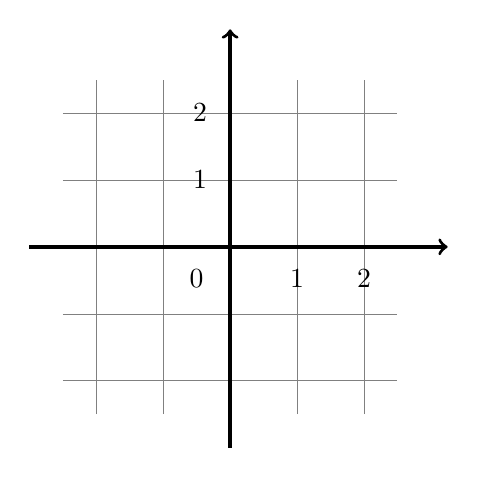
\begin{tikzpicture}[scale=0.85]
        \draw[help lines] (-2.5,-2.5) grid (2.5, 2.5);
        \draw[very thick, ->] (-3, 0) -- (3.25, 0);
        \draw[very thick, ->] (0, -3) -- (0, 3.25);
        \node[overlay, left] at (-0.2, 1) {$1$};
        \node[overlay, left] at (-0.2, 2) {$2$};
        \node[overlay, below] at (-0.5, -0.2) {$0$};
        \node[overlay, below] at (1, -0.2) {$1$};
        \node[overlay, below] at (2, -0.2) {$2$};
        \end{tikzpicture}
        \end{center}
\fi

\ifnum \Version=3
    \question[2] You do not need to show your work for this question. Consider the differential equation 
    \begin{align*}
        t^2y'' - 4ty' - 2y = 12
    \end{align*}
    The DE can be expressed in the form $\vec x\, ' = A\vec x + \vec g$, where 
    \begin{align*}
     A = \left( \hbox to 2cm{\vbox to 0.85cm{}} \right), \quad \vec g = \left( \hbox to 1.2cm{\vbox to 0.85cm{}} \right)
    \end{align*}
    Fill in the missing entries in the above to define $A$ and $\vec g$. 
\fi

\ifnum \Version=4
\question[2] Consider the autonomous differential equation $\displaystyle \frac{dy}{dt}= (y+k)(y^2-k)$.  Assume $k\ge0$. Draw the bifurcation diagram on the axes below. That is, plot the location of the critical points versus $k$. Please label your axes.
        \begin{center}
        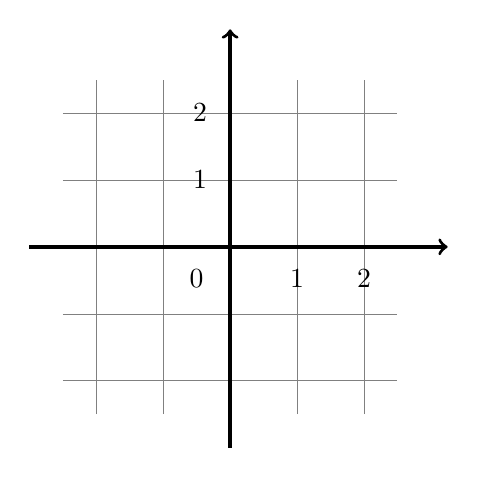
\begin{tikzpicture}[scale=0.85]
        \draw[help lines] (-2.5,-2.5) grid (2.5, 2.5);
        \draw[very thick, ->] (-3, 0) -- (3.25, 0);
        \draw[very thick, ->] (0, -3) -- (0, 3.25);
        \node[overlay, left] at (-0.2, 1) {$1$};
        \node[overlay, left] at (-0.2, 2) {$2$};
        \node[overlay, below] at (-0.5, -0.2) {$0$};
        \node[overlay, below] at (1, -0.2) {$1$};
        \node[overlay, below] at (2, -0.2) {$2$};
        \end{tikzpicture}
        \end{center}
\fi

\ifnum \Version=5
    \question[2] You do not need to show your work for this question. Consider the differential equation 
    \begin{align*}
        4y'' - t^2y' - 2ty = 12\cos(t)
    \end{align*}
    The DE can be expressed in the form $\vec x\, ' = A\vec x + \vec g$, where 
    \begin{align*}
     A = \left( \hbox to 2cm{\vbox to 0.85cm{}} \right), \quad \vec g = \left( \hbox to 1.2cm{\vbox to 0.85cm{}} \right)
    \end{align*}
    Fill in the missing entries in the above to define $A$ and $\vec g$. 
\fi




\ifnum \Version=6
\question[1] You do not need to show your work for this question. Consider the IVP below.
$$\displaystyle y' = \sqrt{4-t^2+y}, \ y(1) = 2$$   
Using the theorems we covered in lecture, fill in all of the appropriate circles below to indicate the intervals over which there must contain a unique solution to the IVP. 
\begin{itemize}
    \item[$\bigcirc$] $y \ge 4-t^2$
    \item[$\bigcirc$] $y \le 4-t^2$
    \item[$\bigcirc$] $y \le t^2-4$
    \item[$\bigcirc$] $y \ge t^2-4$
    \item[$\bigcirc$] none of the above
\end{itemize}
\ifnum \Solutions=1 {\color{DarkBlue} 
\textbf{Solutions:} the relevant theorem is below. 

    \begin{center}\begin{tikzpicture} \node [mybox](box){\begin{minipage}{0.95\textwidth} \vspace{4pt}

    If $f$ and $\frac{\partial f}{\partial y}$ are continuous over $\alpha < t < \beta$, and $\gamma < y < \delta$, which contains the point $(t_0,y_0)$, then there is a unique solution to the IVP $$y' = f(t,y), \quad y(t_0) = y_0$$ on an interval contained in $\alpha < t < \beta$. 
    
    \end{minipage}}; \node[fancytitle, rounded corners, thick, inner sep = 4pt, right=10pt] at (box.north west) {Theorem 2.4.2: Existence and Uniqueness of 1st Order Nonlinear IVP};
    \end{tikzpicture}\end{center}
    
    Taking the partial derivative with respect to $y$:
\begin{align}
    \frac{\partial f}{\partial y} &= \frac{1}{\sqrt{4-t^2+y}}\\
\end{align}
The relevant functions are 
\begin{align}
    f(t,y) &= \sqrt{4-t^2+y} \\
    \frac{\partial f}{\partial y} &= \frac{1}{\sqrt{4-t^2+y}}
\end{align}
They are real and continuous over $$4-t^2+y > 0$$ and this interval also contains $t_0 = 0$ and $y(t_0)$. So the interval over which there must contain a unique solution is $$y > t^2-4$$ 
} 
\else 
\fi
\fi 




\ifnum \Version=7
\question[1] You do not need to show your work for this question. Consider the IVP below.
$$\displaystyle (t+3)y' + \sqrt{4-t^2}\,y = t^4, \ y(1) = 9$$   
Using the theorems we covered in lecture, fill in all of the appropriate circles below to indicate the intervals over which there must contain a unique solution to the IVP. 
\begin{itemize}
    \item[$\bigcirc$] $-3 < t \le 2$
    \item[$\bigcirc$] $-2 \le t \le 2$
    \item[$\bigcirc$] $-2 \le t \le 3$    
    \item[$\bigcirc$] $-\infty \le t < -3$
    \item[$\bigcirc$] none of the above
\end{itemize}
\ifnum \Solutions=1 {\color{DarkBlue} 
\textbf{Solutions:} convert to standard form:
\begin{align}
    y' + \frac{\sqrt{4-t^2}}{t+3}\,y = \frac{t^4}{t+3}
\end{align}
The coefficients are real and continuous over $$-2\le t \le 2$$ and this interval also contains $t_0 = 1$. So the interval over which there must contain a unique solution is $-2\le t \le 2$. 
} 
\else 
\fi
\fi 



\ifnum \Version=8
\question[1] You do not need to show your work for this question. Consider the IVP below.
$$\displaystyle y' = \sqrt{4-t^2-y}, \ y(0) = 2$$   
Using the theorems we covered in lecture, fill in all of the appropriate circles below to indicate the intervals over which there must contain a unique solution to the IVP. 
\begin{itemize}
    \item[$\bigcirc$] $y \ge 4-t^2$
    \item[$\bigcirc$] $y \le 4-t^2$
    \item[$\bigcirc$] $y \le t^2-4$
    \item[$\bigcirc$] $y \ge t^2-4$
    \item[$\bigcirc$] none of the above
\end{itemize}
\ifnum \Solutions=1 {\color{DarkBlue} 
\textbf{Solutions:} partial derivative with respect to $y$:
\begin{align}
    \frac{\partial f}{\partial y} &= \frac{-1}{\sqrt{4-t^2-y}}
\end{align}
The coefficients are real and continuous over $$4-t^2-y\ge 0$$ and this interval also contains $t_0 = 0$ and $y(t_0)$. So the interval over which there must contain a unique solution is $y \le 4-t^2$. 
} 
\else 
\fi
\fi 



\ifnum \Version=9
\question[1] You do not need to show your work for this question. Consider the IVP below.
$$\displaystyle y' = \sqrt{4-t^2+y}, \ y(0) = 2$$   
Using the theorems we covered in lecture, fill in all of the appropriate circles below to indicate the intervals over which there must contain a unique solution to the IVP. 
\begin{itemize}
    \item[$\bigcirc$] $y \ge 4-t^2$
    \item[$\bigcirc$] $y \le 4-t^2$
    \item[$\bigcirc$] $y \le t^2-4$
    \item[$\bigcirc$] $y \ge t^2-4$
    \item[$\bigcirc$] none of the above
\end{itemize}
\ifnum \Solutions=1 {\color{DarkBlue} 
\textbf{Solutions:} partial derivative with respect to $y$:
\begin{align}
    \frac{\partial f}{\partial y} &= \frac{1}{\sqrt{4-t^2+y}}\\
\end{align}
The coefficients are real and continuous over $$4-t^2+y\ge 0$$ and this interval also contains $t_0 = 0$ and $y(t_0)$. So the interval over which there must contain a unique solution is $y \ge t^2-4$. 
} 
\else 
\fi
\fi 




    \ifnum \Version=6
\question[3] Consider the system $$\vec x \, ' = A\vec x, \quad A = \begin{pmatrix} -3&-4\\1&-1 \end{pmatrix}, \quad \vec x = \begin{pmatrix} x(t)\\y(t)\end{pmatrix} $$ The eigenvalues of $A$ are $\lambda = -2\pm i\sqrt 3$. Sketch the phase portrait of the system. Sketch at least two solution curves. Please indicate the direction of motion on your solution curves. Don't forget to label your axes.   

\ifnum \Solutions=1 {\color{DarkBlue} 
\textbf{Solutions:} solution curves should \textbf{spiral towards} the origin and rotate \textbf{counter clockwise}. Axes should be labelled. Ok to only draw only two solution curves. 
    \begin{center}
    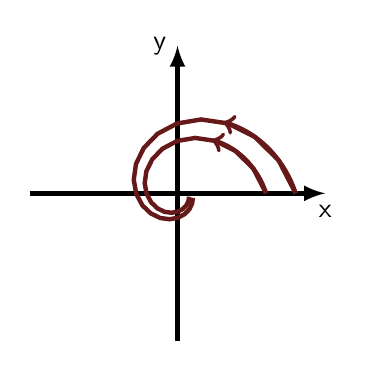
\begin{tikzpicture}[scale=0.75]
      \draw[ultra thick,->,>=latex] (-2.5,0)--(2.5,0) node[below] {x};
      \draw[ultra thick,->,>=latex] (0,-2.5)--(0,2.5) node[left] {y};      
      \draw[domain=0:6,ultra thick,samples=20,DarkRed] plot ({cos(deg(\x))*2*exp(-\x/3},{sin(deg(\x))*2*exp(-\x/3});
      \draw[domain=0:1,->,ultra thick,samples=20,DarkRed] plot ({cos(deg(\x))*2*exp(-\x/3},{sin(deg(\x))*2*exp(-\x/3});
      \draw[domain=0:6,ultra thick,samples=20,DarkRed] plot ({.75*cos(deg(\x))*2*exp(-\x/3},{.75*sin(deg(\x))*2*exp(-\x/3});
      \draw[domain=0:1,->,ultra thick,samples=20,DarkRed] plot ({.75*cos(deg(\x))*2*exp(-\x/3},{.75*sin(deg(\x))*2*exp(-\x/3});
    \end{tikzpicture}
    \end{center} 
} 
\else 
    \begin{center}
    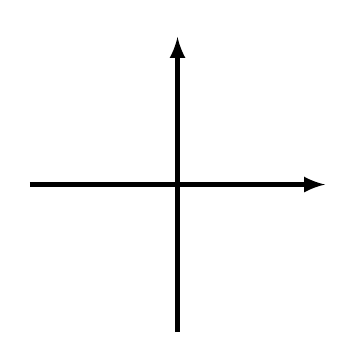
\begin{tikzpicture}[scale=0.75]
      \draw[ultra thick,->,>=latex] (-2.5,0)--(2.5,0) node[below] {};
      \draw[ultra thick,->,>=latex] (0,-2.5)--(0,2.5) node[left] {};         
    \end{tikzpicture}
    \end{center} 
\fi
\fi


\ifnum \Version=7
\question[3] Consider the system $$\vec x \, ' = A\vec x, \quad A = \begin{pmatrix} 3&2\\-5&1 \end{pmatrix}, \quad \vec x = \begin{pmatrix} x(t)\\y(t)\end{pmatrix} $$ The eigenvalues of $A$ are $\lambda = 2\pm  3i$. Sketch the phase portrait of the system. Sketch at least two solution curves. Please indicate the direction of motion on your solution curves. Don't forget to label your axes.   

\ifnum \Solutions=1 {\color{DarkBlue} 
\textbf{Solutions:} solution curves should \textbf{spiral away} from the origin and rotate \textbf{clockwise}. Axes should be labelled. Ok to only draw only two solution curves. 
\begin{center}
    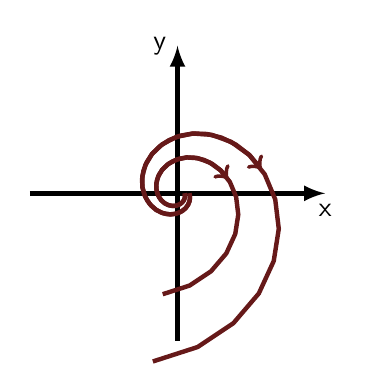
\begin{tikzpicture}[scale=0.75]
      \draw[ultra thick,->,>=latex] (-2.5,0)--(2.5,0) node[below] {x};
      \draw[ultra thick,->,>=latex] (0,-2.5)--(0,2.5) node[left] {y};      
      \draw[domain=0:8,ultra thick,samples=30,DarkRed] plot ({cos(deg(\x))*0.12*exp(\x/3)},{-sin(deg(\x))*0.12*exp(\x/3)});
      \draw[domain=0:6,->,ultra thick,samples=30,DarkRed] plot ({cos(deg(\x))*0.12*exp(\x/3)},{-sin(deg(\x))*0.12*exp(\x/3)});
      \draw[domain=0:8,ultra thick,samples=30,DarkRed] plot ({cos(deg(\x))*0.2*exp(\x/3)},{-sin(deg(\x))*0.2*exp(\x/3)});
      \draw[domain=0:6,->,ultra thick,samples=30,DarkRed] plot ({cos(deg(\x))*0.2*exp(\x/3)},{-sin(deg(\x))*0.2*exp(\x/3)});      
    \end{tikzpicture}
\end{center} 
} 
\else 
\begin{center}
    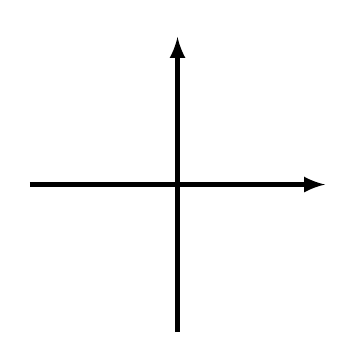
\begin{tikzpicture}[scale=0.75]
      \draw[ultra thick,->,>=latex] (-2.5,0)--(2.5,0) node[below] {};
      \draw[ultra thick,->,>=latex] (0,-2.5)--(0,2.5) node[left] {};         
    \end{tikzpicture}
\end{center} 
\fi
\fi






\ifnum \Version=8
\question[3] Consider the system $$\vec x \, ' = A\vec x, \quad A = \begin{pmatrix} -3&-4\\1&-1 \end{pmatrix}, \quad \vec x = \begin{pmatrix} x(t)\\y(t)\end{pmatrix} $$ The eigenvalues of $A$ are $\lambda = -2\pm i\sqrt 3$. Sketch the phase portrait of the system. Sketch at least two solution curves. Please indicate the direction of motion on your solution curves. Don't forget to label your axes.   

\ifnum \Solutions=1 {\color{DarkBlue} 
\textbf{Solutions:} solution curves should spiral towards center and rotate counter clockwise. Axes should be labelled. Ok to only draw only two solution curves. 
    \begin{center}
    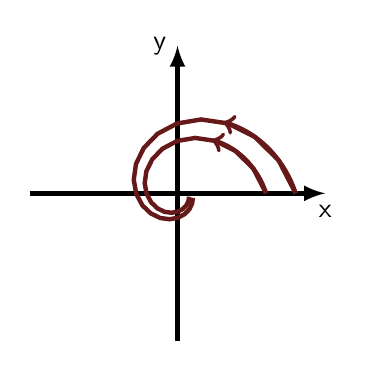
\begin{tikzpicture}[scale=0.75]
      \draw[ultra thick,->,>=latex] (-2.5,0)--(2.5,0) node[below] {x};
      \draw[ultra thick,->,>=latex] (0,-2.5)--(0,2.5) node[left] {y};      
      \draw[domain=0:6,ultra thick,samples=20,DarkRed] plot ({cos(deg(\x))*2*exp(-\x/3},{sin(deg(\x))*2*exp(-\x/3});
      \draw[domain=0:1,->,ultra thick,samples=20,DarkRed] plot ({cos(deg(\x))*2*exp(-\x/3},{sin(deg(\x))*2*exp(-\x/3});
      \draw[domain=0:6,ultra thick,samples=20,DarkRed] plot ({.75*cos(deg(\x))*2*exp(-\x/3},{.75*sin(deg(\x))*2*exp(-\x/3});
      \draw[domain=0:1,->,ultra thick,samples=20,DarkRed] plot ({.75*cos(deg(\x))*2*exp(-\x/3},{.75*sin(deg(\x))*2*exp(-\x/3});
    \end{tikzpicture}
    \end{center} 
} 
\else 
    \begin{center}
    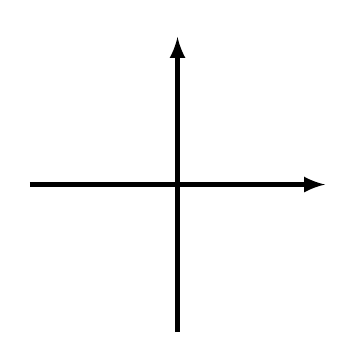
\begin{tikzpicture}[scale=0.75]
      \draw[ultra thick,->,>=latex] (-2.5,0)--(2.5,0) node[below] {};
      \draw[ultra thick,->,>=latex] (0,-2.5)--(0,2.5) node[left] {};         
    \end{tikzpicture}
    \end{center} 
\fi
\fi




\ifnum \Version=9
\question[3] Consider the system $$\vec x \, ' = A\vec x, \quad A = \begin{pmatrix} 1&-4\\1&3 \end{pmatrix}, \quad \vec x = \begin{pmatrix} x(t)\\y(t)\end{pmatrix} $$ The eigenvalues of $A$ are $\lambda = 2\pm i\sqrt 3$. Sketch the phase portrait of the system. Sketch at least two solution curves. Please indicate the direction of motion on your solution curves. Don't forget to label your axes.   

\ifnum \Solutions=1 {\color{DarkBlue} 
\textbf{Solutions:} solution curves should spiral away from the origin and rotate counter clockwise. Axes should be labelled. Ok to only draw only two solution curves. 
    \begin{center}
    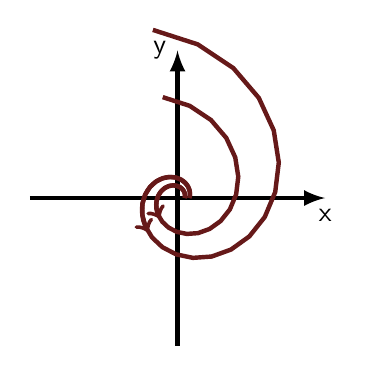
\begin{tikzpicture}[scale=0.75]
      \draw[ultra thick,->,>=latex] (-2.5,0)--(2.5,0) node[below] {x};
      \draw[ultra thick,->,>=latex] (0,-2.5)--(0,2.5) node[left] {y};      
      \draw[domain=0:8,ultra thick,samples=30,DarkRed] plot ({cos(deg(\x))*0.12*exp(\x/3)},{sin(deg(\x))*0.12*exp(\x/3)});
      \draw[domain=0:4,->,ultra thick,samples=30,DarkRed] plot ({cos(deg(\x))*0.12*exp(\x/3)},{sin(deg(\x))*0.12*exp(\x/3)});
      \draw[domain=0:8,ultra thick,samples=30,DarkRed] plot ({cos(deg(\x))*0.2*exp(\x/3)},{sin(deg(\x))*0.2*exp(\x/3)});
      \draw[domain=0:4,->,ultra thick,samples=30,DarkRed] plot ({cos(deg(\x))*0.2*exp(\x/3)},{sin(deg(\x))*0.2*exp(\x/3)});      
    \end{tikzpicture}
    \end{center} 
} 
\else 
    \begin{center}
    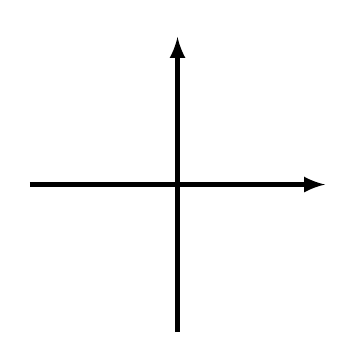
\begin{tikzpicture}[scale=0.75]
      \draw[ultra thick,->,>=latex] (-2.5,0)--(2.5,0) node[below] {};
      \draw[ultra thick,->,>=latex] (0,-2.5)--(0,2.5) node[left] {};         
    \end{tikzpicture}
    \end{center} 
\fi
\fi



    
\ifnum \Version>5
\question[3] A tank originally contains 50 L of water with 6 kg of salt. Water containing $\frac{1}{20}$ kg of salt per litre is entering at a rate of 4 L/hour, and the well-stirred solution in the tank is leaving at 1 L/hour. 

\begin{parts}
    \part Write down an IVP for $V(t)$, which is the amount of fluid in the tank at time $t$. You do not need to solve your IVP. 
    
    \ifnum \Solutions=1 {\color{DarkBlue} 
        The volume of fluid in the tank is
        $$V = 50 + 3t$$
        By differentiating, the IVP for $V(t)$ is
        $$\frac{dV}{dt} = 3, \quad V(0) = 50$$
        }
    \else
    \vspace{6cm}
    \fi
    
    \part Write down an IVP for $Q(t)$, for the amount of salt in the tank. You do not need to solve the IVP. 
    
    \ifnum \Solutions=1 {\color{DarkBlue} 
        The DE is
        \begin{align}
            \frac{dQ}{dt} &= \left( \text{rate salt coming in} \right) - \left( \text{rate of salt going out} \right) \\
            \frac{dQ}{dt} &= 4\cdot \frac{1}{20} - \frac{Q}{V}
        \end{align}
        The IVP is
        \begin{align}
            \frac{dQ}{dt} &= \frac{1}{5} - \frac{Q}{50+3t}, \quad Q(0) = 6
        \end{align}        
        }
        \fi
    \fi
    
\end{parts}


        

    \newpage        
    \newpage 
\ifnum \Version=1  
\question[4] Solve the initial value problem and solve for $y$ to obtain an explicit expression for $y$ in terms of $t$. Please show your work.
$$\displaystyle t\,\frac{dy}{dt} = \frac{\cos(t)}{t^2} - 3y, \quad y(\pi) = 2, \quad t > 0$$.
\fi

\ifnum \Version=2
\question[4] Solve the initial value problem and solve for $y$ to obtain an explicit expression for $y$ in terms of $t$. Please show your work.
$$\displaystyle \frac{dy}{dt} = 12e^{3t}e^{-2y}, \quad y(0) = 2, \quad t \ge 0$$.
\fi

\ifnum \Version=3
\question[4] Solve the initial value problem and solve for $y$ to obtain an explicit expression for $y$ in terms of $t$. Please show your work.
$$\displaystyle t\,\frac{dy}{dt} + 3y =  36 t^{-2}e^{-t}, \ y(1) = 0, \quad t > 0$$.
\fi   

\ifnum \Version=4
\question[4] Solve the initial value problem and solve for $y$ to obtain an expression for $y$ in terms of $t$. Please show your work.
$$\displaystyle \frac{dy}{dt} = \frac{16e^{2t}}{y}, \quad y(1) = 2, \quad t > 0$$.
\fi

\ifnum \Version=5
\question[4] Solve the initial value problem and solve for $y$ to obtain an explicit expression for $y$ in terms of $t$. Please show your work.
$$\displaystyle t\,\frac{dy}{dt} + 2y =  36 t^{-1}e^{t}, \ y(1) = 2e, \quad t > 0$$.
\fi   



\ifnum \Version=6
\question[4] 
Solve the initial value problem and solve for $y$ to obtain an explicit expression for $y$ in terms of $t$. Please show your work.
$$\displaystyle t\,\frac{dy}{dt} + 4y =  24 t^{-3}e^{2t}, \ y(1) = 2, \quad t > 0$$.

\ifnum \Solutions=1 {\color{DarkBlue} 
\textbf{Solutions:}
To solve the differential equation \( t y' + 4 y = 24 t^{-3} e^{2t} \) with the initial condition \( y(1) = 2 \), we can follow these steps.
\begin{enumerate}
    \item Rewrite the DE in standard form:
   \[ y' + \frac{4}{t} y = 24 t^{-4} e^{2t} \]
   \item Integrating factor:
   \[ \mu(t) = e^{\int \frac{4}{t} \, dt} = e^{4 \ln |t|} = t^4 \]
   \item Multiply both sides of the differential equation by the integrating factor:
   \begin{align*}
       t^4 y' + 4 t^3 y &= 24 e^{2t} \\
       \frac{d}{dt} (t^4 y) &= 24 e^{2t}
   \end{align*} 
   \item Integrate both sides with respect to \( t \) and solve for $y$:
   \begin{align}
       t^4 y &= \int 24 e^{2t} \, dt + C \\
       t^4 y &= 12 e^{2t} + C \\
        y &= \frac{12 e^{2t} + C}{t^4} 
   \end{align} 
   \item Apply the initial condition \( y(1) = 2 \):
   \[ 2 = \frac{12 e^{2 \cdot 1} + C}{1^4} \]
   \[ 2 = 12 e^2 + C \]
   \[ C = 2 - 12 e^2 \]
   \item Substitute \( C \) back into the solution:
   \[ y = \frac{12 e^{2t} + 2 - 12 e^2}{t^4} \]
\end{enumerate}
} 
\else 
\newpage
\fi
\fi   





\ifnum \Version=7
\question[4] 
Solve the initial value problem and solve for $y$ to obtain an explicit expression for $y$ in terms of $t$. Please show your work.
$$\displaystyle t\,\frac{dy}{dt} + 5y =  20 t^{-4}e^{2t}, \ y(1) = e^2, \quad t > 0$$.

\ifnum \Solutions=1 {\color{DarkBlue} 
\textbf{Solutions:}
To solve the differential equation \( t y' + 5 y = 20 t^{-3} e^{2t} \) with the initial condition \( y(1) = 2 \), we can follow these steps.
\begin{enumerate}
    \item Rewrite the DE in standard form:
   \[ y' + \frac{5}{t} y = 20 t^{-4} e^{2t} \]
   \item Integrating factor:
   \[ \mu(t) = e^{\int \frac{5}{t} \, dt} = e^{5 \ln |t|} = t^5 \]
   \item Multiply both sides of the differential equation by the integrating factor:
   \begin{align*}
       t^5 y' + 5 t^4 y &= 20 e^{2t} \\
       \frac{d}{dt} (t^5 y) &= 20 e^{2t}
   \end{align*} 
   \item Integrate both sides with respect to \( t \) and solve for $y$:
   \begin{align}
       t^5 y &= \int 20 e^{2t} \, dt + C \\
       t^5 y &= 10 e^{2t} + C \\
        y &= \frac{10 e^{2t} + C}{t^5} 
   \end{align} 
   \item Apply the initial condition \( y(1) = e^2 \):
   \[ e^2 = \frac{10 e^{2 \cdot 1} + C}{1^5} \]
   \[ e^2 = 10 e^2 + C \]
   \[ C = - 9 e^2 \]
   \item Substitute \( C \) back into the solution:
   \[ y = \frac{10 e^{2t} - 9 e^2}{t^5} \]
\end{enumerate}
} 
\else 
\newpage
\fi
\fi   






\ifnum \Version=8
\question[4] 
Solve the initial value problem and solve for $y$ to obtain an explicit expression for $y$ in terms of $t$. Please show your work.
$$\displaystyle t\,\frac{dy}{dt} + 6y =  24 t^{-5}e^{4t}, \ y(1) = 8e^4, \quad t > 0$$.

\ifnum \Solutions=1 {\color{DarkBlue} 
\textbf{Solutions:}
To solve the DE with the given initial condition we can follow these steps.
\begin{enumerate}
    \item Rewrite the DE in standard form:
   \[ y' + \frac{6}{t} y = 24 t^{-6} e^{4t} \]
   \item Integrating factor:
   \[ \mu(t) = e^{\int \frac{6}{t} \, dt} = e^{6 \ln |t|} = t^6 \]
   \item Multiply both sides of the differential equation by the integrating factor:
   \begin{align*}
       t^6 y' + 6 t^5 y &= 24 e^{4t} \\
       \frac{d}{dt} (t^6 y) &= 24 e^{4t}
   \end{align*} 
   \item Integrate both sides with respect to \( t \) and solve for $y$:
   \begin{align}
       t^6 y &= \int 24 e^{4t} \, dt + C \\
       t^6 y &= 6 e^{4t} + C \\
        y &= \frac{6 e^{4t} + C}{t^6} 
   \end{align} 
   \item Apply the initial condition:
   \[ 8e^4 = \frac{6 e^{4 \cdot 1} + C}{1^5} \]
   \[ 8e^4 = 6 e^4 + C \]
   \[ C = 2 e^4 \]
   \item Substitute \( C \) back into the solution:
   \[ y = \frac{6 e^{4t} +2 e^4}{t^6} \]
\end{enumerate}
} 
\else 
\newpage
\fi
\fi   



\ifnum \Version=9
\question[4] 
Solve the initial value problem and solve for $y$ to obtain an explicit expression for $y$ in terms of $t$. Please show your work.
$$\displaystyle t\,\frac{dy}{dt} + 5y =  20 t^{-4}e^{2t}, \ y(1) = e^2, \quad t > 0$$.

\ifnum \Solutions=1 {\color{DarkBlue} 
\textbf{Solutions:}
To solve the differential equation \( t y' + 5 y = 20 t^{-3} e^{2t} \) with the initial condition \( y(1) = 2 \), we can follow these steps.
\begin{enumerate}
    \item Rewrite the DE in standard form:
   \[ y' + \frac{5}{t} y = 20 t^{-4} e^{2t} \]
   \item Integrating factor:
   \[ \mu(t) = e^{\int \frac{5}{t} \, dt} = e^{5 \ln |t|} = t^5 \]
   \item Multiply both sides of the differential equation by the integrating factor:
   \begin{align*}
       t^5 y' + 5 t^4 y &= 20 e^{2t} \\
       \frac{d}{dt} (t^5 y) &= 20 e^{2t}
   \end{align*} 
   \item Integrate both sides with respect to \( t \) and solve for $y$:
   \begin{align}
       t^5 y &= \int 20 e^{2t} \, dt + C \\
       t^5 y &= 10 e^{2t} + C \\
        y &= \frac{10 e^{2t} + C}{t^5} 
   \end{align} 
   \item Apply the initial condition \( y(1) = e^2 \):
   \[ e^2 = \frac{10 e^{2 \cdot 1} + C}{1^5} \]
   \[ e^2 = 10 e^2 + C \]
   \[ C = - 9 e^2 \]
   \item Substitute \( C \) back into the solution:
   \[ y = \frac{10 e^{2t} - 9 e^2}{t^5} \]
\end{enumerate}
} 
\else 
\newpage
\fi
\fi   
        
    \newpage 

\ifnum \Version=1  
\question[7] Consider the system $$\vec x \, ' = A\vec x, \quad A = \begin{pmatrix} 0&3\\5&2 \end{pmatrix}, \quad \vec x = \begin{pmatrix} x(t)\\y(t)\end{pmatrix} $$.
\begin{parts}
    \part Determine the eigenvalues of $A$. Please show your work. \vspace{5cm}
    \part Determine the eigenvectors of $A$. Please show your work. \vspace{7cm}
    \part Sketch the phase portrait of the system on the axes below. Please indicate the direction of motion on your solution curves and draw the eigenspaces corresponding to real eigenvalues (if any). Please also label your axes. 
    \begin{center}
    \begin{tikzpicture}[scale=0.85]
    \draw[very thick, ->] (-3, 0) -- (3.25, 0);
    \draw[very thick, ->] (0, -3) -- (0, 3.25);
    \end{tikzpicture}
    \end{center}
\end{parts}
\fi

\ifnum \Version=2
\question[7] Consider the system $$\vec x \, ' = A\vec x, \quad A = \begin{pmatrix} 4&3\\3&-4 \end{pmatrix}, \quad \vec x = \begin{pmatrix} x(t)\\y(t)\end{pmatrix} $$.
\begin{parts}
    \part Determine the eigenvalues of $A$. Please show your work. \vspace{5cm}
    \part Determine the eigenvectors of $A$. Please show your work. \vspace{7cm}
    \part Sketch the phase portrait of the system on the axes below. Please indicate the direction of motion on your solution curves and draw the eigenspaces corresponding to real eigenvalues (if any). Please also label your axes. 
    \begin{center}
    \begin{tikzpicture}[scale=0.85]
    \draw[very thick, ->] (-3, 0) -- (3.25, 0);
    \draw[very thick, ->] (0, -3) -- (0, 3.25);
    \end{tikzpicture}
    \end{center}
\end{parts}
\fi

\ifnum \Version=3
\question[7] Consider the system $$\vec x \, ' = A\vec x, \quad A = \begin{pmatrix} 5&4\\-3&-3 \end{pmatrix}, \quad \vec x = \begin{pmatrix} x(t)\\y(t)\end{pmatrix} $$.
\begin{parts}
    \part Determine the eigenvalues of $A$. Please show your work. \vspace{5cm}
    \part Determine the eigenvectors of $A$. Please show your work. \vspace{7cm}
    \part Sketch the phase portrait of the system on the axes below. Please indicate the direction of motion on your solution curves and draw the eigenspaces corresponding to real eigenvalues (if any). Please also label your axes. 
    \begin{center}
    \begin{tikzpicture}[scale=0.85]
    \draw[very thick, ->] (-3, 0) -- (3.25, 0);
    \draw[very thick, ->] (0, -3) -- (0, 3.25);
    \end{tikzpicture}
    \end{center}
\end{parts}
\fi

\ifnum \Version=4
\question[7] Consider the system $$\vec x \, ' = A\vec x, \quad A = \begin{pmatrix} 3&4\\-3&-5 \end{pmatrix}, \quad \vec x = \begin{pmatrix} x(t)\\y(t)\end{pmatrix} $$.
\begin{parts}
    \part Determine the eigenvalues of $A$. Please show your work. \vspace{5cm}
    \part Determine the eigenvectors of $A$. Please show your work. \vspace{7cm}
    \part Sketch the phase portrait of the system on the axes below. Please indicate the direction of motion on your solution curves and draw the eigenspaces corresponding to real eigenvalues (if any). Please also label your axes. 
    \begin{center}
    \begin{tikzpicture}[scale=0.85]
    \draw[very thick, ->] (-3, 0) -- (3.25, 0);
    \draw[very thick, ->] (0, -3) -- (0, 3.25);
    \end{tikzpicture}
    \end{center}
\end{parts}
\fi

\ifnum \Version=5
\question[7] Consider the system $$\vec x \, ' = A\vec x, \quad A = \begin{pmatrix} 4&4\\-3&-4 \end{pmatrix}, \quad \vec x = \begin{pmatrix} x(t)\\y(t)\end{pmatrix} $$.
\begin{parts}
    \part Determine the eigenvalues of $A$. Please show your work. \vspace{5cm}
    \part Determine the eigenvectors of $A$. Please show your work. \vspace{7cm}
    \part Sketch the phase portrait of the system on the axes below. Please indicate the direction of motion on your solution curves and draw the eigenspaces corresponding to real eigenvalues (if any). Please also label your axes. 
    \begin{center}
    \begin{tikzpicture}[scale=0.85]
    \draw[very thick, ->] (-3, 0) -- (3.25, 0);
    \draw[very thick, ->] (0, -3) -- (0, 3.25);
    \end{tikzpicture}
    \end{center}
\end{parts}
\fi



\ifnum \Version=6
    \question[6] Consider the IVP $$\vec x \, ' = A\vec x, \quad A = \begin{pmatrix} -1&3\\3&-1 \end{pmatrix}, \quad \vec x = \begin{pmatrix} x(t)\\y(t)\end{pmatrix}, \quad \vec x(0) = \begin{pmatrix} 2\\2 \end{pmatrix}$$ The eigenvalues of $A$ are $\lambda_1 = -4$ and $\lambda_2 = 2$. 
    \begin{parts}
        \part Determine the eigenvectors of $A$. Please show your work. 
        
        \ifnum \Solutions=1 {\color{DarkBlue} 
        \textbf{Solutions:}
        For $\lambda_1$:
        \begin{align}
            A - \lambda_1 I = \begin{pmatrix} 3&3\\3&3\end{pmatrix} \ \Rightarrow \ v_1 = \begin{pmatrix} -1\\1 \end{pmatrix}
        \end{align}
        For $\lambda_2$:
        \begin{align}
            A - \lambda_2 I = \begin{pmatrix} -3&3\\3&-3\end{pmatrix} \ \Rightarrow \ v_2 = \begin{pmatrix} 1\\1 \end{pmatrix}
        \end{align}    
        } 
        \else 
            \vspace{6cm}   
        \fi        
        \part Use the given eigenvalues and the eigenvectors that you calculated in part (a) to solve the IVP.  
        
        \ifnum \Solutions=1 {\color{DarkBlue} 
        \textbf{Solutions:} the general solution to the DE is:
        $$\vec x = c_1 e^{-4t}\begin{pmatrix} -1\\1\end{pmatrix} + c_2e^{2t} \begin{pmatrix} 1\\1\end{pmatrix}$$
        Use initial condition:
        \begin{align}
            \begin{pmatrix} 2\\2\end{pmatrix} &= c_1\begin{pmatrix}-1\\1 \end{pmatrix}+ c_2 \begin{pmatrix} 1\\1\end{pmatrix} \ \Rightarrow \ c_1 = 0, c_2 = 2 \ \Rightarrow \ 
            \vec x (t) = 2e^{2t} \begin{pmatrix} 1\\1\end{pmatrix}
        \end{align}
        } 
        \else 
        \vspace{7cm}
    \fi
    \part Sketch the phase portrait of the system on the axes below. Please indicate the direction of motion on your solution curves and draw the eigenspaces corresponding to real eigenvalues (if any). Please also label your axes. 
    
    \ifnum \Solutions=1 {\color{DarkBlue} 
    \textbf{Solutions:}
        \begin{center}
        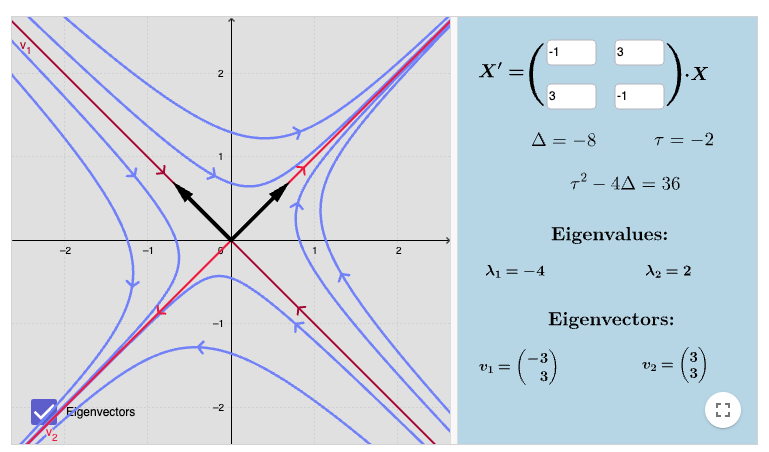
\includegraphics[width=5in]{Images/ImgPhasePlane1331.png}
        \end{center}         
    } 
    \else 
        \begin{center}
        \begin{tikzpicture}[scale=0.85]
        \draw[very thick, ->] (-3, 0) -- (3.25, 0);
        \draw[very thick, ->] (0, -3) -- (0, 3.25);
        \end{tikzpicture}
        \end{center}    
    \fi    

\end{parts}
\fi





\ifnum \Version=7
    \question[6] Consider the IVP $$\vec x \, ' = A\vec x, \quad A = \begin{pmatrix} 0&3\\3&8 \end{pmatrix}, \quad \vec x = \begin{pmatrix} x(t)\\y(t)\end{pmatrix}, \quad \vec x(0) = \begin{pmatrix} -3\\1 \end{pmatrix}$$ The eigenvalues of $A$ are $\lambda_1 = -1$ and $\lambda_2 = 9$. 
    \begin{parts}
        \part Determine the eigenvectors of $A$. Please show your work. 
        
        \ifnum \Solutions=1 {\color{DarkBlue} 
        \textbf{Solutions:}
        For $\lambda_1$:
        \begin{align}
            A - \lambda_1 I = \begin{pmatrix} 1&3\\3&9\end{pmatrix} \ \Rightarrow \ v_1 = \begin{pmatrix} -3\\1 \end{pmatrix}
        \end{align}
        For $\lambda_2$:
        \begin{align}
            A - \lambda_2 I = \begin{pmatrix} -9&3\\3&-1\end{pmatrix} \ \Rightarrow \ v_2 = \begin{pmatrix} 1\\3 \end{pmatrix}
        \end{align}    
        } 
        \else 
            \vspace{6cm}   
        \fi        
        \part Use the given eigenvalues and the eigenvectors that you calculated in part (a) to solve the IVP.  
        
        \ifnum \Solutions=1 {\color{DarkBlue} 
        \textbf{Solutions:} the general solution to the DE is:
        $$\vec x = c_1 e^{-t}\begin{pmatrix} -3\\1\end{pmatrix} + c_2e^{9t} \begin{pmatrix} 1\\3\end{pmatrix}$$
        Use initial condition:
        \begin{align}
            \begin{pmatrix} -3\\1\end{pmatrix} &= c_1\begin{pmatrix}-3\\1 \end{pmatrix}+ c_2 \begin{pmatrix} 1\\3\end{pmatrix} \ \Rightarrow \ c_1 = 1, c_2 = 0 \ \Rightarrow \ 
            \vec x (t) = e^{-t} \begin{pmatrix} -3\\1\end{pmatrix}
        \end{align}
        } 
        \else 
        \vspace{7cm}
    \fi
    \part Sketch the phase portrait of the system on the axes below. Please indicate the direction of motion on your solution curves and draw the eigenspaces corresponding to real eigenvalues (if any). Please also label your axes. 
    
    \ifnum \Solutions=1 {\color{DarkBlue} 
    \textbf{Solutions:}
        \begin{center}
        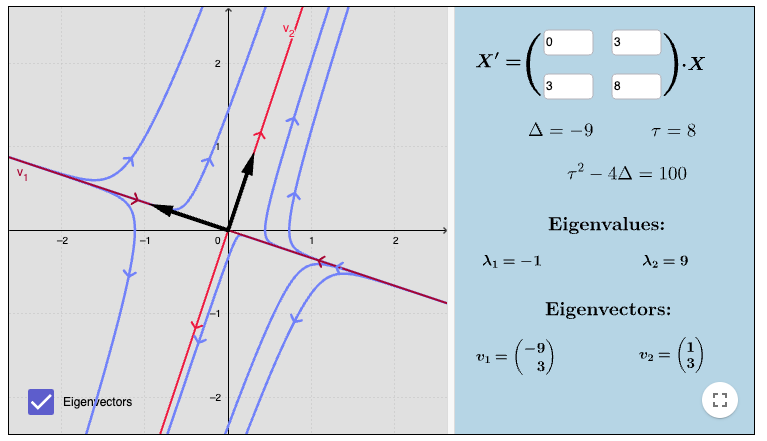
\includegraphics[width=5in]{Images/ImgPhasePlane0338.png}
        \end{center}         
    } 
    \else 
        \begin{center}
        \begin{tikzpicture}[scale=0.85]
        \draw[very thick, ->] (-3, 0) -- (3.25, 0);
        \draw[very thick, ->] (0, -3) -- (0, 3.25);
        \end{tikzpicture}
        \end{center}    
    \fi    

\end{parts}
\fi








\ifnum \Version=8
    \question[6] Consider the IVP $$\vec x \, ' = A\vec x, \quad A = \begin{pmatrix} -1&3\\3&7 \end{pmatrix}, \quad \vec x = \begin{pmatrix} x(t)\\y(t)\end{pmatrix}, \quad \vec x(0) = \begin{pmatrix} 1\\3 \end{pmatrix}$$ The eigenvalues of $A$ are $\lambda_1 = -2$ and $\lambda_2 = 8$. 
    \begin{parts}
        \part Determine the eigenvectors of $A$. Please show your work. 
        
        \ifnum \Solutions=1 {\color{DarkBlue} 
        \textbf{Solutions:}
        For $\lambda_1$:
        \begin{align}
            A - \lambda_1 I = \begin{pmatrix} 1&3\\3&9\end{pmatrix} \ \Rightarrow \ v_1 = \begin{pmatrix} -3\\1 \end{pmatrix}
        \end{align}
        For $\lambda_2$:
        \begin{align}
            A - \lambda_2 I = \begin{pmatrix} -9&3\\3&-1\end{pmatrix} \ \Rightarrow \ v_2 = \begin{pmatrix} 1\\3 \end{pmatrix}
        \end{align}    
        } 
        \else 
            \vspace{6cm}   
        \fi        
        \part Use the given eigenvalues and the eigenvectors that you calculated in part (a) to solve the IVP.  
        
        \ifnum \Solutions=1 {\color{DarkBlue} 
        \textbf{Solutions:} the general solution to the DE is:
        $$\vec x = c_1 e^{-4t}\begin{pmatrix} -1\\1\end{pmatrix} + c_2e^{2t} \begin{pmatrix} 1\\1\end{pmatrix}$$
        Use initial condition:
        \begin{align}
            \begin{pmatrix} 1\\3\end{pmatrix} &= c_1\begin{pmatrix}-3\\1 \end{pmatrix}+ c_2 \begin{pmatrix} 1\\3\end{pmatrix} \ \Rightarrow \ c_1 = 0, c_2 = 1 \ \Rightarrow \ 
            \vec x (t) = e^{8t} \begin{pmatrix} 1\\3\end{pmatrix}
        \end{align}
        } 
        \else 
        \vspace{7cm}
    \fi
    \part Sketch the phase portrait of the system on the axes below. Please indicate the direction of motion on your solution curves and draw the eigenspaces corresponding to real eigenvalues (if any). Please also label your axes. 
    
    \ifnum \Solutions=1 {\color{DarkBlue} 
    \textbf{Solutions:}
        \begin{center}
        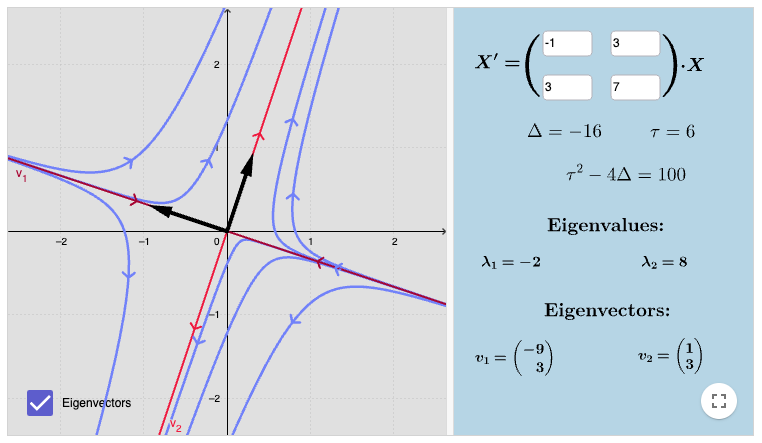
\includegraphics[width=5in]{Images/ImgPhasePlane1337.png}
        \end{center}         
    } 
    \else 
        \begin{center}
        \begin{tikzpicture}[scale=0.85]
        \draw[very thick, ->] (-3, 0) -- (3.25, 0);
        \draw[very thick, ->] (0, -3) -- (0, 3.25);
        \end{tikzpicture}
        \end{center}    
    \fi    

\end{parts}
\fi








\ifnum \Version=9
    \question[6] Consider the IVP $$\vec x \, ' = A\vec x, \quad A = \begin{pmatrix} -2&3\\3&-2 \end{pmatrix}, \quad \vec x = \begin{pmatrix} x(t)\\y(t)\end{pmatrix}, \quad \vec x(0) = \begin{pmatrix} 2\\2 \end{pmatrix}$$ The eigenvalues of $A$ are $\lambda_1 = -5$ and $\lambda_2 = 1$. 
    \begin{parts}
        \part Determine the eigenvectors of $A$. Please show your work. 
        
        \ifnum \Solutions=1 {\color{DarkBlue} 
        \textbf{Solutions:}
        For $\lambda_1$:
        \begin{align}
            A - \lambda_1 I = \begin{pmatrix} 3&3\\3&3\end{pmatrix} \ \Rightarrow \ v_1 = \begin{pmatrix} -1\\1 \end{pmatrix}
        \end{align}
        For $\lambda_2$:
        \begin{align}
            A - \lambda_2 I = \begin{pmatrix} -3&3\\3&-3\end{pmatrix} \ \Rightarrow \ v_2 = \begin{pmatrix} 1\\1 \end{pmatrix}
        \end{align}    
        } 
        \else 
            \vspace{6cm}   
        \fi        
        \part Use the given eigenvalues and the eigenvectors that you calculated in part (a) to solve the IVP.  
        
        \ifnum \Solutions=1 {\color{DarkBlue} 
        \textbf{Solutions:} the general solution to the DE is:
        $$\vec x = c_1 e^{-5t}\begin{pmatrix} -1\\1\end{pmatrix} + c_2e^{t} \begin{pmatrix} 1\\1\end{pmatrix}$$
        Use initial condition:
        \begin{align}
            \begin{pmatrix} 2\\2\end{pmatrix} &= c_1\begin{pmatrix}-1\\1 \end{pmatrix}+ c_2 \begin{pmatrix} 1\\1\end{pmatrix} \ \Rightarrow \ c_1 = 0, c_2 = 2 \ \Rightarrow \ 
            \vec x (t) = 2e^{t} \begin{pmatrix} 1\\1\end{pmatrix}
        \end{align}
        } 
        \else 
        \vspace{7cm}
    \fi
    \part Sketch the phase portrait of the system on the axes below. Please indicate the direction of motion on your solution curves and draw the eigenspaces corresponding to real eigenvalues (if any). Please also label your axes. 
    
    \ifnum \Solutions=1 {\color{DarkBlue} 
    \textbf{Solutions:}
        \begin{center}
        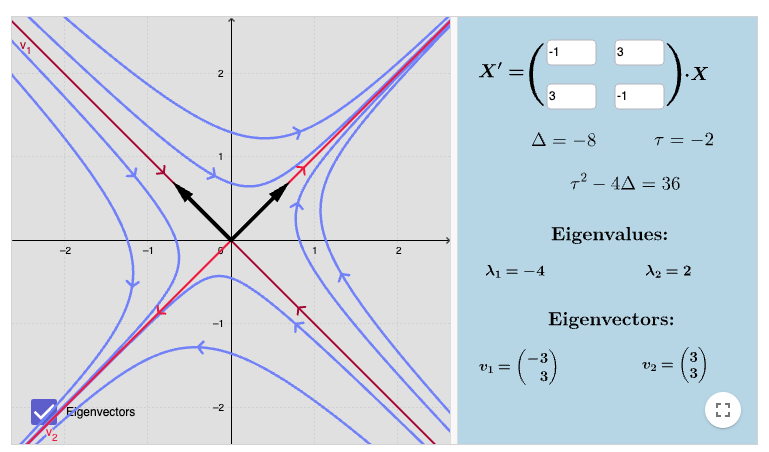
\includegraphics[width=5in]{Images/ImgPhasePlane1331.png}
        \end{center}         
    } 
    \else 
        \begin{center}
        \begin{tikzpicture}[scale=0.85]
        \draw[very thick, ->] (-3, 0) -- (3.25, 0);
        \draw[very thick, ->] (0, -3) -- (0, 3.25);
        \end{tikzpicture}
        \end{center}    
    \fi    

\end{parts}
\fi
    \ifnum \Version=1  
\question[8] Consider the differential equation $\displaystyle \frac{dy}{dt}= (y-2)(y-4k), \ k > 2$. The variable $y$ is a real function of $t$. Assume $y \in  \mathbb R$ and $t \ge 0$.
\fi
\ifnum \Version=2  
\question[8] Consider the differential equation $\displaystyle \frac{dy}{dt}= y^2-9$. The variable $y$ is a real function of $t$. Assume $y \in  \mathbb R$ and $t \ge 0$.
\fi 
\ifnum \Version=3
\question[8] Consider the differential equation $\displaystyle \frac{dy}{dt}= (y-1)(y+2)$. The variable $y$ is a real function of $t$. Assume $y \in  \mathbb R$ and $t \ge 0$.
\fi 
\ifnum \Version=4
\question[8] Consider the differential equation $\displaystyle \frac{dy}{dt}= y^2-4$. The variable $y$ is a real function of $t$. Assume $y \in  \mathbb R$ and $t \ge 0$.
\fi 
\ifnum \Version=5
\question[8] Consider the differential equation $\displaystyle \frac{dy}{dt}= (y+2)(y-3)$. The variable $y$ is a real function of $t$. Assume $y \in  \mathbb R$ and $t \ge 0$.
\fi 

\ifnum \Version<6
\begin{parts}
\part State the critical points of the differential equation.\vspace{1cm}
\part Draw the phase line, and determine whether the critical points (if any) are stable, semi-stable, or unstable.
\vspace{4cm}
\part Determine where $y$ is concave up and where $y$ is concave down for all $y \in \mathbb R$.  Show your work.
\vspace{7cm}
\part Use your results from parts A, B, and C to sketch several solution curves in the $ty$-plane for $y \in \mathbb R$ and $t \ge 0$. Clearly indicate the critical points and the points where the concavity changes. Please label your axes.     
\end{parts}
\fi


\ifnum \Version>5
\question[4] Consider the DE $\displaystyle \dydt = (y-4)(y-8)=y^2-12y+32$. Determine the values of $y$ where the solution curves are concave up and where the curves are concave down. Please show your work. 
\ifnum \Solutions=1 {\color{DarkBlue} 
    \text{Solutions:} Setting $y'=0$ we find that the equilibrium points are $y = 4, 6.$ And if $f(y) = y'$, then $$\dydtt = \dfdy \, \dydt$$ Also 
    $$\dfdy = \ddy\left(y^2-12y+32)\right) = 2y-12 = 2(y-6)$$
    So $df/dy = 0$ when $y=6$. There may be inflection points where either (or both) $df/dy$ and $dy/dt$ are zero. So there could be inflection points at $$y = 4, \ y = 8$$ A table will help determine concavity. When both derivatives have the same sign, the solutions are concave up, and when they have opposite signs the solutions are concave down. 
    \begin{center}            
        \renewcommand{\arraystretch}{1.4}
        \begin{tabular}{c|cccc} 
        $ y $ & $ (-\infty,4) $ & $(4,6)$ & $(6,8)$ & $(8,\infty)$  \\ \hline 
        $\displaystyle  dy/dt=(y-4)(y-8)$ & $+$ & $-$ & $-$ & $+$  \\ \hline
        $ \displaystyle df/dy = 2(y-6) $ & $-$ & $-$ & $+$ & $+$  \\[4pt] \hline
        $ \text{concavity} $ & \text{down} & \text{up} & \text{down} & \text{up} \\ \hline
        \end{tabular}
    \end{center}  
    So concave up on $y>8$ and $4<y<6$. Concave down on $y<4$, and $6<y<8$. 
} 
\else 
\fi
\fi 




        
\end{questions}

% SCRATCH
\ifnum \Solutions=0 \newpage 
    \begin{center}
        \textit{This page can be used for scratch work. }
    \end{center}
\fi
    % VERSION C
    \newpage 
    \renewcommand{\Version}{8} 
    % TEST SPECIFIC INFORMATION
% SAMPLE
\ifnum \Version=1 \renewcommand{\TestName}{Sample Test 1} \fi
% 2023 VERSIONS
\ifnum \Version=2 \renewcommand{\TestName}{Test 1 Version A} \fi
\ifnum \Version=3 \renewcommand{\TestName}{Test 1 Version B} \fi
\ifnum \Version=4 \renewcommand{\TestName}{Test 1 Version C} \fi
\ifnum \Version=5 \renewcommand{\TestName}{Test 1 Version D} \fi
% 2024 VERSIONS
\ifnum \Version=6 \renewcommand{\TestName}{Test 1 Version A} \fi
\ifnum \Version=7 \renewcommand{\TestName}{Test 1 Version B} \fi
\ifnum \Version=8 \renewcommand{\TestName}{Test 1 Version C} \fi
\ifnum \Version=9 \renewcommand{\TestName}{Test 1 Version D} \fi
\ifnum \Version=10 \renewcommand{\TestName}{Test 1 Make-Up} \fi

    % COLORED BOX FORMATTING
    % These boxes are used for definitions and theorems 
    % This code has to appear after begin{document}
    \tikzstyle{mybox} = [draw=black, fill=black!2, very thick, rectangle, rounded corners, inner sep=10pt, inner ysep=10pt]
    \tikzstyle{fancytitle} =[draw=black, very thick, fill=black!6, text=black, rounded corners]

    
% HEADERS AND FOOTERS
\pagestyle{headandfoot}
% \runningfooter{}{}{}
\runningfooter{}{}{\textit{Page \thepage \ of \pageref{LastPage}} }
\runningheader{\textit{Please write your last name: \framebox{\strut\hspace{5cm}} }}{}{\textit{\TestName} }
% \headheight 42pt % distance from top of page to top of header
% \headsep 12pt % space between header and top of body

\vspace*{-1cm}

\begin{center}
{\Large \TestName, \Course}
\end{center}
\renewcommand{\ID}{Please print your first name: \framebox{\strut\hspace{4.2cm}}, last name: \framebox{\strut\hspace{4.2cm}}, \\[2pt] and the remaining digits of your GTID:  \framebox{\strut $9$}\framebox{\strut $0$}\framebox{\strut\hspace{0.19cm}}\framebox{\strut\hspace{0.19cm}}\framebox{\strut\hspace{0.19cm}}\framebox{\strut\hspace{0.19cm}}\framebox{\strut\hspace{0.19cm}}\framebox{\strut\hspace{0.19cm}}\framebox{\strut\hspace{0.19cm}}.}

\ID

\begin{center}
    \setlength{\extrarowheight}{0.25cm}
    {\Large Helpful Formulas} \\
    \vspace{12pt}
    \textbf{Complex Solutions to 2D First Order Systems}
    \begin{align*}
        \lambda &= \alpha + i \beta, \ \beta \ne 0 , \ \vec v = \vec a + i \vec b \\
        \vec x_1 &= e^{\alpha t} (\vec a \cos \beta t - \vec b \sin \beta t), \quad 
        \vec x_{2} = e^{\alpha t} (\vec a \sin \beta t + \vec b \cos \beta t)
    \end{align*}
    \textbf{Repeated Eigenvalues in First Order 2D Systems}
    \begin{align*}
        (A-\lambda I) \vec w &= \vec v, \quad \vec w = t\vec v + \vec c
    \end{align*}    
\end{center}
    \begin{questions}


    \ifnum \Version=1  
\question[4] You do not need to show your work for this question. Consider the differential equation (DE) below.
$$\displaystyle t^2 \, \frac{d^2y}{dt^2} + \dydt = y^4$$
\begin{parts}
    \part Fill in the appropriate circle to indicate whether the DE is linear or non-linear
    \begin{itemize}
        \item[$\bigcirc$] The DE is linear.
        \item[$\bigcirc$] The DE is non-linear.
    \end{itemize}
    \part What is the order of the DE? \framebox{\strut\hspace{2cm}}
    \part Fill in the appropriate circle to indicate whether the DE is autonomous or non-autonomous. 
    \begin{itemize}        
        \item[$\bigcirc$] The DE is autonomous.
        \item[$\bigcirc$] The DE is non-autonomous.
    \end{itemize}    
    \part Is the DE is homogeneous or inhomogeneous? 
    \begin{itemize}        
        \item[$\bigcirc$] The DE is homogeneous.
        \item[$\bigcirc$] The DE is inhomogeneous.
    \end{itemize}        
\end{parts}
\fi 
\ifnum \Version=2
\question[4] You do not need to show your work for this question. Consider the differential equation below.
$$\displaystyle t^3 \, \frac{d^2y}{dt^2} + t\, \dydt + 2y^2 = \cos t$$
\begin{parts}
    \part Indicate whether the DE is homogeneous or inhomogeneous by filling in the appropriate circle. 
    \begin{itemize}        
        \item[$\bigcirc$] The DE is homogeneous.
        \item[$\bigcirc$] The DE is inhomogeneous.
    \end{itemize}     
    \part Fill in the appropriate circle to indicate whether the DE is linear or non-linear
    \begin{itemize}
        \item[$\bigcirc$] The DE is linear.
        \item[$\bigcirc$] The DE is non-linear.
    \end{itemize}
    \part Indicate whether the DE is autonomous or non-autonomous by filling in the appropriate circle. 
    \begin{itemize}        
        \item[$\bigcirc$] The DE is autonomous.
        \item[$\bigcirc$] The DE is non-autonomous.
    \end{itemize}       
    \part What is the order of the DE? \framebox{\strut\hspace{2cm}}
\end{parts}
\fi 

\ifnum \Version=3
\question[4] You do not need to show your work for this question. Consider the differential equation below.
$$\displaystyle 2 \frac{d^2y}{dt^2} + \dydt + 4y = \cos t$$
\begin{parts}
    \part Indicate whether the DE is autonomous or non-autonomous by filling in the appropriate circle. 
    \begin{itemize}        
        \item[$\bigcirc$] The DE is autonomous.
        \item[$\bigcirc$] The DE is non-autonomous.
    \end{itemize}       
    \part Indicate whether the DE is homogeneous or inhomogeneous by filling in the appropriate circle. 
    \begin{itemize}        
        \item[$\bigcirc$] The DE is homogeneous.
        \item[$\bigcirc$] The DE is inhomogeneous.
    \end{itemize}     
    \part Fill in the appropriate circle to indicate whether the DE is linear or non-linear
    \begin{itemize}
        \item[$\bigcirc$] The DE is linear.
        \item[$\bigcirc$] The DE is non-linear.
    \end{itemize}
    \part What is the order of the DE? \framebox{\strut\hspace{2cm}}
\end{parts}
\fi 

\ifnum \Version=4
\question[4] You do not need to show your work for this question. Consider the differential equation below.
$$\displaystyle 2 \frac{d^3y}{dt^3} + \dydt + 4y = t^4$$
\begin{parts}
    \part Indicate whether the DE is autonomous or non-autonomous by filling in the appropriate circle. 
    \begin{itemize}        
        \item[$\bigcirc$] The DE is autonomous.
        \item[$\bigcirc$] The DE is non-autonomous.
    \end{itemize}       
    \part What is the order of the DE? \framebox{\strut\hspace{2cm}} 
    \part Indicate whether the DE is homogeneous or inhomogeneous by filling in the appropriate circle. 
    \begin{itemize}        
        \item[$\bigcirc$] The DE is homogeneous.
        \item[$\bigcirc$] The DE is inhomogeneous.
    \end{itemize}     
    \part Fill in the appropriate circle to indicate whether the DE is linear or non-linear
    \begin{itemize}
        \item[$\bigcirc$] The DE is linear.
        \item[$\bigcirc$] The DE is non-linear.
    \end{itemize}
\end{parts}
\fi 

\ifnum \Version=5
\question[4] You do not need to show your work for this question. Consider the differential equation below.
$$\displaystyle 2 \dydt + 4y^2 = 0$$
\begin{parts}    
    \part What is the order of the DE? \framebox{\strut\hspace{2cm}} 
    \part Indicate whether the DE is homogeneous or inhomogeneous by filling in the appropriate circle. 
    \begin{itemize}        
        \item[$\bigcirc$] The DE is homogeneous.
        \item[$\bigcirc$] The DE is inhomogeneous.
    \end{itemize}     
    \part Fill in the appropriate circle to indicate whether the DE is linear or non-linear
    \begin{itemize}
        \item[$\bigcirc$] The DE is linear.
        \item[$\bigcirc$] The DE is non-linear.
    \end{itemize}
    \part Indicate whether the DE is autonomous or non-autonomous by filling in the appropriate circle. 
    \begin{itemize}        
        \item[$\bigcirc$] The DE is autonomous.
        \item[$\bigcirc$] The DE is non-autonomous.
    \end{itemize}       
\end{parts}
\fi 


\ifnum \Version=6
\question[4] You do not need to show your work for this question. Consider the differential equation below.
$$\displaystyle \dydtt + t^4 \, \frac{dy}{dt} + y = \cos(t)$$    
\begin{parts}
    \part Fill in the appropriate circle to indicate whether the DE is linear or non-linear.
    \begin{itemize}
        \item[$\bigcirc$] The DE is linear.
        \item[$\bigcirc$] The DE is non-linear.
    \end{itemize}
    \part Indicate whether the DE is autonomous or non-autonomous. 
    \begin{itemize}        
        \item[$\bigcirc$] The DE is autonomous.
        \item[$\bigcirc$] The DE is non-autonomous.
    \end{itemize}    
    \part Indicate whether the DE is homogeneous or non-homogeneous. 
    \begin{itemize}        
        \item[$\bigcirc$] The DE is homogeneous.
        \item[$\bigcirc$] The DE is non-homogeneous.
    \end{itemize}    
    \part What is the order of the DE? \framebox{\strut\hspace{4cm}}
    \vspace{2pt}   
    
\end{parts}
\ifnum \Solutions=1 {\color{DarkBlue} 
\textbf{Solutions:}
The DE can be classified as:
\begin{enumerate}
    \item \textbf{linear} because the coefficients are functions of $t$ only
    \item \textbf{not autonomous} because $t$ appears in the coefficients
    \item \textbf{not homogeneous} because of the $\cos t$ term
    \item \textbf{second order} because the highest degree derivative is 2    
\end{enumerate}
} 
\else 
\fi
\fi 




\ifnum \Version=7
\question[4] You do not need to show your work for this question. Consider the differential equation below.
$$\displaystyle \dydttt + t^4 \, \frac{dy}{dt} = y^2$$    
\begin{parts}
    \part Fill in the appropriate circle to indicate whether the DE is linear or non-linear.
    \begin{itemize}
        \item[$\bigcirc$] The DE is linear.
        \item[$\bigcirc$] The DE is non-linear.
    \end{itemize}
    \part Indicate whether the DE is autonomous or non-autonomous. 
    \begin{itemize}        
        \item[$\bigcirc$] The DE is autonomous.
        \item[$\bigcirc$] The DE is non-autonomous.
    \end{itemize}    
    \part Indicate whether the DE is homogeneous or non-homogeneous. 
    \begin{itemize}        
        \item[$\bigcirc$] The DE is homogeneous.
        \item[$\bigcirc$] The DE is non-homogeneous.
    \end{itemize}    
    \part What is the order of the DE? \framebox{\strut\hspace{4cm}}
    \vspace{2pt}   
    
\end{parts}
\ifnum \Solutions=1 {\color{DarkBlue} 
\textbf{Solutions:}
The DE can be classified as:
\begin{enumerate}
    \item \textbf{non-linear} because of the $y^2$ term
    \item \textbf{not autonomous} because $t$ appears in the coefficients
    \item \textbf{homogeneous} because there are no terms that are only functions of $t$
    \item \textbf{third order} because the highest degree derivative is 3  
\end{enumerate}
} 
\else 
\fi
\fi 




\ifnum \Version=8
\question[4] You do not need to show your work for this question. Consider the differential equation below.
$$\displaystyle \dydt + y^2 = t^3$$    
\begin{parts}
    \part Fill in the appropriate circle to indicate whether the DE is linear or non-linear.
    \begin{itemize}
        \item[$\bigcirc$] The DE is linear.
        \item[$\bigcirc$] The DE is non-linear.
    \end{itemize}
    \part Indicate whether the DE is autonomous or non-autonomous. 
    \begin{itemize}        
        \item[$\bigcirc$] The DE is autonomous.
        \item[$\bigcirc$] The DE is non-autonomous.
    \end{itemize}    
    \part Indicate whether the DE is homogeneous or non-homogeneous. 
    \begin{itemize}        
        \item[$\bigcirc$] The DE is homogeneous.
        \item[$\bigcirc$] The DE is non-homogeneous.
    \end{itemize}    
    \part What is the order of the DE? \framebox{\strut\hspace{4cm}}
    \vspace{2pt}   
    
\end{parts}
\ifnum \Solutions=1 {\color{DarkBlue} 
\textbf{Solutions:}
The DE can be classified as:
\begin{enumerate}
    \item \textbf{non-linear} because of the $y^2$ term
    \item \textbf{not autonomous} because $t$ appears in the DE
    \item \textbf{not homogeneous} because there are terms that are only functions of $t$
    \item \textbf{first order} because the highest degree derivative is 1
\end{enumerate}
} 
\else 
\fi
\fi 





\ifnum \Version=9
\question[4] You do not need to show your work for this question. Consider the differential equation below.
$$\displaystyle \dydtt + \dydt + t^3y = 0$$    
\begin{parts}
    \part Fill in the appropriate circle to indicate whether the DE is linear or non-linear.
    \begin{itemize}
        \item[$\bigcirc$] The DE is linear.
        \item[$\bigcirc$] The DE is non-linear.
    \end{itemize}
    \part Indicate whether the DE is autonomous or non-autonomous. 
    \begin{itemize}        
        \item[$\bigcirc$] The DE is autonomous.
        \item[$\bigcirc$] The DE is non-autonomous.
    \end{itemize}    
    \part Indicate whether the DE is homogeneous or non-homogeneous. 
    \begin{itemize}        
        \item[$\bigcirc$] The DE is homogeneous.
        \item[$\bigcirc$] The DE is non-homogeneous.
    \end{itemize}    
    \part What is the order of the DE? \framebox{\strut\hspace{4cm}}
    \vspace{2pt}   
    
\end{parts}
\ifnum \Solutions=1 {\color{DarkBlue} 
\textbf{Solutions:}
The DE can be classified as:
\begin{enumerate}
    \item \textbf{linear} because the coefficients are only functions of $t$
    \item \textbf{not autonomous} because $t$ appears in the DE
    \item \textbf{ homogeneous} because there are no terms that are only functions of $t$
    \item \textbf{second order} because the highest degree derivative is 2
\end{enumerate}
} 
\else 
\fi
\fi 
    \ifnum \Version=1  
\question[2] Consider the autonomous differential equation $\displaystyle \frac{dy}{dt}= (y-1)(y-k^2)$.  Assume $k$ can be any real number. Draw the bifurcation diagram on the axes below. That is, plot the location of the critical points versus $k$. Please label your axes.
        \begin{center}
        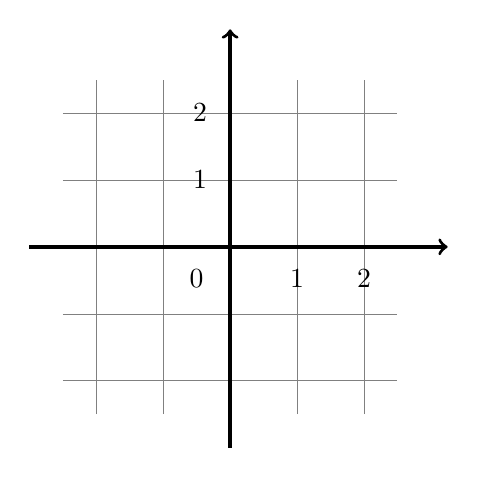
\begin{tikzpicture}[scale=0.85]
        \draw[help lines] (-2.5,-2.5) grid (2.5, 2.5);
        \draw[very thick, ->] (-3, 0) -- (3.25, 0);
        \draw[very thick, ->] (0, -3) -- (0, 3.25);
        \node[overlay, left] at (-0.2, 1) {$1$};
        \node[overlay, left] at (-0.2, 2) {$2$};
        \node[overlay, below] at (-0.5, -0.2) {$0$};
        \node[overlay, below] at (1, -0.2) {$1$};
        \node[overlay, below] at (2, -0.2) {$2$};
        \end{tikzpicture}
        \end{center}
\fi

\ifnum \Version=2
\question[2] Consider the autonomous differential equation $\displaystyle \frac{dy}{dt}= (y-k)(y+1-k^2)$.  Assume $k$ can be any real number. Draw the bifurcation diagram on the axes below. That is, plot the location of the critical points versus $k$. Please label your axes.
        \begin{center}
        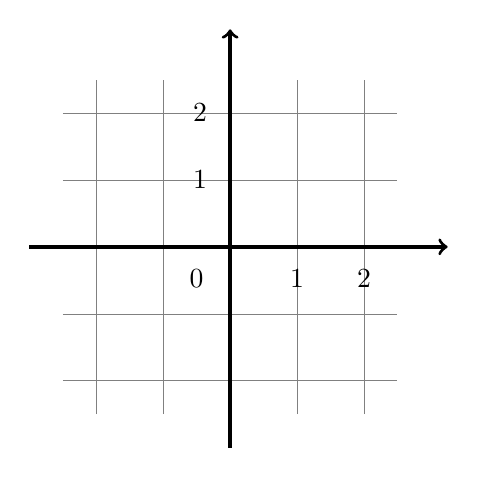
\begin{tikzpicture}[scale=0.85]
        \draw[help lines] (-2.5,-2.5) grid (2.5, 2.5);
        \draw[very thick, ->] (-3, 0) -- (3.25, 0);
        \draw[very thick, ->] (0, -3) -- (0, 3.25);
        \node[overlay, left] at (-0.2, 1) {$1$};
        \node[overlay, left] at (-0.2, 2) {$2$};
        \node[overlay, below] at (-0.5, -0.2) {$0$};
        \node[overlay, below] at (1, -0.2) {$1$};
        \node[overlay, below] at (2, -0.2) {$2$};
        \end{tikzpicture}
        \end{center}
\fi

\ifnum \Version=3
    \question[2] You do not need to show your work for this question. Consider the differential equation 
    \begin{align*}
        t^2y'' - 4ty' - 2y = 12
    \end{align*}
    The DE can be expressed in the form $\vec x\, ' = A\vec x + \vec g$, where 
    \begin{align*}
     A = \left( \hbox to 2cm{\vbox to 0.85cm{}} \right), \quad \vec g = \left( \hbox to 1.2cm{\vbox to 0.85cm{}} \right)
    \end{align*}
    Fill in the missing entries in the above to define $A$ and $\vec g$. 
\fi

\ifnum \Version=4
\question[2] Consider the autonomous differential equation $\displaystyle \frac{dy}{dt}= (y+k)(y^2-k)$.  Assume $k\ge0$. Draw the bifurcation diagram on the axes below. That is, plot the location of the critical points versus $k$. Please label your axes.
        \begin{center}
        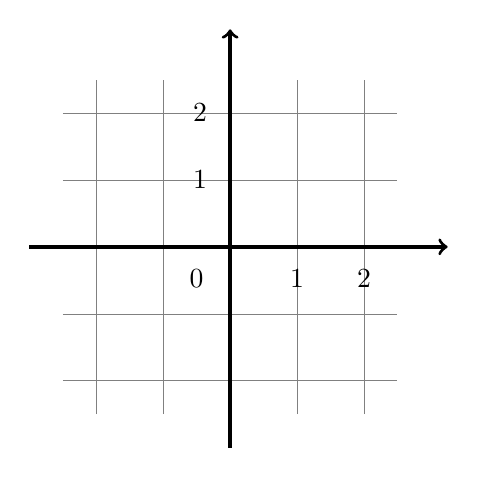
\begin{tikzpicture}[scale=0.85]
        \draw[help lines] (-2.5,-2.5) grid (2.5, 2.5);
        \draw[very thick, ->] (-3, 0) -- (3.25, 0);
        \draw[very thick, ->] (0, -3) -- (0, 3.25);
        \node[overlay, left] at (-0.2, 1) {$1$};
        \node[overlay, left] at (-0.2, 2) {$2$};
        \node[overlay, below] at (-0.5, -0.2) {$0$};
        \node[overlay, below] at (1, -0.2) {$1$};
        \node[overlay, below] at (2, -0.2) {$2$};
        \end{tikzpicture}
        \end{center}
\fi

\ifnum \Version=5
    \question[2] You do not need to show your work for this question. Consider the differential equation 
    \begin{align*}
        4y'' - t^2y' - 2ty = 12\cos(t)
    \end{align*}
    The DE can be expressed in the form $\vec x\, ' = A\vec x + \vec g$, where 
    \begin{align*}
     A = \left( \hbox to 2cm{\vbox to 0.85cm{}} \right), \quad \vec g = \left( \hbox to 1.2cm{\vbox to 0.85cm{}} \right)
    \end{align*}
    Fill in the missing entries in the above to define $A$ and $\vec g$. 
\fi




\ifnum \Version=6
\question[1] You do not need to show your work for this question. Consider the IVP below.
$$\displaystyle y' = \sqrt{4-t^2+y}, \ y(1) = 2$$   
Using the theorems we covered in lecture, fill in all of the appropriate circles below to indicate the intervals over which there must contain a unique solution to the IVP. 
\begin{itemize}
    \item[$\bigcirc$] $y \ge 4-t^2$
    \item[$\bigcirc$] $y \le 4-t^2$
    \item[$\bigcirc$] $y \le t^2-4$
    \item[$\bigcirc$] $y \ge t^2-4$
    \item[$\bigcirc$] none of the above
\end{itemize}
\ifnum \Solutions=1 {\color{DarkBlue} 
\textbf{Solutions:} the relevant theorem is below. 

    \begin{center}\begin{tikzpicture} \node [mybox](box){\begin{minipage}{0.95\textwidth} \vspace{4pt}

    If $f$ and $\frac{\partial f}{\partial y}$ are continuous over $\alpha < t < \beta$, and $\gamma < y < \delta$, which contains the point $(t_0,y_0)$, then there is a unique solution to the IVP $$y' = f(t,y), \quad y(t_0) = y_0$$ on an interval contained in $\alpha < t < \beta$. 
    
    \end{minipage}}; \node[fancytitle, rounded corners, thick, inner sep = 4pt, right=10pt] at (box.north west) {Theorem 2.4.2: Existence and Uniqueness of 1st Order Nonlinear IVP};
    \end{tikzpicture}\end{center}
    
    Taking the partial derivative with respect to $y$:
\begin{align}
    \frac{\partial f}{\partial y} &= \frac{1}{\sqrt{4-t^2+y}}\\
\end{align}
The relevant functions are 
\begin{align}
    f(t,y) &= \sqrt{4-t^2+y} \\
    \frac{\partial f}{\partial y} &= \frac{1}{\sqrt{4-t^2+y}}
\end{align}
They are real and continuous over $$4-t^2+y > 0$$ and this interval also contains $t_0 = 0$ and $y(t_0)$. So the interval over which there must contain a unique solution is $$y > t^2-4$$ 
} 
\else 
\fi
\fi 




\ifnum \Version=7
\question[1] You do not need to show your work for this question. Consider the IVP below.
$$\displaystyle (t+3)y' + \sqrt{4-t^2}\,y = t^4, \ y(1) = 9$$   
Using the theorems we covered in lecture, fill in all of the appropriate circles below to indicate the intervals over which there must contain a unique solution to the IVP. 
\begin{itemize}
    \item[$\bigcirc$] $-3 < t \le 2$
    \item[$\bigcirc$] $-2 \le t \le 2$
    \item[$\bigcirc$] $-2 \le t \le 3$    
    \item[$\bigcirc$] $-\infty \le t < -3$
    \item[$\bigcirc$] none of the above
\end{itemize}
\ifnum \Solutions=1 {\color{DarkBlue} 
\textbf{Solutions:} convert to standard form:
\begin{align}
    y' + \frac{\sqrt{4-t^2}}{t+3}\,y = \frac{t^4}{t+3}
\end{align}
The coefficients are real and continuous over $$-2\le t \le 2$$ and this interval also contains $t_0 = 1$. So the interval over which there must contain a unique solution is $-2\le t \le 2$. 
} 
\else 
\fi
\fi 



\ifnum \Version=8
\question[1] You do not need to show your work for this question. Consider the IVP below.
$$\displaystyle y' = \sqrt{4-t^2-y}, \ y(0) = 2$$   
Using the theorems we covered in lecture, fill in all of the appropriate circles below to indicate the intervals over which there must contain a unique solution to the IVP. 
\begin{itemize}
    \item[$\bigcirc$] $y \ge 4-t^2$
    \item[$\bigcirc$] $y \le 4-t^2$
    \item[$\bigcirc$] $y \le t^2-4$
    \item[$\bigcirc$] $y \ge t^2-4$
    \item[$\bigcirc$] none of the above
\end{itemize}
\ifnum \Solutions=1 {\color{DarkBlue} 
\textbf{Solutions:} partial derivative with respect to $y$:
\begin{align}
    \frac{\partial f}{\partial y} &= \frac{-1}{\sqrt{4-t^2-y}}
\end{align}
The coefficients are real and continuous over $$4-t^2-y\ge 0$$ and this interval also contains $t_0 = 0$ and $y(t_0)$. So the interval over which there must contain a unique solution is $y \le 4-t^2$. 
} 
\else 
\fi
\fi 



\ifnum \Version=9
\question[1] You do not need to show your work for this question. Consider the IVP below.
$$\displaystyle y' = \sqrt{4-t^2+y}, \ y(0) = 2$$   
Using the theorems we covered in lecture, fill in all of the appropriate circles below to indicate the intervals over which there must contain a unique solution to the IVP. 
\begin{itemize}
    \item[$\bigcirc$] $y \ge 4-t^2$
    \item[$\bigcirc$] $y \le 4-t^2$
    \item[$\bigcirc$] $y \le t^2-4$
    \item[$\bigcirc$] $y \ge t^2-4$
    \item[$\bigcirc$] none of the above
\end{itemize}
\ifnum \Solutions=1 {\color{DarkBlue} 
\textbf{Solutions:} partial derivative with respect to $y$:
\begin{align}
    \frac{\partial f}{\partial y} &= \frac{1}{\sqrt{4-t^2+y}}\\
\end{align}
The coefficients are real and continuous over $$4-t^2+y\ge 0$$ and this interval also contains $t_0 = 0$ and $y(t_0)$. So the interval over which there must contain a unique solution is $y \ge t^2-4$. 
} 
\else 
\fi
\fi 




    \ifnum \Version=6
\question[3] Consider the system $$\vec x \, ' = A\vec x, \quad A = \begin{pmatrix} -3&-4\\1&-1 \end{pmatrix}, \quad \vec x = \begin{pmatrix} x(t)\\y(t)\end{pmatrix} $$ The eigenvalues of $A$ are $\lambda = -2\pm i\sqrt 3$. Sketch the phase portrait of the system. Sketch at least two solution curves. Please indicate the direction of motion on your solution curves. Don't forget to label your axes.   

\ifnum \Solutions=1 {\color{DarkBlue} 
\textbf{Solutions:} solution curves should \textbf{spiral towards} the origin and rotate \textbf{counter clockwise}. Axes should be labelled. Ok to only draw only two solution curves. 
    \begin{center}
    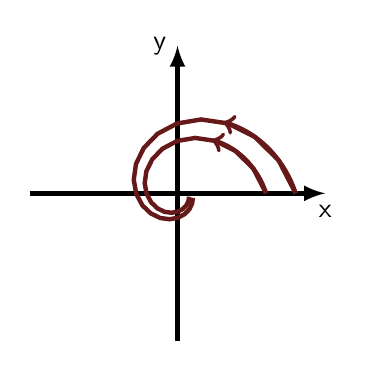
\begin{tikzpicture}[scale=0.75]
      \draw[ultra thick,->,>=latex] (-2.5,0)--(2.5,0) node[below] {x};
      \draw[ultra thick,->,>=latex] (0,-2.5)--(0,2.5) node[left] {y};      
      \draw[domain=0:6,ultra thick,samples=20,DarkRed] plot ({cos(deg(\x))*2*exp(-\x/3},{sin(deg(\x))*2*exp(-\x/3});
      \draw[domain=0:1,->,ultra thick,samples=20,DarkRed] plot ({cos(deg(\x))*2*exp(-\x/3},{sin(deg(\x))*2*exp(-\x/3});
      \draw[domain=0:6,ultra thick,samples=20,DarkRed] plot ({.75*cos(deg(\x))*2*exp(-\x/3},{.75*sin(deg(\x))*2*exp(-\x/3});
      \draw[domain=0:1,->,ultra thick,samples=20,DarkRed] plot ({.75*cos(deg(\x))*2*exp(-\x/3},{.75*sin(deg(\x))*2*exp(-\x/3});
    \end{tikzpicture}
    \end{center} 
} 
\else 
    \begin{center}
    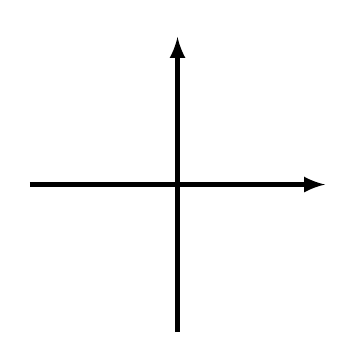
\begin{tikzpicture}[scale=0.75]
      \draw[ultra thick,->,>=latex] (-2.5,0)--(2.5,0) node[below] {};
      \draw[ultra thick,->,>=latex] (0,-2.5)--(0,2.5) node[left] {};         
    \end{tikzpicture}
    \end{center} 
\fi
\fi


\ifnum \Version=7
\question[3] Consider the system $$\vec x \, ' = A\vec x, \quad A = \begin{pmatrix} 3&2\\-5&1 \end{pmatrix}, \quad \vec x = \begin{pmatrix} x(t)\\y(t)\end{pmatrix} $$ The eigenvalues of $A$ are $\lambda = 2\pm  3i$. Sketch the phase portrait of the system. Sketch at least two solution curves. Please indicate the direction of motion on your solution curves. Don't forget to label your axes.   

\ifnum \Solutions=1 {\color{DarkBlue} 
\textbf{Solutions:} solution curves should \textbf{spiral away} from the origin and rotate \textbf{clockwise}. Axes should be labelled. Ok to only draw only two solution curves. 
\begin{center}
    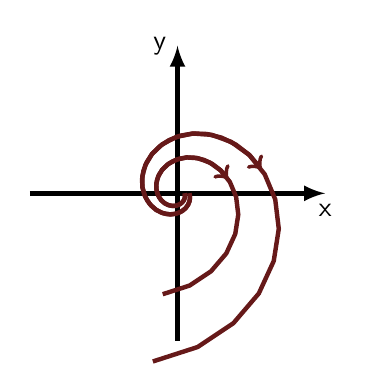
\begin{tikzpicture}[scale=0.75]
      \draw[ultra thick,->,>=latex] (-2.5,0)--(2.5,0) node[below] {x};
      \draw[ultra thick,->,>=latex] (0,-2.5)--(0,2.5) node[left] {y};      
      \draw[domain=0:8,ultra thick,samples=30,DarkRed] plot ({cos(deg(\x))*0.12*exp(\x/3)},{-sin(deg(\x))*0.12*exp(\x/3)});
      \draw[domain=0:6,->,ultra thick,samples=30,DarkRed] plot ({cos(deg(\x))*0.12*exp(\x/3)},{-sin(deg(\x))*0.12*exp(\x/3)});
      \draw[domain=0:8,ultra thick,samples=30,DarkRed] plot ({cos(deg(\x))*0.2*exp(\x/3)},{-sin(deg(\x))*0.2*exp(\x/3)});
      \draw[domain=0:6,->,ultra thick,samples=30,DarkRed] plot ({cos(deg(\x))*0.2*exp(\x/3)},{-sin(deg(\x))*0.2*exp(\x/3)});      
    \end{tikzpicture}
\end{center} 
} 
\else 
\begin{center}
    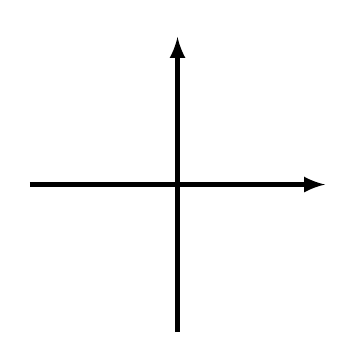
\begin{tikzpicture}[scale=0.75]
      \draw[ultra thick,->,>=latex] (-2.5,0)--(2.5,0) node[below] {};
      \draw[ultra thick,->,>=latex] (0,-2.5)--(0,2.5) node[left] {};         
    \end{tikzpicture}
\end{center} 
\fi
\fi






\ifnum \Version=8
\question[3] Consider the system $$\vec x \, ' = A\vec x, \quad A = \begin{pmatrix} -3&-4\\1&-1 \end{pmatrix}, \quad \vec x = \begin{pmatrix} x(t)\\y(t)\end{pmatrix} $$ The eigenvalues of $A$ are $\lambda = -2\pm i\sqrt 3$. Sketch the phase portrait of the system. Sketch at least two solution curves. Please indicate the direction of motion on your solution curves. Don't forget to label your axes.   

\ifnum \Solutions=1 {\color{DarkBlue} 
\textbf{Solutions:} solution curves should spiral towards center and rotate counter clockwise. Axes should be labelled. Ok to only draw only two solution curves. 
    \begin{center}
    \begin{tikzpicture}[scale=0.75]
      \draw[ultra thick,->,>=latex] (-2.5,0)--(2.5,0) node[below] {x};
      \draw[ultra thick,->,>=latex] (0,-2.5)--(0,2.5) node[left] {y};      
      \draw[domain=0:6,ultra thick,samples=20,DarkRed] plot ({cos(deg(\x))*2*exp(-\x/3},{sin(deg(\x))*2*exp(-\x/3});
      \draw[domain=0:1,->,ultra thick,samples=20,DarkRed] plot ({cos(deg(\x))*2*exp(-\x/3},{sin(deg(\x))*2*exp(-\x/3});
      \draw[domain=0:6,ultra thick,samples=20,DarkRed] plot ({.75*cos(deg(\x))*2*exp(-\x/3},{.75*sin(deg(\x))*2*exp(-\x/3});
      \draw[domain=0:1,->,ultra thick,samples=20,DarkRed] plot ({.75*cos(deg(\x))*2*exp(-\x/3},{.75*sin(deg(\x))*2*exp(-\x/3});
    \end{tikzpicture}
    \end{center} 
} 
\else 
    \begin{center}
    \begin{tikzpicture}[scale=0.75]
      \draw[ultra thick,->,>=latex] (-2.5,0)--(2.5,0) node[below] {};
      \draw[ultra thick,->,>=latex] (0,-2.5)--(0,2.5) node[left] {};         
    \end{tikzpicture}
    \end{center} 
\fi
\fi




\ifnum \Version=9
\question[3] Consider the system $$\vec x \, ' = A\vec x, \quad A = \begin{pmatrix} 1&-4\\1&3 \end{pmatrix}, \quad \vec x = \begin{pmatrix} x(t)\\y(t)\end{pmatrix} $$ The eigenvalues of $A$ are $\lambda = 2\pm i\sqrt 3$. Sketch the phase portrait of the system. Sketch at least two solution curves. Please indicate the direction of motion on your solution curves. Don't forget to label your axes.   

\ifnum \Solutions=1 {\color{DarkBlue} 
\textbf{Solutions:} solution curves should spiral away from the origin and rotate counter clockwise. Axes should be labelled. Ok to only draw only two solution curves. 
    \begin{center}
    \begin{tikzpicture}[scale=0.75]
      \draw[ultra thick,->,>=latex] (-2.5,0)--(2.5,0) node[below] {x};
      \draw[ultra thick,->,>=latex] (0,-2.5)--(0,2.5) node[left] {y};      
      \draw[domain=0:8,ultra thick,samples=30,DarkRed] plot ({cos(deg(\x))*0.12*exp(\x/3)},{sin(deg(\x))*0.12*exp(\x/3)});
      \draw[domain=0:4,->,ultra thick,samples=30,DarkRed] plot ({cos(deg(\x))*0.12*exp(\x/3)},{sin(deg(\x))*0.12*exp(\x/3)});
      \draw[domain=0:8,ultra thick,samples=30,DarkRed] plot ({cos(deg(\x))*0.2*exp(\x/3)},{sin(deg(\x))*0.2*exp(\x/3)});
      \draw[domain=0:4,->,ultra thick,samples=30,DarkRed] plot ({cos(deg(\x))*0.2*exp(\x/3)},{sin(deg(\x))*0.2*exp(\x/3)});      
    \end{tikzpicture}
    \end{center} 
} 
\else 
    \begin{center}
    \begin{tikzpicture}[scale=0.75]
      \draw[ultra thick,->,>=latex] (-2.5,0)--(2.5,0) node[below] {};
      \draw[ultra thick,->,>=latex] (0,-2.5)--(0,2.5) node[left] {};         
    \end{tikzpicture}
    \end{center} 
\fi
\fi



    
\ifnum \Version>5
\question[3] A tank originally contains 50 L of water with 6 kg of salt. Water containing $\frac{1}{20}$ kg of salt per litre is entering at a rate of 4 L/hour, and the well-stirred solution in the tank is leaving at 1 L/hour. 

\begin{parts}
    \part Write down an IVP for $V(t)$, which is the amount of fluid in the tank at time $t$. You do not need to solve your IVP. 
    
    \ifnum \Solutions=1 {\color{DarkBlue} 
        The volume of fluid in the tank is
        $$V = 50 + 3t$$
        By differentiating, the IVP for $V(t)$ is
        $$\frac{dV}{dt} = 3, \quad V(0) = 50$$
        }
    \else
    \vspace{6cm}
    \fi
    
    \part Write down an IVP for $Q(t)$, for the amount of salt in the tank. You do not need to solve the IVP. 
    
    \ifnum \Solutions=1 {\color{DarkBlue} 
        The DE is
        \begin{align}
            \frac{dQ}{dt} &= \left( \text{rate salt coming in} \right) - \left( \text{rate of salt going out} \right) \\
            \frac{dQ}{dt} &= 4\cdot \frac{1}{20} - \frac{Q}{V}
        \end{align}
        The IVP is
        \begin{align}
            \frac{dQ}{dt} &= \frac{1}{5} - \frac{Q}{50+3t}, \quad Q(0) = 6
        \end{align}        
        }
        \fi
    \fi
    
\end{parts}


        

    \newpage        
    \newpage 
\ifnum \Version=1  
\question[4] Solve the initial value problem and solve for $y$ to obtain an explicit expression for $y$ in terms of $t$. Please show your work.
$$\displaystyle t\,\frac{dy}{dt} = \frac{\cos(t)}{t^2} - 3y, \quad y(\pi) = 2, \quad t > 0$$.
\fi

\ifnum \Version=2
\question[4] Solve the initial value problem and solve for $y$ to obtain an explicit expression for $y$ in terms of $t$. Please show your work.
$$\displaystyle \frac{dy}{dt} = 12e^{3t}e^{-2y}, \quad y(0) = 2, \quad t \ge 0$$.
\fi

\ifnum \Version=3
\question[4] Solve the initial value problem and solve for $y$ to obtain an explicit expression for $y$ in terms of $t$. Please show your work.
$$\displaystyle t\,\frac{dy}{dt} + 3y =  36 t^{-2}e^{-t}, \ y(1) = 0, \quad t > 0$$.
\fi   

\ifnum \Version=4
\question[4] Solve the initial value problem and solve for $y$ to obtain an expression for $y$ in terms of $t$. Please show your work.
$$\displaystyle \frac{dy}{dt} = \frac{16e^{2t}}{y}, \quad y(1) = 2, \quad t > 0$$.
\fi

\ifnum \Version=5
\question[4] Solve the initial value problem and solve for $y$ to obtain an explicit expression for $y$ in terms of $t$. Please show your work.
$$\displaystyle t\,\frac{dy}{dt} + 2y =  36 t^{-1}e^{t}, \ y(1) = 2e, \quad t > 0$$.
\fi   



\ifnum \Version=6
\question[4] 
Solve the initial value problem and solve for $y$ to obtain an explicit expression for $y$ in terms of $t$. Please show your work.
$$\displaystyle t\,\frac{dy}{dt} + 4y =  24 t^{-3}e^{2t}, \ y(1) = 2, \quad t > 0$$.

\ifnum \Solutions=1 {\color{DarkBlue} 
\textbf{Solutions:}
To solve the differential equation \( t y' + 4 y = 24 t^{-3} e^{2t} \) with the initial condition \( y(1) = 2 \), we can follow these steps.
\begin{enumerate}
    \item Rewrite the DE in standard form:
   \[ y' + \frac{4}{t} y = 24 t^{-4} e^{2t} \]
   \item Integrating factor:
   \[ \mu(t) = e^{\int \frac{4}{t} \, dt} = e^{4 \ln |t|} = t^4 \]
   \item Multiply both sides of the differential equation by the integrating factor:
   \begin{align*}
       t^4 y' + 4 t^3 y &= 24 e^{2t} \\
       \frac{d}{dt} (t^4 y) &= 24 e^{2t}
   \end{align*} 
   \item Integrate both sides with respect to \( t \) and solve for $y$:
   \begin{align}
       t^4 y &= \int 24 e^{2t} \, dt + C \\
       t^4 y &= 12 e^{2t} + C \\
        y &= \frac{12 e^{2t} + C}{t^4} 
   \end{align} 
   \item Apply the initial condition \( y(1) = 2 \):
   \[ 2 = \frac{12 e^{2 \cdot 1} + C}{1^4} \]
   \[ 2 = 12 e^2 + C \]
   \[ C = 2 - 12 e^2 \]
   \item Substitute \( C \) back into the solution:
   \[ y = \frac{12 e^{2t} + 2 - 12 e^2}{t^4} \]
\end{enumerate}
} 
\else 
\newpage
\fi
\fi   





\ifnum \Version=7
\question[4] 
Solve the initial value problem and solve for $y$ to obtain an explicit expression for $y$ in terms of $t$. Please show your work.
$$\displaystyle t\,\frac{dy}{dt} + 5y =  20 t^{-4}e^{2t}, \ y(1) = e^2, \quad t > 0$$.

\ifnum \Solutions=1 {\color{DarkBlue} 
\textbf{Solutions:}
To solve the differential equation \( t y' + 5 y = 20 t^{-3} e^{2t} \) with the initial condition \( y(1) = 2 \), we can follow these steps.
\begin{enumerate}
    \item Rewrite the DE in standard form:
   \[ y' + \frac{5}{t} y = 20 t^{-4} e^{2t} \]
   \item Integrating factor:
   \[ \mu(t) = e^{\int \frac{5}{t} \, dt} = e^{5 \ln |t|} = t^5 \]
   \item Multiply both sides of the differential equation by the integrating factor:
   \begin{align*}
       t^5 y' + 5 t^4 y &= 20 e^{2t} \\
       \frac{d}{dt} (t^5 y) &= 20 e^{2t}
   \end{align*} 
   \item Integrate both sides with respect to \( t \) and solve for $y$:
   \begin{align}
       t^5 y &= \int 20 e^{2t} \, dt + C \\
       t^5 y &= 10 e^{2t} + C \\
        y &= \frac{10 e^{2t} + C}{t^5} 
   \end{align} 
   \item Apply the initial condition \( y(1) = e^2 \):
   \[ e^2 = \frac{10 e^{2 \cdot 1} + C}{1^5} \]
   \[ e^2 = 10 e^2 + C \]
   \[ C = - 9 e^2 \]
   \item Substitute \( C \) back into the solution:
   \[ y = \frac{10 e^{2t} - 9 e^2}{t^5} \]
\end{enumerate}
} 
\else 
\newpage
\fi
\fi   






\ifnum \Version=8
\question[4] 
Solve the initial value problem and solve for $y$ to obtain an explicit expression for $y$ in terms of $t$. Please show your work.
$$\displaystyle t\,\frac{dy}{dt} + 6y =  24 t^{-5}e^{4t}, \ y(1) = 8e^4, \quad t > 0$$.

\ifnum \Solutions=1 {\color{DarkBlue} 
\textbf{Solutions:}
To solve the DE with the given initial condition we can follow these steps.
\begin{enumerate}
    \item Rewrite the DE in standard form:
   \[ y' + \frac{6}{t} y = 24 t^{-6} e^{4t} \]
   \item Integrating factor:
   \[ \mu(t) = e^{\int \frac{6}{t} \, dt} = e^{6 \ln |t|} = t^6 \]
   \item Multiply both sides of the differential equation by the integrating factor:
   \begin{align*}
       t^6 y' + 6 t^5 y &= 24 e^{4t} \\
       \frac{d}{dt} (t^6 y) &= 24 e^{4t}
   \end{align*} 
   \item Integrate both sides with respect to \( t \) and solve for $y$:
   \begin{align}
       t^6 y &= \int 24 e^{4t} \, dt + C \\
       t^6 y &= 6 e^{4t} + C \\
        y &= \frac{6 e^{4t} + C}{t^6} 
   \end{align} 
   \item Apply the initial condition:
   \[ 8e^4 = \frac{6 e^{4 \cdot 1} + C}{1^5} \]
   \[ 8e^4 = 6 e^4 + C \]
   \[ C = 2 e^4 \]
   \item Substitute \( C \) back into the solution:
   \[ y = \frac{6 e^{4t} +2 e^4}{t^6} \]
\end{enumerate}
} 
\else 
\newpage
\fi
\fi   



\ifnum \Version=9
\question[4] 
Solve the initial value problem and solve for $y$ to obtain an explicit expression for $y$ in terms of $t$. Please show your work.
$$\displaystyle t\,\frac{dy}{dt} + 5y =  20 t^{-4}e^{2t}, \ y(1) = e^2, \quad t > 0$$.

\ifnum \Solutions=1 {\color{DarkBlue} 
\textbf{Solutions:}
To solve the differential equation \( t y' + 5 y = 20 t^{-3} e^{2t} \) with the initial condition \( y(1) = 2 \), we can follow these steps.
\begin{enumerate}
    \item Rewrite the DE in standard form:
   \[ y' + \frac{5}{t} y = 20 t^{-4} e^{2t} \]
   \item Integrating factor:
   \[ \mu(t) = e^{\int \frac{5}{t} \, dt} = e^{5 \ln |t|} = t^5 \]
   \item Multiply both sides of the differential equation by the integrating factor:
   \begin{align*}
       t^5 y' + 5 t^4 y &= 20 e^{2t} \\
       \frac{d}{dt} (t^5 y) &= 20 e^{2t}
   \end{align*} 
   \item Integrate both sides with respect to \( t \) and solve for $y$:
   \begin{align}
       t^5 y &= \int 20 e^{2t} \, dt + C \\
       t^5 y &= 10 e^{2t} + C \\
        y &= \frac{10 e^{2t} + C}{t^5} 
   \end{align} 
   \item Apply the initial condition \( y(1) = e^2 \):
   \[ e^2 = \frac{10 e^{2 \cdot 1} + C}{1^5} \]
   \[ e^2 = 10 e^2 + C \]
   \[ C = - 9 e^2 \]
   \item Substitute \( C \) back into the solution:
   \[ y = \frac{10 e^{2t} - 9 e^2}{t^5} \]
\end{enumerate}
} 
\else 
\newpage
\fi
\fi   
        
    \newpage 

\ifnum \Version=1  
\question[7] Consider the system $$\vec x \, ' = A\vec x, \quad A = \begin{pmatrix} 0&3\\5&2 \end{pmatrix}, \quad \vec x = \begin{pmatrix} x(t)\\y(t)\end{pmatrix} $$.
\begin{parts}
    \part Determine the eigenvalues of $A$. Please show your work. \vspace{5cm}
    \part Determine the eigenvectors of $A$. Please show your work. \vspace{7cm}
    \part Sketch the phase portrait of the system on the axes below. Please indicate the direction of motion on your solution curves and draw the eigenspaces corresponding to real eigenvalues (if any). Please also label your axes. 
    \begin{center}
    \begin{tikzpicture}[scale=0.85]
    \draw[very thick, ->] (-3, 0) -- (3.25, 0);
    \draw[very thick, ->] (0, -3) -- (0, 3.25);
    \end{tikzpicture}
    \end{center}
\end{parts}
\fi

\ifnum \Version=2
\question[7] Consider the system $$\vec x \, ' = A\vec x, \quad A = \begin{pmatrix} 4&3\\3&-4 \end{pmatrix}, \quad \vec x = \begin{pmatrix} x(t)\\y(t)\end{pmatrix} $$.
\begin{parts}
    \part Determine the eigenvalues of $A$. Please show your work. \vspace{5cm}
    \part Determine the eigenvectors of $A$. Please show your work. \vspace{7cm}
    \part Sketch the phase portrait of the system on the axes below. Please indicate the direction of motion on your solution curves and draw the eigenspaces corresponding to real eigenvalues (if any). Please also label your axes. 
    \begin{center}
    \begin{tikzpicture}[scale=0.85]
    \draw[very thick, ->] (-3, 0) -- (3.25, 0);
    \draw[very thick, ->] (0, -3) -- (0, 3.25);
    \end{tikzpicture}
    \end{center}
\end{parts}
\fi

\ifnum \Version=3
\question[7] Consider the system $$\vec x \, ' = A\vec x, \quad A = \begin{pmatrix} 5&4\\-3&-3 \end{pmatrix}, \quad \vec x = \begin{pmatrix} x(t)\\y(t)\end{pmatrix} $$.
\begin{parts}
    \part Determine the eigenvalues of $A$. Please show your work. \vspace{5cm}
    \part Determine the eigenvectors of $A$. Please show your work. \vspace{7cm}
    \part Sketch the phase portrait of the system on the axes below. Please indicate the direction of motion on your solution curves and draw the eigenspaces corresponding to real eigenvalues (if any). Please also label your axes. 
    \begin{center}
    \begin{tikzpicture}[scale=0.85]
    \draw[very thick, ->] (-3, 0) -- (3.25, 0);
    \draw[very thick, ->] (0, -3) -- (0, 3.25);
    \end{tikzpicture}
    \end{center}
\end{parts}
\fi

\ifnum \Version=4
\question[7] Consider the system $$\vec x \, ' = A\vec x, \quad A = \begin{pmatrix} 3&4\\-3&-5 \end{pmatrix}, \quad \vec x = \begin{pmatrix} x(t)\\y(t)\end{pmatrix} $$.
\begin{parts}
    \part Determine the eigenvalues of $A$. Please show your work. \vspace{5cm}
    \part Determine the eigenvectors of $A$. Please show your work. \vspace{7cm}
    \part Sketch the phase portrait of the system on the axes below. Please indicate the direction of motion on your solution curves and draw the eigenspaces corresponding to real eigenvalues (if any). Please also label your axes. 
    \begin{center}
    \begin{tikzpicture}[scale=0.85]
    \draw[very thick, ->] (-3, 0) -- (3.25, 0);
    \draw[very thick, ->] (0, -3) -- (0, 3.25);
    \end{tikzpicture}
    \end{center}
\end{parts}
\fi

\ifnum \Version=5
\question[7] Consider the system $$\vec x \, ' = A\vec x, \quad A = \begin{pmatrix} 4&4\\-3&-4 \end{pmatrix}, \quad \vec x = \begin{pmatrix} x(t)\\y(t)\end{pmatrix} $$.
\begin{parts}
    \part Determine the eigenvalues of $A$. Please show your work. \vspace{5cm}
    \part Determine the eigenvectors of $A$. Please show your work. \vspace{7cm}
    \part Sketch the phase portrait of the system on the axes below. Please indicate the direction of motion on your solution curves and draw the eigenspaces corresponding to real eigenvalues (if any). Please also label your axes. 
    \begin{center}
    \begin{tikzpicture}[scale=0.85]
    \draw[very thick, ->] (-3, 0) -- (3.25, 0);
    \draw[very thick, ->] (0, -3) -- (0, 3.25);
    \end{tikzpicture}
    \end{center}
\end{parts}
\fi



\ifnum \Version=6
    \question[6] Consider the IVP $$\vec x \, ' = A\vec x, \quad A = \begin{pmatrix} -1&3\\3&-1 \end{pmatrix}, \quad \vec x = \begin{pmatrix} x(t)\\y(t)\end{pmatrix}, \quad \vec x(0) = \begin{pmatrix} 2\\2 \end{pmatrix}$$ The eigenvalues of $A$ are $\lambda_1 = -4$ and $\lambda_2 = 2$. 
    \begin{parts}
        \part Determine the eigenvectors of $A$. Please show your work. 
        
        \ifnum \Solutions=1 {\color{DarkBlue} 
        \textbf{Solutions:}
        For $\lambda_1$:
        \begin{align}
            A - \lambda_1 I = \begin{pmatrix} 3&3\\3&3\end{pmatrix} \ \Rightarrow \ v_1 = \begin{pmatrix} -1\\1 \end{pmatrix}
        \end{align}
        For $\lambda_2$:
        \begin{align}
            A - \lambda_2 I = \begin{pmatrix} -3&3\\3&-3\end{pmatrix} \ \Rightarrow \ v_2 = \begin{pmatrix} 1\\1 \end{pmatrix}
        \end{align}    
        } 
        \else 
            \vspace{6cm}   
        \fi        
        \part Use the given eigenvalues and the eigenvectors that you calculated in part (a) to solve the IVP.  
        
        \ifnum \Solutions=1 {\color{DarkBlue} 
        \textbf{Solutions:} the general solution to the DE is:
        $$\vec x = c_1 e^{-4t}\begin{pmatrix} -1\\1\end{pmatrix} + c_2e^{2t} \begin{pmatrix} 1\\1\end{pmatrix}$$
        Use initial condition:
        \begin{align}
            \begin{pmatrix} 2\\2\end{pmatrix} &= c_1\begin{pmatrix}-1\\1 \end{pmatrix}+ c_2 \begin{pmatrix} 1\\1\end{pmatrix} \ \Rightarrow \ c_1 = 0, c_2 = 2 \ \Rightarrow \ 
            \vec x (t) = 2e^{2t} \begin{pmatrix} 1\\1\end{pmatrix}
        \end{align}
        } 
        \else 
        \vspace{7cm}
    \fi
    \part Sketch the phase portrait of the system on the axes below. Please indicate the direction of motion on your solution curves and draw the eigenspaces corresponding to real eigenvalues (if any). Please also label your axes. 
    
    \ifnum \Solutions=1 {\color{DarkBlue} 
    \textbf{Solutions:}
        \begin{center}
        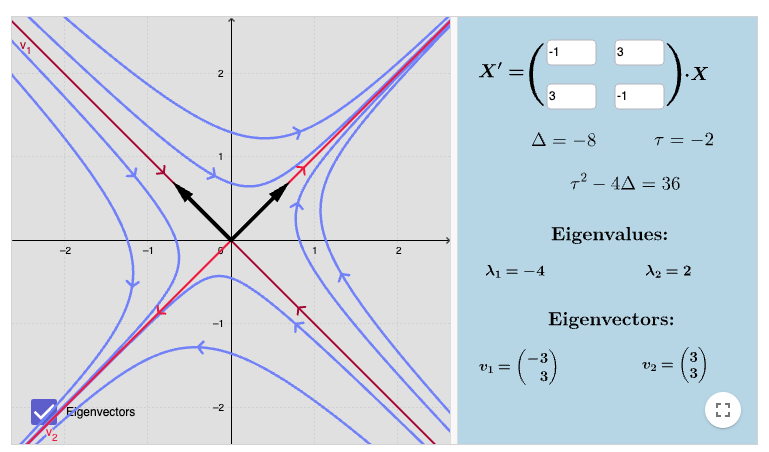
\includegraphics[width=5in]{Images/ImgPhasePlane1331.png}
        \end{center}         
    } 
    \else 
        \begin{center}
        \begin{tikzpicture}[scale=0.85]
        \draw[very thick, ->] (-3, 0) -- (3.25, 0);
        \draw[very thick, ->] (0, -3) -- (0, 3.25);
        \end{tikzpicture}
        \end{center}    
    \fi    

\end{parts}
\fi





\ifnum \Version=7
    \question[6] Consider the IVP $$\vec x \, ' = A\vec x, \quad A = \begin{pmatrix} 0&3\\3&8 \end{pmatrix}, \quad \vec x = \begin{pmatrix} x(t)\\y(t)\end{pmatrix}, \quad \vec x(0) = \begin{pmatrix} -3\\1 \end{pmatrix}$$ The eigenvalues of $A$ are $\lambda_1 = -1$ and $\lambda_2 = 9$. 
    \begin{parts}
        \part Determine the eigenvectors of $A$. Please show your work. 
        
        \ifnum \Solutions=1 {\color{DarkBlue} 
        \textbf{Solutions:}
        For $\lambda_1$:
        \begin{align}
            A - \lambda_1 I = \begin{pmatrix} 1&3\\3&9\end{pmatrix} \ \Rightarrow \ v_1 = \begin{pmatrix} -3\\1 \end{pmatrix}
        \end{align}
        For $\lambda_2$:
        \begin{align}
            A - \lambda_2 I = \begin{pmatrix} -9&3\\3&-1\end{pmatrix} \ \Rightarrow \ v_2 = \begin{pmatrix} 1\\3 \end{pmatrix}
        \end{align}    
        } 
        \else 
            \vspace{6cm}   
        \fi        
        \part Use the given eigenvalues and the eigenvectors that you calculated in part (a) to solve the IVP.  
        
        \ifnum \Solutions=1 {\color{DarkBlue} 
        \textbf{Solutions:} the general solution to the DE is:
        $$\vec x = c_1 e^{-t}\begin{pmatrix} -3\\1\end{pmatrix} + c_2e^{9t} \begin{pmatrix} 1\\3\end{pmatrix}$$
        Use initial condition:
        \begin{align}
            \begin{pmatrix} -3\\1\end{pmatrix} &= c_1\begin{pmatrix}-3\\1 \end{pmatrix}+ c_2 \begin{pmatrix} 1\\3\end{pmatrix} \ \Rightarrow \ c_1 = 1, c_2 = 0 \ \Rightarrow \ 
            \vec x (t) = e^{-t} \begin{pmatrix} -3\\1\end{pmatrix}
        \end{align}
        } 
        \else 
        \vspace{7cm}
    \fi
    \part Sketch the phase portrait of the system on the axes below. Please indicate the direction of motion on your solution curves and draw the eigenspaces corresponding to real eigenvalues (if any). Please also label your axes. 
    
    \ifnum \Solutions=1 {\color{DarkBlue} 
    \textbf{Solutions:}
        \begin{center}
        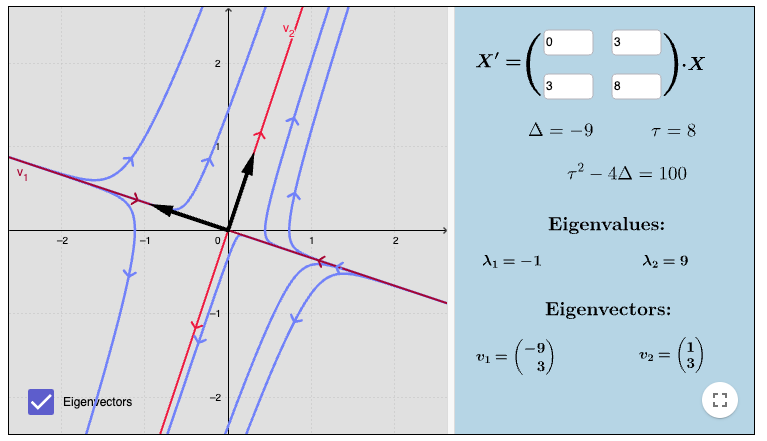
\includegraphics[width=5in]{Images/ImgPhasePlane0338.png}
        \end{center}         
    } 
    \else 
        \begin{center}
        \begin{tikzpicture}[scale=0.85]
        \draw[very thick, ->] (-3, 0) -- (3.25, 0);
        \draw[very thick, ->] (0, -3) -- (0, 3.25);
        \end{tikzpicture}
        \end{center}    
    \fi    

\end{parts}
\fi








\ifnum \Version=8
    \question[6] Consider the IVP $$\vec x \, ' = A\vec x, \quad A = \begin{pmatrix} -1&3\\3&7 \end{pmatrix}, \quad \vec x = \begin{pmatrix} x(t)\\y(t)\end{pmatrix}, \quad \vec x(0) = \begin{pmatrix} 1\\3 \end{pmatrix}$$ The eigenvalues of $A$ are $\lambda_1 = -2$ and $\lambda_2 = 8$. 
    \begin{parts}
        \part Determine the eigenvectors of $A$. Please show your work. 
        
        \ifnum \Solutions=1 {\color{DarkBlue} 
        \textbf{Solutions:}
        For $\lambda_1$:
        \begin{align}
            A - \lambda_1 I = \begin{pmatrix} 1&3\\3&9\end{pmatrix} \ \Rightarrow \ v_1 = \begin{pmatrix} -3\\1 \end{pmatrix}
        \end{align}
        For $\lambda_2$:
        \begin{align}
            A - \lambda_2 I = \begin{pmatrix} -9&3\\3&-1\end{pmatrix} \ \Rightarrow \ v_2 = \begin{pmatrix} 1\\3 \end{pmatrix}
        \end{align}    
        } 
        \else 
            \vspace{6cm}   
        \fi        
        \part Use the given eigenvalues and the eigenvectors that you calculated in part (a) to solve the IVP.  
        
        \ifnum \Solutions=1 {\color{DarkBlue} 
        \textbf{Solutions:} the general solution to the DE is:
        $$\vec x = c_1 e^{-4t}\begin{pmatrix} -1\\1\end{pmatrix} + c_2e^{2t} \begin{pmatrix} 1\\1\end{pmatrix}$$
        Use initial condition:
        \begin{align}
            \begin{pmatrix} 1\\3\end{pmatrix} &= c_1\begin{pmatrix}-3\\1 \end{pmatrix}+ c_2 \begin{pmatrix} 1\\3\end{pmatrix} \ \Rightarrow \ c_1 = 0, c_2 = 1 \ \Rightarrow \ 
            \vec x (t) = e^{8t} \begin{pmatrix} 1\\3\end{pmatrix}
        \end{align}
        } 
        \else 
        \vspace{7cm}
    \fi
    \part Sketch the phase portrait of the system on the axes below. Please indicate the direction of motion on your solution curves and draw the eigenspaces corresponding to real eigenvalues (if any). Please also label your axes. 
    
    \ifnum \Solutions=1 {\color{DarkBlue} 
    \textbf{Solutions:}
        \begin{center}
        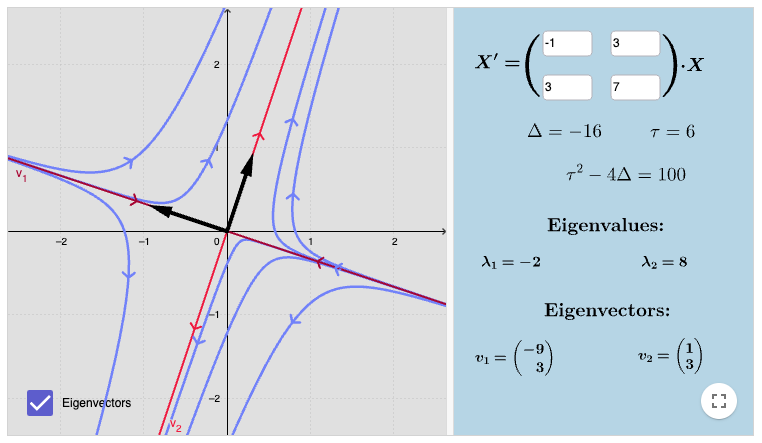
\includegraphics[width=5in]{Images/ImgPhasePlane1337.png}
        \end{center}         
    } 
    \else 
        \begin{center}
        \begin{tikzpicture}[scale=0.85]
        \draw[very thick, ->] (-3, 0) -- (3.25, 0);
        \draw[very thick, ->] (0, -3) -- (0, 3.25);
        \end{tikzpicture}
        \end{center}    
    \fi    

\end{parts}
\fi








\ifnum \Version=9
    \question[6] Consider the IVP $$\vec x \, ' = A\vec x, \quad A = \begin{pmatrix} -2&3\\3&-2 \end{pmatrix}, \quad \vec x = \begin{pmatrix} x(t)\\y(t)\end{pmatrix}, \quad \vec x(0) = \begin{pmatrix} 2\\2 \end{pmatrix}$$ The eigenvalues of $A$ are $\lambda_1 = -5$ and $\lambda_2 = 1$. 
    \begin{parts}
        \part Determine the eigenvectors of $A$. Please show your work. 
        
        \ifnum \Solutions=1 {\color{DarkBlue} 
        \textbf{Solutions:}
        For $\lambda_1$:
        \begin{align}
            A - \lambda_1 I = \begin{pmatrix} 3&3\\3&3\end{pmatrix} \ \Rightarrow \ v_1 = \begin{pmatrix} -1\\1 \end{pmatrix}
        \end{align}
        For $\lambda_2$:
        \begin{align}
            A - \lambda_2 I = \begin{pmatrix} -3&3\\3&-3\end{pmatrix} \ \Rightarrow \ v_2 = \begin{pmatrix} 1\\1 \end{pmatrix}
        \end{align}    
        } 
        \else 
            \vspace{6cm}   
        \fi        
        \part Use the given eigenvalues and the eigenvectors that you calculated in part (a) to solve the IVP.  
        
        \ifnum \Solutions=1 {\color{DarkBlue} 
        \textbf{Solutions:} the general solution to the DE is:
        $$\vec x = c_1 e^{-5t}\begin{pmatrix} -1\\1\end{pmatrix} + c_2e^{t} \begin{pmatrix} 1\\1\end{pmatrix}$$
        Use initial condition:
        \begin{align}
            \begin{pmatrix} 2\\2\end{pmatrix} &= c_1\begin{pmatrix}-1\\1 \end{pmatrix}+ c_2 \begin{pmatrix} 1\\1\end{pmatrix} \ \Rightarrow \ c_1 = 0, c_2 = 2 \ \Rightarrow \ 
            \vec x (t) = 2e^{t} \begin{pmatrix} 1\\1\end{pmatrix}
        \end{align}
        } 
        \else 
        \vspace{7cm}
    \fi
    \part Sketch the phase portrait of the system on the axes below. Please indicate the direction of motion on your solution curves and draw the eigenspaces corresponding to real eigenvalues (if any). Please also label your axes. 
    
    \ifnum \Solutions=1 {\color{DarkBlue} 
    \textbf{Solutions:}
        \begin{center}
        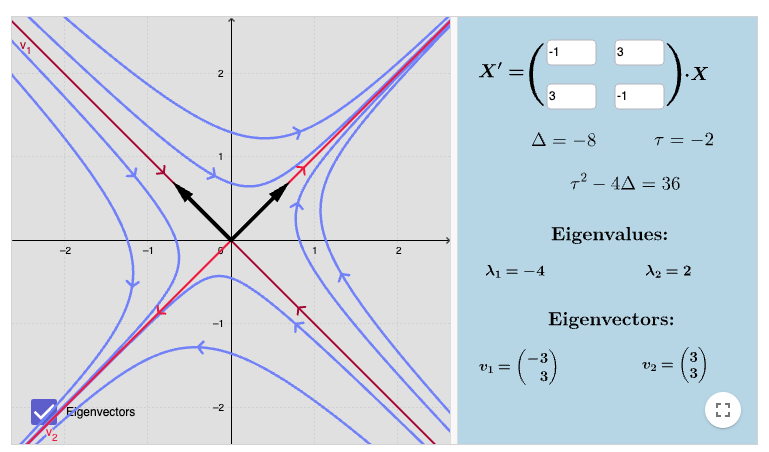
\includegraphics[width=5in]{Images/ImgPhasePlane1331.png}
        \end{center}         
    } 
    \else 
        \begin{center}
        \begin{tikzpicture}[scale=0.85]
        \draw[very thick, ->] (-3, 0) -- (3.25, 0);
        \draw[very thick, ->] (0, -3) -- (0, 3.25);
        \end{tikzpicture}
        \end{center}    
    \fi    

\end{parts}
\fi
    \ifnum \Version=1  
\question[8] Consider the differential equation $\displaystyle \frac{dy}{dt}= (y-2)(y-4k), \ k > 2$. The variable $y$ is a real function of $t$. Assume $y \in  \mathbb R$ and $t \ge 0$.
\fi
\ifnum \Version=2  
\question[8] Consider the differential equation $\displaystyle \frac{dy}{dt}= y^2-9$. The variable $y$ is a real function of $t$. Assume $y \in  \mathbb R$ and $t \ge 0$.
\fi 
\ifnum \Version=3
\question[8] Consider the differential equation $\displaystyle \frac{dy}{dt}= (y-1)(y+2)$. The variable $y$ is a real function of $t$. Assume $y \in  \mathbb R$ and $t \ge 0$.
\fi 
\ifnum \Version=4
\question[8] Consider the differential equation $\displaystyle \frac{dy}{dt}= y^2-4$. The variable $y$ is a real function of $t$. Assume $y \in  \mathbb R$ and $t \ge 0$.
\fi 
\ifnum \Version=5
\question[8] Consider the differential equation $\displaystyle \frac{dy}{dt}= (y+2)(y-3)$. The variable $y$ is a real function of $t$. Assume $y \in  \mathbb R$ and $t \ge 0$.
\fi 

\ifnum \Version<6
\begin{parts}
\part State the critical points of the differential equation.\vspace{1cm}
\part Draw the phase line, and determine whether the critical points (if any) are stable, semi-stable, or unstable.
\vspace{4cm}
\part Determine where $y$ is concave up and where $y$ is concave down for all $y \in \mathbb R$.  Show your work.
\vspace{7cm}
\part Use your results from parts A, B, and C to sketch several solution curves in the $ty$-plane for $y \in \mathbb R$ and $t \ge 0$. Clearly indicate the critical points and the points where the concavity changes. Please label your axes.     
\end{parts}
\fi


\ifnum \Version>5
\question[4] Consider the DE $\displaystyle \dydt = (y-4)(y-8)=y^2-12y+32$. Determine the values of $y$ where the solution curves are concave up and where the curves are concave down. Please show your work. 
\ifnum \Solutions=1 {\color{DarkBlue} 
    \text{Solutions:} Setting $y'=0$ we find that the equilibrium points are $y = 4, 6.$ And if $f(y) = y'$, then $$\dydtt = \dfdy \, \dydt$$ Also 
    $$\dfdy = \ddy\left(y^2-12y+32)\right) = 2y-12 = 2(y-6)$$
    So $df/dy = 0$ when $y=6$. There may be inflection points where either (or both) $df/dy$ and $dy/dt$ are zero. So there could be inflection points at $$y = 4, \ y = 8$$ A table will help determine concavity. When both derivatives have the same sign, the solutions are concave up, and when they have opposite signs the solutions are concave down. 
    \begin{center}            
        \renewcommand{\arraystretch}{1.4}
        \begin{tabular}{c|cccc} 
        $ y $ & $ (-\infty,4) $ & $(4,6)$ & $(6,8)$ & $(8,\infty)$  \\ \hline 
        $\displaystyle  dy/dt=(y-4)(y-8)$ & $+$ & $-$ & $-$ & $+$  \\ \hline
        $ \displaystyle df/dy = 2(y-6) $ & $-$ & $-$ & $+$ & $+$  \\[4pt] \hline
        $ \text{concavity} $ & \text{down} & \text{up} & \text{down} & \text{up} \\ \hline
        \end{tabular}
    \end{center}  
    So concave up on $y>8$ and $4<y<6$. Concave down on $y<4$, and $6<y<8$. 
} 
\else 
\fi
\fi 




        
\end{questions}

% SCRATCH
\ifnum \Solutions=0 \newpage 
    \begin{center}
        \textit{This page can be used for scratch work. }
    \end{center}
\fi
    % VERSION D
    \newpage 
    \renewcommand{\Version}{9} 
    % TEST SPECIFIC INFORMATION
% SAMPLE
\ifnum \Version=1 \renewcommand{\TestName}{Sample Test 1} \fi
% 2023 VERSIONS
\ifnum \Version=2 \renewcommand{\TestName}{Test 1 Version A} \fi
\ifnum \Version=3 \renewcommand{\TestName}{Test 1 Version B} \fi
\ifnum \Version=4 \renewcommand{\TestName}{Test 1 Version C} \fi
\ifnum \Version=5 \renewcommand{\TestName}{Test 1 Version D} \fi
% 2024 VERSIONS
\ifnum \Version=6 \renewcommand{\TestName}{Test 1 Version A} \fi
\ifnum \Version=7 \renewcommand{\TestName}{Test 1 Version B} \fi
\ifnum \Version=8 \renewcommand{\TestName}{Test 1 Version C} \fi
\ifnum \Version=9 \renewcommand{\TestName}{Test 1 Version D} \fi
\ifnum \Version=10 \renewcommand{\TestName}{Test 1 Make-Up} \fi

    % COLORED BOX FORMATTING
    % These boxes are used for definitions and theorems 
    % This code has to appear after begin{document}
    \tikzstyle{mybox} = [draw=black, fill=black!2, very thick, rectangle, rounded corners, inner sep=10pt, inner ysep=10pt]
    \tikzstyle{fancytitle} =[draw=black, very thick, fill=black!6, text=black, rounded corners]

    
% HEADERS AND FOOTERS
\pagestyle{headandfoot}
% \runningfooter{}{}{}
\runningfooter{}{}{\textit{Page \thepage \ of \pageref{LastPage}} }
\runningheader{\textit{Please write your last name: \framebox{\strut\hspace{5cm}} }}{}{\textit{\TestName} }
% \headheight 42pt % distance from top of page to top of header
% \headsep 12pt % space between header and top of body

\vspace*{-1cm}

\begin{center}
{\Large \TestName, \Course}
\end{center}
\renewcommand{\ID}{Please print your first name: \framebox{\strut\hspace{4.2cm}}, last name: \framebox{\strut\hspace{4.2cm}}, \\[2pt] and the remaining digits of your GTID:  \framebox{\strut $9$}\framebox{\strut $0$}\framebox{\strut\hspace{0.19cm}}\framebox{\strut\hspace{0.19cm}}\framebox{\strut\hspace{0.19cm}}\framebox{\strut\hspace{0.19cm}}\framebox{\strut\hspace{0.19cm}}\framebox{\strut\hspace{0.19cm}}\framebox{\strut\hspace{0.19cm}}.}

\ID

\begin{center}
    \setlength{\extrarowheight}{0.25cm}
    {\Large Helpful Formulas} \\
    \vspace{12pt}
    \textbf{Complex Solutions to 2D First Order Systems}
    \begin{align*}
        \lambda &= \alpha + i \beta, \ \beta \ne 0 , \ \vec v = \vec a + i \vec b \\
        \vec x_1 &= e^{\alpha t} (\vec a \cos \beta t - \vec b \sin \beta t), \quad 
        \vec x_{2} = e^{\alpha t} (\vec a \sin \beta t + \vec b \cos \beta t)
    \end{align*}
    \textbf{Repeated Eigenvalues in First Order 2D Systems}
    \begin{align*}
        (A-\lambda I) \vec w &= \vec v, \quad \vec w = t\vec v + \vec c
    \end{align*}    
\end{center}
    \begin{questions}


    \ifnum \Version=1  
\question[4] You do not need to show your work for this question. Consider the differential equation (DE) below.
$$\displaystyle t^2 \, \frac{d^2y}{dt^2} + \dydt = y^4$$
\begin{parts}
    \part Fill in the appropriate circle to indicate whether the DE is linear or non-linear
    \begin{itemize}
        \item[$\bigcirc$] The DE is linear.
        \item[$\bigcirc$] The DE is non-linear.
    \end{itemize}
    \part What is the order of the DE? \framebox{\strut\hspace{2cm}}
    \part Fill in the appropriate circle to indicate whether the DE is autonomous or non-autonomous. 
    \begin{itemize}        
        \item[$\bigcirc$] The DE is autonomous.
        \item[$\bigcirc$] The DE is non-autonomous.
    \end{itemize}    
    \part Is the DE is homogeneous or inhomogeneous? 
    \begin{itemize}        
        \item[$\bigcirc$] The DE is homogeneous.
        \item[$\bigcirc$] The DE is inhomogeneous.
    \end{itemize}        
\end{parts}
\fi 
\ifnum \Version=2
\question[4] You do not need to show your work for this question. Consider the differential equation below.
$$\displaystyle t^3 \, \frac{d^2y}{dt^2} + t\, \dydt + 2y^2 = \cos t$$
\begin{parts}
    \part Indicate whether the DE is homogeneous or inhomogeneous by filling in the appropriate circle. 
    \begin{itemize}        
        \item[$\bigcirc$] The DE is homogeneous.
        \item[$\bigcirc$] The DE is inhomogeneous.
    \end{itemize}     
    \part Fill in the appropriate circle to indicate whether the DE is linear or non-linear
    \begin{itemize}
        \item[$\bigcirc$] The DE is linear.
        \item[$\bigcirc$] The DE is non-linear.
    \end{itemize}
    \part Indicate whether the DE is autonomous or non-autonomous by filling in the appropriate circle. 
    \begin{itemize}        
        \item[$\bigcirc$] The DE is autonomous.
        \item[$\bigcirc$] The DE is non-autonomous.
    \end{itemize}       
    \part What is the order of the DE? \framebox{\strut\hspace{2cm}}
\end{parts}
\fi 

\ifnum \Version=3
\question[4] You do not need to show your work for this question. Consider the differential equation below.
$$\displaystyle 2 \frac{d^2y}{dt^2} + \dydt + 4y = \cos t$$
\begin{parts}
    \part Indicate whether the DE is autonomous or non-autonomous by filling in the appropriate circle. 
    \begin{itemize}        
        \item[$\bigcirc$] The DE is autonomous.
        \item[$\bigcirc$] The DE is non-autonomous.
    \end{itemize}       
    \part Indicate whether the DE is homogeneous or inhomogeneous by filling in the appropriate circle. 
    \begin{itemize}        
        \item[$\bigcirc$] The DE is homogeneous.
        \item[$\bigcirc$] The DE is inhomogeneous.
    \end{itemize}     
    \part Fill in the appropriate circle to indicate whether the DE is linear or non-linear
    \begin{itemize}
        \item[$\bigcirc$] The DE is linear.
        \item[$\bigcirc$] The DE is non-linear.
    \end{itemize}
    \part What is the order of the DE? \framebox{\strut\hspace{2cm}}
\end{parts}
\fi 

\ifnum \Version=4
\question[4] You do not need to show your work for this question. Consider the differential equation below.
$$\displaystyle 2 \frac{d^3y}{dt^3} + \dydt + 4y = t^4$$
\begin{parts}
    \part Indicate whether the DE is autonomous or non-autonomous by filling in the appropriate circle. 
    \begin{itemize}        
        \item[$\bigcirc$] The DE is autonomous.
        \item[$\bigcirc$] The DE is non-autonomous.
    \end{itemize}       
    \part What is the order of the DE? \framebox{\strut\hspace{2cm}} 
    \part Indicate whether the DE is homogeneous or inhomogeneous by filling in the appropriate circle. 
    \begin{itemize}        
        \item[$\bigcirc$] The DE is homogeneous.
        \item[$\bigcirc$] The DE is inhomogeneous.
    \end{itemize}     
    \part Fill in the appropriate circle to indicate whether the DE is linear or non-linear
    \begin{itemize}
        \item[$\bigcirc$] The DE is linear.
        \item[$\bigcirc$] The DE is non-linear.
    \end{itemize}
\end{parts}
\fi 

\ifnum \Version=5
\question[4] You do not need to show your work for this question. Consider the differential equation below.
$$\displaystyle 2 \dydt + 4y^2 = 0$$
\begin{parts}    
    \part What is the order of the DE? \framebox{\strut\hspace{2cm}} 
    \part Indicate whether the DE is homogeneous or inhomogeneous by filling in the appropriate circle. 
    \begin{itemize}        
        \item[$\bigcirc$] The DE is homogeneous.
        \item[$\bigcirc$] The DE is inhomogeneous.
    \end{itemize}     
    \part Fill in the appropriate circle to indicate whether the DE is linear or non-linear
    \begin{itemize}
        \item[$\bigcirc$] The DE is linear.
        \item[$\bigcirc$] The DE is non-linear.
    \end{itemize}
    \part Indicate whether the DE is autonomous or non-autonomous by filling in the appropriate circle. 
    \begin{itemize}        
        \item[$\bigcirc$] The DE is autonomous.
        \item[$\bigcirc$] The DE is non-autonomous.
    \end{itemize}       
\end{parts}
\fi 


\ifnum \Version=6
\question[4] You do not need to show your work for this question. Consider the differential equation below.
$$\displaystyle \dydtt + t^4 \, \frac{dy}{dt} + y = \cos(t)$$    
\begin{parts}
    \part Fill in the appropriate circle to indicate whether the DE is linear or non-linear.
    \begin{itemize}
        \item[$\bigcirc$] The DE is linear.
        \item[$\bigcirc$] The DE is non-linear.
    \end{itemize}
    \part Indicate whether the DE is autonomous or non-autonomous. 
    \begin{itemize}        
        \item[$\bigcirc$] The DE is autonomous.
        \item[$\bigcirc$] The DE is non-autonomous.
    \end{itemize}    
    \part Indicate whether the DE is homogeneous or non-homogeneous. 
    \begin{itemize}        
        \item[$\bigcirc$] The DE is homogeneous.
        \item[$\bigcirc$] The DE is non-homogeneous.
    \end{itemize}    
    \part What is the order of the DE? \framebox{\strut\hspace{4cm}}
    \vspace{2pt}   
    
\end{parts}
\ifnum \Solutions=1 {\color{DarkBlue} 
\textbf{Solutions:}
The DE can be classified as:
\begin{enumerate}
    \item \textbf{linear} because the coefficients are functions of $t$ only
    \item \textbf{not autonomous} because $t$ appears in the coefficients
    \item \textbf{not homogeneous} because of the $\cos t$ term
    \item \textbf{second order} because the highest degree derivative is 2    
\end{enumerate}
} 
\else 
\fi
\fi 




\ifnum \Version=7
\question[4] You do not need to show your work for this question. Consider the differential equation below.
$$\displaystyle \dydttt + t^4 \, \frac{dy}{dt} = y^2$$    
\begin{parts}
    \part Fill in the appropriate circle to indicate whether the DE is linear or non-linear.
    \begin{itemize}
        \item[$\bigcirc$] The DE is linear.
        \item[$\bigcirc$] The DE is non-linear.
    \end{itemize}
    \part Indicate whether the DE is autonomous or non-autonomous. 
    \begin{itemize}        
        \item[$\bigcirc$] The DE is autonomous.
        \item[$\bigcirc$] The DE is non-autonomous.
    \end{itemize}    
    \part Indicate whether the DE is homogeneous or non-homogeneous. 
    \begin{itemize}        
        \item[$\bigcirc$] The DE is homogeneous.
        \item[$\bigcirc$] The DE is non-homogeneous.
    \end{itemize}    
    \part What is the order of the DE? \framebox{\strut\hspace{4cm}}
    \vspace{2pt}   
    
\end{parts}
\ifnum \Solutions=1 {\color{DarkBlue} 
\textbf{Solutions:}
The DE can be classified as:
\begin{enumerate}
    \item \textbf{non-linear} because of the $y^2$ term
    \item \textbf{not autonomous} because $t$ appears in the coefficients
    \item \textbf{homogeneous} because there are no terms that are only functions of $t$
    \item \textbf{third order} because the highest degree derivative is 3  
\end{enumerate}
} 
\else 
\fi
\fi 




\ifnum \Version=8
\question[4] You do not need to show your work for this question. Consider the differential equation below.
$$\displaystyle \dydt + y^2 = t^3$$    
\begin{parts}
    \part Fill in the appropriate circle to indicate whether the DE is linear or non-linear.
    \begin{itemize}
        \item[$\bigcirc$] The DE is linear.
        \item[$\bigcirc$] The DE is non-linear.
    \end{itemize}
    \part Indicate whether the DE is autonomous or non-autonomous. 
    \begin{itemize}        
        \item[$\bigcirc$] The DE is autonomous.
        \item[$\bigcirc$] The DE is non-autonomous.
    \end{itemize}    
    \part Indicate whether the DE is homogeneous or non-homogeneous. 
    \begin{itemize}        
        \item[$\bigcirc$] The DE is homogeneous.
        \item[$\bigcirc$] The DE is non-homogeneous.
    \end{itemize}    
    \part What is the order of the DE? \framebox{\strut\hspace{4cm}}
    \vspace{2pt}   
    
\end{parts}
\ifnum \Solutions=1 {\color{DarkBlue} 
\textbf{Solutions:}
The DE can be classified as:
\begin{enumerate}
    \item \textbf{non-linear} because of the $y^2$ term
    \item \textbf{not autonomous} because $t$ appears in the DE
    \item \textbf{not homogeneous} because there are terms that are only functions of $t$
    \item \textbf{first order} because the highest degree derivative is 1
\end{enumerate}
} 
\else 
\fi
\fi 





\ifnum \Version=9
\question[4] You do not need to show your work for this question. Consider the differential equation below.
$$\displaystyle \dydtt + \dydt + t^3y = 0$$    
\begin{parts}
    \part Fill in the appropriate circle to indicate whether the DE is linear or non-linear.
    \begin{itemize}
        \item[$\bigcirc$] The DE is linear.
        \item[$\bigcirc$] The DE is non-linear.
    \end{itemize}
    \part Indicate whether the DE is autonomous or non-autonomous. 
    \begin{itemize}        
        \item[$\bigcirc$] The DE is autonomous.
        \item[$\bigcirc$] The DE is non-autonomous.
    \end{itemize}    
    \part Indicate whether the DE is homogeneous or non-homogeneous. 
    \begin{itemize}        
        \item[$\bigcirc$] The DE is homogeneous.
        \item[$\bigcirc$] The DE is non-homogeneous.
    \end{itemize}    
    \part What is the order of the DE? \framebox{\strut\hspace{4cm}}
    \vspace{2pt}   
    
\end{parts}
\ifnum \Solutions=1 {\color{DarkBlue} 
\textbf{Solutions:}
The DE can be classified as:
\begin{enumerate}
    \item \textbf{linear} because the coefficients are only functions of $t$
    \item \textbf{not autonomous} because $t$ appears in the DE
    \item \textbf{ homogeneous} because there are no terms that are only functions of $t$
    \item \textbf{second order} because the highest degree derivative is 2
\end{enumerate}
} 
\else 
\fi
\fi 
    \ifnum \Version=1  
\question[2] Consider the autonomous differential equation $\displaystyle \frac{dy}{dt}= (y-1)(y-k^2)$.  Assume $k$ can be any real number. Draw the bifurcation diagram on the axes below. That is, plot the location of the critical points versus $k$. Please label your axes.
        \begin{center}
        \begin{tikzpicture}[scale=0.85]
        \draw[help lines] (-2.5,-2.5) grid (2.5, 2.5);
        \draw[very thick, ->] (-3, 0) -- (3.25, 0);
        \draw[very thick, ->] (0, -3) -- (0, 3.25);
        \node[overlay, left] at (-0.2, 1) {$1$};
        \node[overlay, left] at (-0.2, 2) {$2$};
        \node[overlay, below] at (-0.5, -0.2) {$0$};
        \node[overlay, below] at (1, -0.2) {$1$};
        \node[overlay, below] at (2, -0.2) {$2$};
        \end{tikzpicture}
        \end{center}
\fi

\ifnum \Version=2
\question[2] Consider the autonomous differential equation $\displaystyle \frac{dy}{dt}= (y-k)(y+1-k^2)$.  Assume $k$ can be any real number. Draw the bifurcation diagram on the axes below. That is, plot the location of the critical points versus $k$. Please label your axes.
        \begin{center}
        \begin{tikzpicture}[scale=0.85]
        \draw[help lines] (-2.5,-2.5) grid (2.5, 2.5);
        \draw[very thick, ->] (-3, 0) -- (3.25, 0);
        \draw[very thick, ->] (0, -3) -- (0, 3.25);
        \node[overlay, left] at (-0.2, 1) {$1$};
        \node[overlay, left] at (-0.2, 2) {$2$};
        \node[overlay, below] at (-0.5, -0.2) {$0$};
        \node[overlay, below] at (1, -0.2) {$1$};
        \node[overlay, below] at (2, -0.2) {$2$};
        \end{tikzpicture}
        \end{center}
\fi

\ifnum \Version=3
    \question[2] You do not need to show your work for this question. Consider the differential equation 
    \begin{align*}
        t^2y'' - 4ty' - 2y = 12
    \end{align*}
    The DE can be expressed in the form $\vec x\, ' = A\vec x + \vec g$, where 
    \begin{align*}
     A = \left( \hbox to 2cm{\vbox to 0.85cm{}} \right), \quad \vec g = \left( \hbox to 1.2cm{\vbox to 0.85cm{}} \right)
    \end{align*}
    Fill in the missing entries in the above to define $A$ and $\vec g$. 
\fi

\ifnum \Version=4
\question[2] Consider the autonomous differential equation $\displaystyle \frac{dy}{dt}= (y+k)(y^2-k)$.  Assume $k\ge0$. Draw the bifurcation diagram on the axes below. That is, plot the location of the critical points versus $k$. Please label your axes.
        \begin{center}
        \begin{tikzpicture}[scale=0.85]
        \draw[help lines] (-2.5,-2.5) grid (2.5, 2.5);
        \draw[very thick, ->] (-3, 0) -- (3.25, 0);
        \draw[very thick, ->] (0, -3) -- (0, 3.25);
        \node[overlay, left] at (-0.2, 1) {$1$};
        \node[overlay, left] at (-0.2, 2) {$2$};
        \node[overlay, below] at (-0.5, -0.2) {$0$};
        \node[overlay, below] at (1, -0.2) {$1$};
        \node[overlay, below] at (2, -0.2) {$2$};
        \end{tikzpicture}
        \end{center}
\fi

\ifnum \Version=5
    \question[2] You do not need to show your work for this question. Consider the differential equation 
    \begin{align*}
        4y'' - t^2y' - 2ty = 12\cos(t)
    \end{align*}
    The DE can be expressed in the form $\vec x\, ' = A\vec x + \vec g$, where 
    \begin{align*}
     A = \left( \hbox to 2cm{\vbox to 0.85cm{}} \right), \quad \vec g = \left( \hbox to 1.2cm{\vbox to 0.85cm{}} \right)
    \end{align*}
    Fill in the missing entries in the above to define $A$ and $\vec g$. 
\fi




\ifnum \Version=6
\question[1] You do not need to show your work for this question. Consider the IVP below.
$$\displaystyle y' = \sqrt{4-t^2+y}, \ y(1) = 2$$   
Using the theorems we covered in lecture, fill in all of the appropriate circles below to indicate the intervals over which there must contain a unique solution to the IVP. 
\begin{itemize}
    \item[$\bigcirc$] $y \ge 4-t^2$
    \item[$\bigcirc$] $y \le 4-t^2$
    \item[$\bigcirc$] $y \le t^2-4$
    \item[$\bigcirc$] $y \ge t^2-4$
    \item[$\bigcirc$] none of the above
\end{itemize}
\ifnum \Solutions=1 {\color{DarkBlue} 
\textbf{Solutions:} the relevant theorem is below. 

    \begin{center}\begin{tikzpicture} \node [mybox](box){\begin{minipage}{0.95\textwidth} \vspace{4pt}

    If $f$ and $\frac{\partial f}{\partial y}$ are continuous over $\alpha < t < \beta$, and $\gamma < y < \delta$, which contains the point $(t_0,y_0)$, then there is a unique solution to the IVP $$y' = f(t,y), \quad y(t_0) = y_0$$ on an interval contained in $\alpha < t < \beta$. 
    
    \end{minipage}}; \node[fancytitle, rounded corners, thick, inner sep = 4pt, right=10pt] at (box.north west) {Theorem 2.4.2: Existence and Uniqueness of 1st Order Nonlinear IVP};
    \end{tikzpicture}\end{center}
    
    Taking the partial derivative with respect to $y$:
\begin{align}
    \frac{\partial f}{\partial y} &= \frac{1}{\sqrt{4-t^2+y}}\\
\end{align}
The relevant functions are 
\begin{align}
    f(t,y) &= \sqrt{4-t^2+y} \\
    \frac{\partial f}{\partial y} &= \frac{1}{\sqrt{4-t^2+y}}
\end{align}
They are real and continuous over $$4-t^2+y > 0$$ and this interval also contains $t_0 = 0$ and $y(t_0)$. So the interval over which there must contain a unique solution is $$y > t^2-4$$ 
} 
\else 
\fi
\fi 




\ifnum \Version=7
\question[1] You do not need to show your work for this question. Consider the IVP below.
$$\displaystyle (t+3)y' + \sqrt{4-t^2}\,y = t^4, \ y(1) = 9$$   
Using the theorems we covered in lecture, fill in all of the appropriate circles below to indicate the intervals over which there must contain a unique solution to the IVP. 
\begin{itemize}
    \item[$\bigcirc$] $-3 < t \le 2$
    \item[$\bigcirc$] $-2 \le t \le 2$
    \item[$\bigcirc$] $-2 \le t \le 3$    
    \item[$\bigcirc$] $-\infty \le t < -3$
    \item[$\bigcirc$] none of the above
\end{itemize}
\ifnum \Solutions=1 {\color{DarkBlue} 
\textbf{Solutions:} convert to standard form:
\begin{align}
    y' + \frac{\sqrt{4-t^2}}{t+3}\,y = \frac{t^4}{t+3}
\end{align}
The coefficients are real and continuous over $$-2\le t \le 2$$ and this interval also contains $t_0 = 1$. So the interval over which there must contain a unique solution is $-2\le t \le 2$. 
} 
\else 
\fi
\fi 



\ifnum \Version=8
\question[1] You do not need to show your work for this question. Consider the IVP below.
$$\displaystyle y' = \sqrt{4-t^2-y}, \ y(0) = 2$$   
Using the theorems we covered in lecture, fill in all of the appropriate circles below to indicate the intervals over which there must contain a unique solution to the IVP. 
\begin{itemize}
    \item[$\bigcirc$] $y \ge 4-t^2$
    \item[$\bigcirc$] $y \le 4-t^2$
    \item[$\bigcirc$] $y \le t^2-4$
    \item[$\bigcirc$] $y \ge t^2-4$
    \item[$\bigcirc$] none of the above
\end{itemize}
\ifnum \Solutions=1 {\color{DarkBlue} 
\textbf{Solutions:} partial derivative with respect to $y$:
\begin{align}
    \frac{\partial f}{\partial y} &= \frac{-1}{\sqrt{4-t^2-y}}
\end{align}
The coefficients are real and continuous over $$4-t^2-y\ge 0$$ and this interval also contains $t_0 = 0$ and $y(t_0)$. So the interval over which there must contain a unique solution is $y \le 4-t^2$. 
} 
\else 
\fi
\fi 



\ifnum \Version=9
\question[1] You do not need to show your work for this question. Consider the IVP below.
$$\displaystyle y' = \sqrt{4-t^2+y}, \ y(0) = 2$$   
Using the theorems we covered in lecture, fill in all of the appropriate circles below to indicate the intervals over which there must contain a unique solution to the IVP. 
\begin{itemize}
    \item[$\bigcirc$] $y \ge 4-t^2$
    \item[$\bigcirc$] $y \le 4-t^2$
    \item[$\bigcirc$] $y \le t^2-4$
    \item[$\bigcirc$] $y \ge t^2-4$
    \item[$\bigcirc$] none of the above
\end{itemize}
\ifnum \Solutions=1 {\color{DarkBlue} 
\textbf{Solutions:} partial derivative with respect to $y$:
\begin{align}
    \frac{\partial f}{\partial y} &= \frac{1}{\sqrt{4-t^2+y}}\\
\end{align}
The coefficients are real and continuous over $$4-t^2+y\ge 0$$ and this interval also contains $t_0 = 0$ and $y(t_0)$. So the interval over which there must contain a unique solution is $y \ge t^2-4$. 
} 
\else 
\fi
\fi 




    \ifnum \Version=6
\question[3] Consider the system $$\vec x \, ' = A\vec x, \quad A = \begin{pmatrix} -3&-4\\1&-1 \end{pmatrix}, \quad \vec x = \begin{pmatrix} x(t)\\y(t)\end{pmatrix} $$ The eigenvalues of $A$ are $\lambda = -2\pm i\sqrt 3$. Sketch the phase portrait of the system. Sketch at least two solution curves. Please indicate the direction of motion on your solution curves. Don't forget to label your axes.   

\ifnum \Solutions=1 {\color{DarkBlue} 
\textbf{Solutions:} solution curves should \textbf{spiral towards} the origin and rotate \textbf{counter clockwise}. Axes should be labelled. Ok to only draw only two solution curves. 
    \begin{center}
    \begin{tikzpicture}[scale=0.75]
      \draw[ultra thick,->,>=latex] (-2.5,0)--(2.5,0) node[below] {x};
      \draw[ultra thick,->,>=latex] (0,-2.5)--(0,2.5) node[left] {y};      
      \draw[domain=0:6,ultra thick,samples=20,DarkRed] plot ({cos(deg(\x))*2*exp(-\x/3},{sin(deg(\x))*2*exp(-\x/3});
      \draw[domain=0:1,->,ultra thick,samples=20,DarkRed] plot ({cos(deg(\x))*2*exp(-\x/3},{sin(deg(\x))*2*exp(-\x/3});
      \draw[domain=0:6,ultra thick,samples=20,DarkRed] plot ({.75*cos(deg(\x))*2*exp(-\x/3},{.75*sin(deg(\x))*2*exp(-\x/3});
      \draw[domain=0:1,->,ultra thick,samples=20,DarkRed] plot ({.75*cos(deg(\x))*2*exp(-\x/3},{.75*sin(deg(\x))*2*exp(-\x/3});
    \end{tikzpicture}
    \end{center} 
} 
\else 
    \begin{center}
    \begin{tikzpicture}[scale=0.75]
      \draw[ultra thick,->,>=latex] (-2.5,0)--(2.5,0) node[below] {};
      \draw[ultra thick,->,>=latex] (0,-2.5)--(0,2.5) node[left] {};         
    \end{tikzpicture}
    \end{center} 
\fi
\fi


\ifnum \Version=7
\question[3] Consider the system $$\vec x \, ' = A\vec x, \quad A = \begin{pmatrix} 3&2\\-5&1 \end{pmatrix}, \quad \vec x = \begin{pmatrix} x(t)\\y(t)\end{pmatrix} $$ The eigenvalues of $A$ are $\lambda = 2\pm  3i$. Sketch the phase portrait of the system. Sketch at least two solution curves. Please indicate the direction of motion on your solution curves. Don't forget to label your axes.   

\ifnum \Solutions=1 {\color{DarkBlue} 
\textbf{Solutions:} solution curves should \textbf{spiral away} from the origin and rotate \textbf{clockwise}. Axes should be labelled. Ok to only draw only two solution curves. 
\begin{center}
    \begin{tikzpicture}[scale=0.75]
      \draw[ultra thick,->,>=latex] (-2.5,0)--(2.5,0) node[below] {x};
      \draw[ultra thick,->,>=latex] (0,-2.5)--(0,2.5) node[left] {y};      
      \draw[domain=0:8,ultra thick,samples=30,DarkRed] plot ({cos(deg(\x))*0.12*exp(\x/3)},{-sin(deg(\x))*0.12*exp(\x/3)});
      \draw[domain=0:6,->,ultra thick,samples=30,DarkRed] plot ({cos(deg(\x))*0.12*exp(\x/3)},{-sin(deg(\x))*0.12*exp(\x/3)});
      \draw[domain=0:8,ultra thick,samples=30,DarkRed] plot ({cos(deg(\x))*0.2*exp(\x/3)},{-sin(deg(\x))*0.2*exp(\x/3)});
      \draw[domain=0:6,->,ultra thick,samples=30,DarkRed] plot ({cos(deg(\x))*0.2*exp(\x/3)},{-sin(deg(\x))*0.2*exp(\x/3)});      
    \end{tikzpicture}
\end{center} 
} 
\else 
\begin{center}
    \begin{tikzpicture}[scale=0.75]
      \draw[ultra thick,->,>=latex] (-2.5,0)--(2.5,0) node[below] {};
      \draw[ultra thick,->,>=latex] (0,-2.5)--(0,2.5) node[left] {};         
    \end{tikzpicture}
\end{center} 
\fi
\fi






\ifnum \Version=8
\question[3] Consider the system $$\vec x \, ' = A\vec x, \quad A = \begin{pmatrix} -3&-4\\1&-1 \end{pmatrix}, \quad \vec x = \begin{pmatrix} x(t)\\y(t)\end{pmatrix} $$ The eigenvalues of $A$ are $\lambda = -2\pm i\sqrt 3$. Sketch the phase portrait of the system. Sketch at least two solution curves. Please indicate the direction of motion on your solution curves. Don't forget to label your axes.   

\ifnum \Solutions=1 {\color{DarkBlue} 
\textbf{Solutions:} solution curves should spiral towards center and rotate counter clockwise. Axes should be labelled. Ok to only draw only two solution curves. 
    \begin{center}
    \begin{tikzpicture}[scale=0.75]
      \draw[ultra thick,->,>=latex] (-2.5,0)--(2.5,0) node[below] {x};
      \draw[ultra thick,->,>=latex] (0,-2.5)--(0,2.5) node[left] {y};      
      \draw[domain=0:6,ultra thick,samples=20,DarkRed] plot ({cos(deg(\x))*2*exp(-\x/3},{sin(deg(\x))*2*exp(-\x/3});
      \draw[domain=0:1,->,ultra thick,samples=20,DarkRed] plot ({cos(deg(\x))*2*exp(-\x/3},{sin(deg(\x))*2*exp(-\x/3});
      \draw[domain=0:6,ultra thick,samples=20,DarkRed] plot ({.75*cos(deg(\x))*2*exp(-\x/3},{.75*sin(deg(\x))*2*exp(-\x/3});
      \draw[domain=0:1,->,ultra thick,samples=20,DarkRed] plot ({.75*cos(deg(\x))*2*exp(-\x/3},{.75*sin(deg(\x))*2*exp(-\x/3});
    \end{tikzpicture}
    \end{center} 
} 
\else 
    \begin{center}
    \begin{tikzpicture}[scale=0.75]
      \draw[ultra thick,->,>=latex] (-2.5,0)--(2.5,0) node[below] {};
      \draw[ultra thick,->,>=latex] (0,-2.5)--(0,2.5) node[left] {};         
    \end{tikzpicture}
    \end{center} 
\fi
\fi




\ifnum \Version=9
\question[3] Consider the system $$\vec x \, ' = A\vec x, \quad A = \begin{pmatrix} 1&-4\\1&3 \end{pmatrix}, \quad \vec x = \begin{pmatrix} x(t)\\y(t)\end{pmatrix} $$ The eigenvalues of $A$ are $\lambda = 2\pm i\sqrt 3$. Sketch the phase portrait of the system. Sketch at least two solution curves. Please indicate the direction of motion on your solution curves. Don't forget to label your axes.   

\ifnum \Solutions=1 {\color{DarkBlue} 
\textbf{Solutions:} solution curves should spiral away from the origin and rotate counter clockwise. Axes should be labelled. Ok to only draw only two solution curves. 
    \begin{center}
    \begin{tikzpicture}[scale=0.75]
      \draw[ultra thick,->,>=latex] (-2.5,0)--(2.5,0) node[below] {x};
      \draw[ultra thick,->,>=latex] (0,-2.5)--(0,2.5) node[left] {y};      
      \draw[domain=0:8,ultra thick,samples=30,DarkRed] plot ({cos(deg(\x))*0.12*exp(\x/3)},{sin(deg(\x))*0.12*exp(\x/3)});
      \draw[domain=0:4,->,ultra thick,samples=30,DarkRed] plot ({cos(deg(\x))*0.12*exp(\x/3)},{sin(deg(\x))*0.12*exp(\x/3)});
      \draw[domain=0:8,ultra thick,samples=30,DarkRed] plot ({cos(deg(\x))*0.2*exp(\x/3)},{sin(deg(\x))*0.2*exp(\x/3)});
      \draw[domain=0:4,->,ultra thick,samples=30,DarkRed] plot ({cos(deg(\x))*0.2*exp(\x/3)},{sin(deg(\x))*0.2*exp(\x/3)});      
    \end{tikzpicture}
    \end{center} 
} 
\else 
    \begin{center}
    \begin{tikzpicture}[scale=0.75]
      \draw[ultra thick,->,>=latex] (-2.5,0)--(2.5,0) node[below] {};
      \draw[ultra thick,->,>=latex] (0,-2.5)--(0,2.5) node[left] {};         
    \end{tikzpicture}
    \end{center} 
\fi
\fi



    
\ifnum \Version>5
\question[3] A tank originally contains 50 L of water with 6 kg of salt. Water containing $\frac{1}{20}$ kg of salt per litre is entering at a rate of 4 L/hour, and the well-stirred solution in the tank is leaving at 1 L/hour. 

\begin{parts}
    \part Write down an IVP for $V(t)$, which is the amount of fluid in the tank at time $t$. You do not need to solve your IVP. 
    
    \ifnum \Solutions=1 {\color{DarkBlue} 
        The volume of fluid in the tank is
        $$V = 50 + 3t$$
        By differentiating, the IVP for $V(t)$ is
        $$\frac{dV}{dt} = 3, \quad V(0) = 50$$
        }
    \else
    \vspace{6cm}
    \fi
    
    \part Write down an IVP for $Q(t)$, for the amount of salt in the tank. You do not need to solve the IVP. 
    
    \ifnum \Solutions=1 {\color{DarkBlue} 
        The DE is
        \begin{align}
            \frac{dQ}{dt} &= \left( \text{rate salt coming in} \right) - \left( \text{rate of salt going out} \right) \\
            \frac{dQ}{dt} &= 4\cdot \frac{1}{20} - \frac{Q}{V}
        \end{align}
        The IVP is
        \begin{align}
            \frac{dQ}{dt} &= \frac{1}{5} - \frac{Q}{50+3t}, \quad Q(0) = 6
        \end{align}        
        }
        \fi
    \fi
    
\end{parts}


        

    \newpage        
    \newpage 
\ifnum \Version=1  
\question[4] Solve the initial value problem and solve for $y$ to obtain an explicit expression for $y$ in terms of $t$. Please show your work.
$$\displaystyle t\,\frac{dy}{dt} = \frac{\cos(t)}{t^2} - 3y, \quad y(\pi) = 2, \quad t > 0$$.
\fi

\ifnum \Version=2
\question[4] Solve the initial value problem and solve for $y$ to obtain an explicit expression for $y$ in terms of $t$. Please show your work.
$$\displaystyle \frac{dy}{dt} = 12e^{3t}e^{-2y}, \quad y(0) = 2, \quad t \ge 0$$.
\fi

\ifnum \Version=3
\question[4] Solve the initial value problem and solve for $y$ to obtain an explicit expression for $y$ in terms of $t$. Please show your work.
$$\displaystyle t\,\frac{dy}{dt} + 3y =  36 t^{-2}e^{-t}, \ y(1) = 0, \quad t > 0$$.
\fi   

\ifnum \Version=4
\question[4] Solve the initial value problem and solve for $y$ to obtain an expression for $y$ in terms of $t$. Please show your work.
$$\displaystyle \frac{dy}{dt} = \frac{16e^{2t}}{y}, \quad y(1) = 2, \quad t > 0$$.
\fi

\ifnum \Version=5
\question[4] Solve the initial value problem and solve for $y$ to obtain an explicit expression for $y$ in terms of $t$. Please show your work.
$$\displaystyle t\,\frac{dy}{dt} + 2y =  36 t^{-1}e^{t}, \ y(1) = 2e, \quad t > 0$$.
\fi   



\ifnum \Version=6
\question[4] 
Solve the initial value problem and solve for $y$ to obtain an explicit expression for $y$ in terms of $t$. Please show your work.
$$\displaystyle t\,\frac{dy}{dt} + 4y =  24 t^{-3}e^{2t}, \ y(1) = 2, \quad t > 0$$.

\ifnum \Solutions=1 {\color{DarkBlue} 
\textbf{Solutions:}
To solve the differential equation \( t y' + 4 y = 24 t^{-3} e^{2t} \) with the initial condition \( y(1) = 2 \), we can follow these steps.
\begin{enumerate}
    \item Rewrite the DE in standard form:
   \[ y' + \frac{4}{t} y = 24 t^{-4} e^{2t} \]
   \item Integrating factor:
   \[ \mu(t) = e^{\int \frac{4}{t} \, dt} = e^{4 \ln |t|} = t^4 \]
   \item Multiply both sides of the differential equation by the integrating factor:
   \begin{align*}
       t^4 y' + 4 t^3 y &= 24 e^{2t} \\
       \frac{d}{dt} (t^4 y) &= 24 e^{2t}
   \end{align*} 
   \item Integrate both sides with respect to \( t \) and solve for $y$:
   \begin{align}
       t^4 y &= \int 24 e^{2t} \, dt + C \\
       t^4 y &= 12 e^{2t} + C \\
        y &= \frac{12 e^{2t} + C}{t^4} 
   \end{align} 
   \item Apply the initial condition \( y(1) = 2 \):
   \[ 2 = \frac{12 e^{2 \cdot 1} + C}{1^4} \]
   \[ 2 = 12 e^2 + C \]
   \[ C = 2 - 12 e^2 \]
   \item Substitute \( C \) back into the solution:
   \[ y = \frac{12 e^{2t} + 2 - 12 e^2}{t^4} \]
\end{enumerate}
} 
\else 
\newpage
\fi
\fi   





\ifnum \Version=7
\question[4] 
Solve the initial value problem and solve for $y$ to obtain an explicit expression for $y$ in terms of $t$. Please show your work.
$$\displaystyle t\,\frac{dy}{dt} + 5y =  20 t^{-4}e^{2t}, \ y(1) = e^2, \quad t > 0$$.

\ifnum \Solutions=1 {\color{DarkBlue} 
\textbf{Solutions:}
To solve the differential equation \( t y' + 5 y = 20 t^{-3} e^{2t} \) with the initial condition \( y(1) = 2 \), we can follow these steps.
\begin{enumerate}
    \item Rewrite the DE in standard form:
   \[ y' + \frac{5}{t} y = 20 t^{-4} e^{2t} \]
   \item Integrating factor:
   \[ \mu(t) = e^{\int \frac{5}{t} \, dt} = e^{5 \ln |t|} = t^5 \]
   \item Multiply both sides of the differential equation by the integrating factor:
   \begin{align*}
       t^5 y' + 5 t^4 y &= 20 e^{2t} \\
       \frac{d}{dt} (t^5 y) &= 20 e^{2t}
   \end{align*} 
   \item Integrate both sides with respect to \( t \) and solve for $y$:
   \begin{align}
       t^5 y &= \int 20 e^{2t} \, dt + C \\
       t^5 y &= 10 e^{2t} + C \\
        y &= \frac{10 e^{2t} + C}{t^5} 
   \end{align} 
   \item Apply the initial condition \( y(1) = e^2 \):
   \[ e^2 = \frac{10 e^{2 \cdot 1} + C}{1^5} \]
   \[ e^2 = 10 e^2 + C \]
   \[ C = - 9 e^2 \]
   \item Substitute \( C \) back into the solution:
   \[ y = \frac{10 e^{2t} - 9 e^2}{t^5} \]
\end{enumerate}
} 
\else 
\newpage
\fi
\fi   






\ifnum \Version=8
\question[4] 
Solve the initial value problem and solve for $y$ to obtain an explicit expression for $y$ in terms of $t$. Please show your work.
$$\displaystyle t\,\frac{dy}{dt} + 6y =  24 t^{-5}e^{4t}, \ y(1) = 8e^4, \quad t > 0$$.

\ifnum \Solutions=1 {\color{DarkBlue} 
\textbf{Solutions:}
To solve the DE with the given initial condition we can follow these steps.
\begin{enumerate}
    \item Rewrite the DE in standard form:
   \[ y' + \frac{6}{t} y = 24 t^{-6} e^{4t} \]
   \item Integrating factor:
   \[ \mu(t) = e^{\int \frac{6}{t} \, dt} = e^{6 \ln |t|} = t^6 \]
   \item Multiply both sides of the differential equation by the integrating factor:
   \begin{align*}
       t^6 y' + 6 t^5 y &= 24 e^{4t} \\
       \frac{d}{dt} (t^6 y) &= 24 e^{4t}
   \end{align*} 
   \item Integrate both sides with respect to \( t \) and solve for $y$:
   \begin{align}
       t^6 y &= \int 24 e^{4t} \, dt + C \\
       t^6 y &= 6 e^{4t} + C \\
        y &= \frac{6 e^{4t} + C}{t^6} 
   \end{align} 
   \item Apply the initial condition:
   \[ 8e^4 = \frac{6 e^{4 \cdot 1} + C}{1^5} \]
   \[ 8e^4 = 6 e^4 + C \]
   \[ C = 2 e^4 \]
   \item Substitute \( C \) back into the solution:
   \[ y = \frac{6 e^{4t} +2 e^4}{t^6} \]
\end{enumerate}
} 
\else 
\newpage
\fi
\fi   



\ifnum \Version=9
\question[4] 
Solve the initial value problem and solve for $y$ to obtain an explicit expression for $y$ in terms of $t$. Please show your work.
$$\displaystyle t\,\frac{dy}{dt} + 5y =  20 t^{-4}e^{2t}, \ y(1) = e^2, \quad t > 0$$.

\ifnum \Solutions=1 {\color{DarkBlue} 
\textbf{Solutions:}
To solve the differential equation \( t y' + 5 y = 20 t^{-3} e^{2t} \) with the initial condition \( y(1) = 2 \), we can follow these steps.
\begin{enumerate}
    \item Rewrite the DE in standard form:
   \[ y' + \frac{5}{t} y = 20 t^{-4} e^{2t} \]
   \item Integrating factor:
   \[ \mu(t) = e^{\int \frac{5}{t} \, dt} = e^{5 \ln |t|} = t^5 \]
   \item Multiply both sides of the differential equation by the integrating factor:
   \begin{align*}
       t^5 y' + 5 t^4 y &= 20 e^{2t} \\
       \frac{d}{dt} (t^5 y) &= 20 e^{2t}
   \end{align*} 
   \item Integrate both sides with respect to \( t \) and solve for $y$:
   \begin{align}
       t^5 y &= \int 20 e^{2t} \, dt + C \\
       t^5 y &= 10 e^{2t} + C \\
        y &= \frac{10 e^{2t} + C}{t^5} 
   \end{align} 
   \item Apply the initial condition \( y(1) = e^2 \):
   \[ e^2 = \frac{10 e^{2 \cdot 1} + C}{1^5} \]
   \[ e^2 = 10 e^2 + C \]
   \[ C = - 9 e^2 \]
   \item Substitute \( C \) back into the solution:
   \[ y = \frac{10 e^{2t} - 9 e^2}{t^5} \]
\end{enumerate}
} 
\else 
\newpage
\fi
\fi   
        
    \newpage 

\ifnum \Version=1  
\question[7] Consider the system $$\vec x \, ' = A\vec x, \quad A = \begin{pmatrix} 0&3\\5&2 \end{pmatrix}, \quad \vec x = \begin{pmatrix} x(t)\\y(t)\end{pmatrix} $$.
\begin{parts}
    \part Determine the eigenvalues of $A$. Please show your work. \vspace{5cm}
    \part Determine the eigenvectors of $A$. Please show your work. \vspace{7cm}
    \part Sketch the phase portrait of the system on the axes below. Please indicate the direction of motion on your solution curves and draw the eigenspaces corresponding to real eigenvalues (if any). Please also label your axes. 
    \begin{center}
    \begin{tikzpicture}[scale=0.85]
    \draw[very thick, ->] (-3, 0) -- (3.25, 0);
    \draw[very thick, ->] (0, -3) -- (0, 3.25);
    \end{tikzpicture}
    \end{center}
\end{parts}
\fi

\ifnum \Version=2
\question[7] Consider the system $$\vec x \, ' = A\vec x, \quad A = \begin{pmatrix} 4&3\\3&-4 \end{pmatrix}, \quad \vec x = \begin{pmatrix} x(t)\\y(t)\end{pmatrix} $$.
\begin{parts}
    \part Determine the eigenvalues of $A$. Please show your work. \vspace{5cm}
    \part Determine the eigenvectors of $A$. Please show your work. \vspace{7cm}
    \part Sketch the phase portrait of the system on the axes below. Please indicate the direction of motion on your solution curves and draw the eigenspaces corresponding to real eigenvalues (if any). Please also label your axes. 
    \begin{center}
    \begin{tikzpicture}[scale=0.85]
    \draw[very thick, ->] (-3, 0) -- (3.25, 0);
    \draw[very thick, ->] (0, -3) -- (0, 3.25);
    \end{tikzpicture}
    \end{center}
\end{parts}
\fi

\ifnum \Version=3
\question[7] Consider the system $$\vec x \, ' = A\vec x, \quad A = \begin{pmatrix} 5&4\\-3&-3 \end{pmatrix}, \quad \vec x = \begin{pmatrix} x(t)\\y(t)\end{pmatrix} $$.
\begin{parts}
    \part Determine the eigenvalues of $A$. Please show your work. \vspace{5cm}
    \part Determine the eigenvectors of $A$. Please show your work. \vspace{7cm}
    \part Sketch the phase portrait of the system on the axes below. Please indicate the direction of motion on your solution curves and draw the eigenspaces corresponding to real eigenvalues (if any). Please also label your axes. 
    \begin{center}
    \begin{tikzpicture}[scale=0.85]
    \draw[very thick, ->] (-3, 0) -- (3.25, 0);
    \draw[very thick, ->] (0, -3) -- (0, 3.25);
    \end{tikzpicture}
    \end{center}
\end{parts}
\fi

\ifnum \Version=4
\question[7] Consider the system $$\vec x \, ' = A\vec x, \quad A = \begin{pmatrix} 3&4\\-3&-5 \end{pmatrix}, \quad \vec x = \begin{pmatrix} x(t)\\y(t)\end{pmatrix} $$.
\begin{parts}
    \part Determine the eigenvalues of $A$. Please show your work. \vspace{5cm}
    \part Determine the eigenvectors of $A$. Please show your work. \vspace{7cm}
    \part Sketch the phase portrait of the system on the axes below. Please indicate the direction of motion on your solution curves and draw the eigenspaces corresponding to real eigenvalues (if any). Please also label your axes. 
    \begin{center}
    \begin{tikzpicture}[scale=0.85]
    \draw[very thick, ->] (-3, 0) -- (3.25, 0);
    \draw[very thick, ->] (0, -3) -- (0, 3.25);
    \end{tikzpicture}
    \end{center}
\end{parts}
\fi

\ifnum \Version=5
\question[7] Consider the system $$\vec x \, ' = A\vec x, \quad A = \begin{pmatrix} 4&4\\-3&-4 \end{pmatrix}, \quad \vec x = \begin{pmatrix} x(t)\\y(t)\end{pmatrix} $$.
\begin{parts}
    \part Determine the eigenvalues of $A$. Please show your work. \vspace{5cm}
    \part Determine the eigenvectors of $A$. Please show your work. \vspace{7cm}
    \part Sketch the phase portrait of the system on the axes below. Please indicate the direction of motion on your solution curves and draw the eigenspaces corresponding to real eigenvalues (if any). Please also label your axes. 
    \begin{center}
    \begin{tikzpicture}[scale=0.85]
    \draw[very thick, ->] (-3, 0) -- (3.25, 0);
    \draw[very thick, ->] (0, -3) -- (0, 3.25);
    \end{tikzpicture}
    \end{center}
\end{parts}
\fi



\ifnum \Version=6
    \question[6] Consider the IVP $$\vec x \, ' = A\vec x, \quad A = \begin{pmatrix} -1&3\\3&-1 \end{pmatrix}, \quad \vec x = \begin{pmatrix} x(t)\\y(t)\end{pmatrix}, \quad \vec x(0) = \begin{pmatrix} 2\\2 \end{pmatrix}$$ The eigenvalues of $A$ are $\lambda_1 = -4$ and $\lambda_2 = 2$. 
    \begin{parts}
        \part Determine the eigenvectors of $A$. Please show your work. 
        
        \ifnum \Solutions=1 {\color{DarkBlue} 
        \textbf{Solutions:}
        For $\lambda_1$:
        \begin{align}
            A - \lambda_1 I = \begin{pmatrix} 3&3\\3&3\end{pmatrix} \ \Rightarrow \ v_1 = \begin{pmatrix} -1\\1 \end{pmatrix}
        \end{align}
        For $\lambda_2$:
        \begin{align}
            A - \lambda_2 I = \begin{pmatrix} -3&3\\3&-3\end{pmatrix} \ \Rightarrow \ v_2 = \begin{pmatrix} 1\\1 \end{pmatrix}
        \end{align}    
        } 
        \else 
            \vspace{6cm}   
        \fi        
        \part Use the given eigenvalues and the eigenvectors that you calculated in part (a) to solve the IVP.  
        
        \ifnum \Solutions=1 {\color{DarkBlue} 
        \textbf{Solutions:} the general solution to the DE is:
        $$\vec x = c_1 e^{-4t}\begin{pmatrix} -1\\1\end{pmatrix} + c_2e^{2t} \begin{pmatrix} 1\\1\end{pmatrix}$$
        Use initial condition:
        \begin{align}
            \begin{pmatrix} 2\\2\end{pmatrix} &= c_1\begin{pmatrix}-1\\1 \end{pmatrix}+ c_2 \begin{pmatrix} 1\\1\end{pmatrix} \ \Rightarrow \ c_1 = 0, c_2 = 2 \ \Rightarrow \ 
            \vec x (t) = 2e^{2t} \begin{pmatrix} 1\\1\end{pmatrix}
        \end{align}
        } 
        \else 
        \vspace{7cm}
    \fi
    \part Sketch the phase portrait of the system on the axes below. Please indicate the direction of motion on your solution curves and draw the eigenspaces corresponding to real eigenvalues (if any). Please also label your axes. 
    
    \ifnum \Solutions=1 {\color{DarkBlue} 
    \textbf{Solutions:}
        \begin{center}
        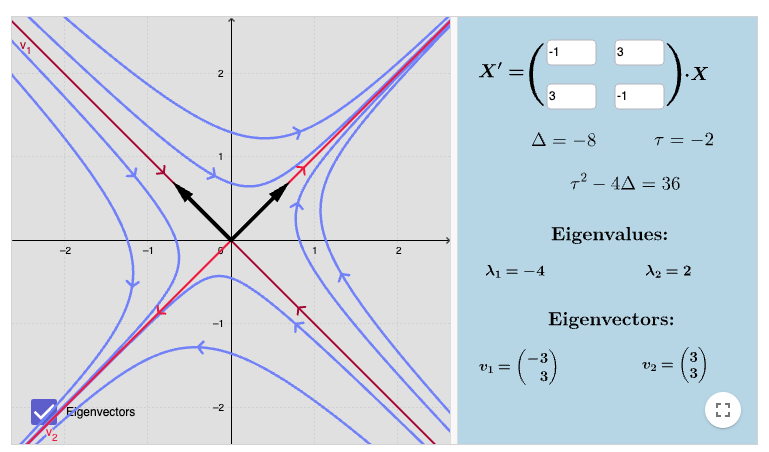
\includegraphics[width=5in]{Images/ImgPhasePlane1331.png}
        \end{center}         
    } 
    \else 
        \begin{center}
        \begin{tikzpicture}[scale=0.85]
        \draw[very thick, ->] (-3, 0) -- (3.25, 0);
        \draw[very thick, ->] (0, -3) -- (0, 3.25);
        \end{tikzpicture}
        \end{center}    
    \fi    

\end{parts}
\fi





\ifnum \Version=7
    \question[6] Consider the IVP $$\vec x \, ' = A\vec x, \quad A = \begin{pmatrix} 0&3\\3&8 \end{pmatrix}, \quad \vec x = \begin{pmatrix} x(t)\\y(t)\end{pmatrix}, \quad \vec x(0) = \begin{pmatrix} -3\\1 \end{pmatrix}$$ The eigenvalues of $A$ are $\lambda_1 = -1$ and $\lambda_2 = 9$. 
    \begin{parts}
        \part Determine the eigenvectors of $A$. Please show your work. 
        
        \ifnum \Solutions=1 {\color{DarkBlue} 
        \textbf{Solutions:}
        For $\lambda_1$:
        \begin{align}
            A - \lambda_1 I = \begin{pmatrix} 1&3\\3&9\end{pmatrix} \ \Rightarrow \ v_1 = \begin{pmatrix} -3\\1 \end{pmatrix}
        \end{align}
        For $\lambda_2$:
        \begin{align}
            A - \lambda_2 I = \begin{pmatrix} -9&3\\3&-1\end{pmatrix} \ \Rightarrow \ v_2 = \begin{pmatrix} 1\\3 \end{pmatrix}
        \end{align}    
        } 
        \else 
            \vspace{6cm}   
        \fi        
        \part Use the given eigenvalues and the eigenvectors that you calculated in part (a) to solve the IVP.  
        
        \ifnum \Solutions=1 {\color{DarkBlue} 
        \textbf{Solutions:} the general solution to the DE is:
        $$\vec x = c_1 e^{-t}\begin{pmatrix} -3\\1\end{pmatrix} + c_2e^{9t} \begin{pmatrix} 1\\3\end{pmatrix}$$
        Use initial condition:
        \begin{align}
            \begin{pmatrix} -3\\1\end{pmatrix} &= c_1\begin{pmatrix}-3\\1 \end{pmatrix}+ c_2 \begin{pmatrix} 1\\3\end{pmatrix} \ \Rightarrow \ c_1 = 1, c_2 = 0 \ \Rightarrow \ 
            \vec x (t) = e^{-t} \begin{pmatrix} -3\\1\end{pmatrix}
        \end{align}
        } 
        \else 
        \vspace{7cm}
    \fi
    \part Sketch the phase portrait of the system on the axes below. Please indicate the direction of motion on your solution curves and draw the eigenspaces corresponding to real eigenvalues (if any). Please also label your axes. 
    
    \ifnum \Solutions=1 {\color{DarkBlue} 
    \textbf{Solutions:}
        \begin{center}
        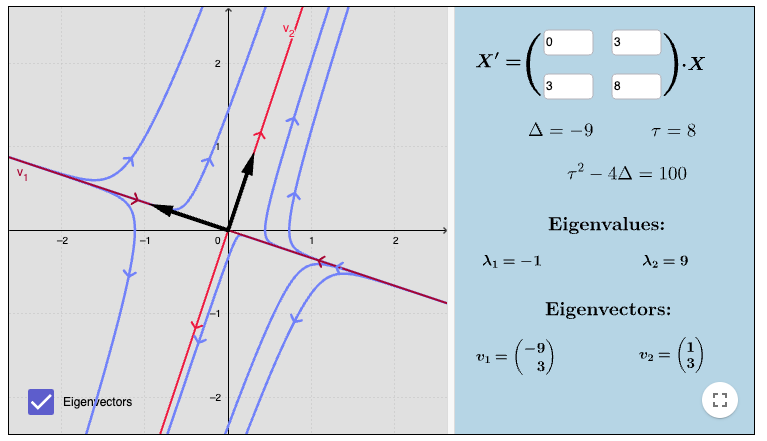
\includegraphics[width=5in]{Images/ImgPhasePlane0338.png}
        \end{center}         
    } 
    \else 
        \begin{center}
        \begin{tikzpicture}[scale=0.85]
        \draw[very thick, ->] (-3, 0) -- (3.25, 0);
        \draw[very thick, ->] (0, -3) -- (0, 3.25);
        \end{tikzpicture}
        \end{center}    
    \fi    

\end{parts}
\fi








\ifnum \Version=8
    \question[6] Consider the IVP $$\vec x \, ' = A\vec x, \quad A = \begin{pmatrix} -1&3\\3&7 \end{pmatrix}, \quad \vec x = \begin{pmatrix} x(t)\\y(t)\end{pmatrix}, \quad \vec x(0) = \begin{pmatrix} 1\\3 \end{pmatrix}$$ The eigenvalues of $A$ are $\lambda_1 = -2$ and $\lambda_2 = 8$. 
    \begin{parts}
        \part Determine the eigenvectors of $A$. Please show your work. 
        
        \ifnum \Solutions=1 {\color{DarkBlue} 
        \textbf{Solutions:}
        For $\lambda_1$:
        \begin{align}
            A - \lambda_1 I = \begin{pmatrix} 1&3\\3&9\end{pmatrix} \ \Rightarrow \ v_1 = \begin{pmatrix} -3\\1 \end{pmatrix}
        \end{align}
        For $\lambda_2$:
        \begin{align}
            A - \lambda_2 I = \begin{pmatrix} -9&3\\3&-1\end{pmatrix} \ \Rightarrow \ v_2 = \begin{pmatrix} 1\\3 \end{pmatrix}
        \end{align}    
        } 
        \else 
            \vspace{6cm}   
        \fi        
        \part Use the given eigenvalues and the eigenvectors that you calculated in part (a) to solve the IVP.  
        
        \ifnum \Solutions=1 {\color{DarkBlue} 
        \textbf{Solutions:} the general solution to the DE is:
        $$\vec x = c_1 e^{-4t}\begin{pmatrix} -1\\1\end{pmatrix} + c_2e^{2t} \begin{pmatrix} 1\\1\end{pmatrix}$$
        Use initial condition:
        \begin{align}
            \begin{pmatrix} 1\\3\end{pmatrix} &= c_1\begin{pmatrix}-3\\1 \end{pmatrix}+ c_2 \begin{pmatrix} 1\\3\end{pmatrix} \ \Rightarrow \ c_1 = 0, c_2 = 1 \ \Rightarrow \ 
            \vec x (t) = e^{8t} \begin{pmatrix} 1\\3\end{pmatrix}
        \end{align}
        } 
        \else 
        \vspace{7cm}
    \fi
    \part Sketch the phase portrait of the system on the axes below. Please indicate the direction of motion on your solution curves and draw the eigenspaces corresponding to real eigenvalues (if any). Please also label your axes. 
    
    \ifnum \Solutions=1 {\color{DarkBlue} 
    \textbf{Solutions:}
        \begin{center}
        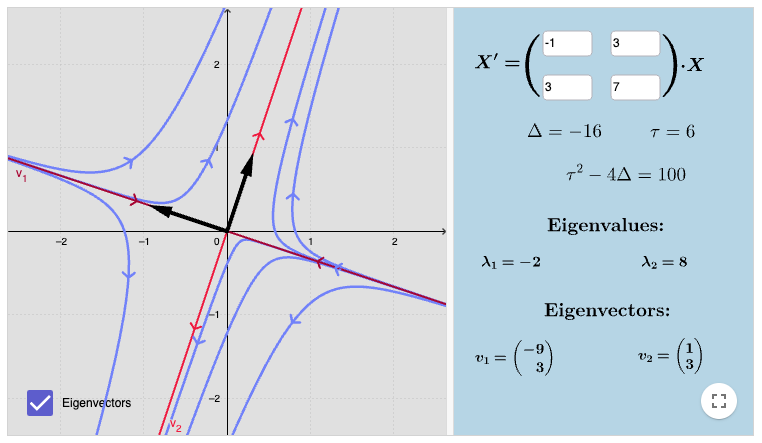
\includegraphics[width=5in]{Images/ImgPhasePlane1337.png}
        \end{center}         
    } 
    \else 
        \begin{center}
        \begin{tikzpicture}[scale=0.85]
        \draw[very thick, ->] (-3, 0) -- (3.25, 0);
        \draw[very thick, ->] (0, -3) -- (0, 3.25);
        \end{tikzpicture}
        \end{center}    
    \fi    

\end{parts}
\fi








\ifnum \Version=9
    \question[6] Consider the IVP $$\vec x \, ' = A\vec x, \quad A = \begin{pmatrix} -2&3\\3&-2 \end{pmatrix}, \quad \vec x = \begin{pmatrix} x(t)\\y(t)\end{pmatrix}, \quad \vec x(0) = \begin{pmatrix} 2\\2 \end{pmatrix}$$ The eigenvalues of $A$ are $\lambda_1 = -5$ and $\lambda_2 = 1$. 
    \begin{parts}
        \part Determine the eigenvectors of $A$. Please show your work. 
        
        \ifnum \Solutions=1 {\color{DarkBlue} 
        \textbf{Solutions:}
        For $\lambda_1$:
        \begin{align}
            A - \lambda_1 I = \begin{pmatrix} 3&3\\3&3\end{pmatrix} \ \Rightarrow \ v_1 = \begin{pmatrix} -1\\1 \end{pmatrix}
        \end{align}
        For $\lambda_2$:
        \begin{align}
            A - \lambda_2 I = \begin{pmatrix} -3&3\\3&-3\end{pmatrix} \ \Rightarrow \ v_2 = \begin{pmatrix} 1\\1 \end{pmatrix}
        \end{align}    
        } 
        \else 
            \vspace{6cm}   
        \fi        
        \part Use the given eigenvalues and the eigenvectors that you calculated in part (a) to solve the IVP.  
        
        \ifnum \Solutions=1 {\color{DarkBlue} 
        \textbf{Solutions:} the general solution to the DE is:
        $$\vec x = c_1 e^{-5t}\begin{pmatrix} -1\\1\end{pmatrix} + c_2e^{t} \begin{pmatrix} 1\\1\end{pmatrix}$$
        Use initial condition:
        \begin{align}
            \begin{pmatrix} 2\\2\end{pmatrix} &= c_1\begin{pmatrix}-1\\1 \end{pmatrix}+ c_2 \begin{pmatrix} 1\\1\end{pmatrix} \ \Rightarrow \ c_1 = 0, c_2 = 2 \ \Rightarrow \ 
            \vec x (t) = 2e^{t} \begin{pmatrix} 1\\1\end{pmatrix}
        \end{align}
        } 
        \else 
        \vspace{7cm}
    \fi
    \part Sketch the phase portrait of the system on the axes below. Please indicate the direction of motion on your solution curves and draw the eigenspaces corresponding to real eigenvalues (if any). Please also label your axes. 
    
    \ifnum \Solutions=1 {\color{DarkBlue} 
    \textbf{Solutions:}
        \begin{center}
        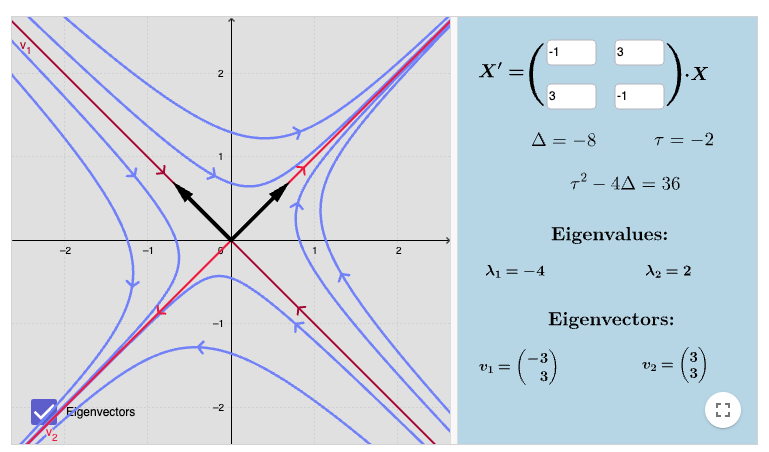
\includegraphics[width=5in]{Images/ImgPhasePlane1331.png}
        \end{center}         
    } 
    \else 
        \begin{center}
        \begin{tikzpicture}[scale=0.85]
        \draw[very thick, ->] (-3, 0) -- (3.25, 0);
        \draw[very thick, ->] (0, -3) -- (0, 3.25);
        \end{tikzpicture}
        \end{center}    
    \fi    

\end{parts}
\fi
    \ifnum \Version=1  
\question[8] Consider the differential equation $\displaystyle \frac{dy}{dt}= (y-2)(y-4k), \ k > 2$. The variable $y$ is a real function of $t$. Assume $y \in  \mathbb R$ and $t \ge 0$.
\fi
\ifnum \Version=2  
\question[8] Consider the differential equation $\displaystyle \frac{dy}{dt}= y^2-9$. The variable $y$ is a real function of $t$. Assume $y \in  \mathbb R$ and $t \ge 0$.
\fi 
\ifnum \Version=3
\question[8] Consider the differential equation $\displaystyle \frac{dy}{dt}= (y-1)(y+2)$. The variable $y$ is a real function of $t$. Assume $y \in  \mathbb R$ and $t \ge 0$.
\fi 
\ifnum \Version=4
\question[8] Consider the differential equation $\displaystyle \frac{dy}{dt}= y^2-4$. The variable $y$ is a real function of $t$. Assume $y \in  \mathbb R$ and $t \ge 0$.
\fi 
\ifnum \Version=5
\question[8] Consider the differential equation $\displaystyle \frac{dy}{dt}= (y+2)(y-3)$. The variable $y$ is a real function of $t$. Assume $y \in  \mathbb R$ and $t \ge 0$.
\fi 

\ifnum \Version<6
\begin{parts}
\part State the critical points of the differential equation.\vspace{1cm}
\part Draw the phase line, and determine whether the critical points (if any) are stable, semi-stable, or unstable.
\vspace{4cm}
\part Determine where $y$ is concave up and where $y$ is concave down for all $y \in \mathbb R$.  Show your work.
\vspace{7cm}
\part Use your results from parts A, B, and C to sketch several solution curves in the $ty$-plane for $y \in \mathbb R$ and $t \ge 0$. Clearly indicate the critical points and the points where the concavity changes. Please label your axes.     
\end{parts}
\fi


\ifnum \Version>5
\question[4] Consider the DE $\displaystyle \dydt = (y-4)(y-8)=y^2-12y+32$. Determine the values of $y$ where the solution curves are concave up and where the curves are concave down. Please show your work. 
\ifnum \Solutions=1 {\color{DarkBlue} 
    \text{Solutions:} Setting $y'=0$ we find that the equilibrium points are $y = 4, 6.$ And if $f(y) = y'$, then $$\dydtt = \dfdy \, \dydt$$ Also 
    $$\dfdy = \ddy\left(y^2-12y+32)\right) = 2y-12 = 2(y-6)$$
    So $df/dy = 0$ when $y=6$. There may be inflection points where either (or both) $df/dy$ and $dy/dt$ are zero. So there could be inflection points at $$y = 4, \ y = 8$$ A table will help determine concavity. When both derivatives have the same sign, the solutions are concave up, and when they have opposite signs the solutions are concave down. 
    \begin{center}            
        \renewcommand{\arraystretch}{1.4}
        \begin{tabular}{c|cccc} 
        $ y $ & $ (-\infty,4) $ & $(4,6)$ & $(6,8)$ & $(8,\infty)$  \\ \hline 
        $\displaystyle  dy/dt=(y-4)(y-8)$ & $+$ & $-$ & $-$ & $+$  \\ \hline
        $ \displaystyle df/dy = 2(y-6) $ & $-$ & $-$ & $+$ & $+$  \\[4pt] \hline
        $ \text{concavity} $ & \text{down} & \text{up} & \text{down} & \text{up} \\ \hline
        \end{tabular}
    \end{center}  
    So concave up on $y>8$ and $4<y<6$. Concave down on $y<4$, and $6<y<8$. 
} 
\else 
\fi
\fi 




        
\end{questions}

% SCRATCH
\ifnum \Solutions=0 \newpage 
    \begin{center}
        \textit{This page can be used for scratch work. }
    \end{center}
\fi
    
\end{document}


